\chapter{Statistical Behaviour}
\label{app:results}
Here we present the graphs the heuristic selection was based on. They
are not commented here.

All level were run for 5 seconds before being killed. Each line
represent a given heuristic/algorithm combination on a level. Note
that these figures say very little about the performance of the
systems, but more about the behaviour of each heuristic.


\begin{figure}
  \centering
  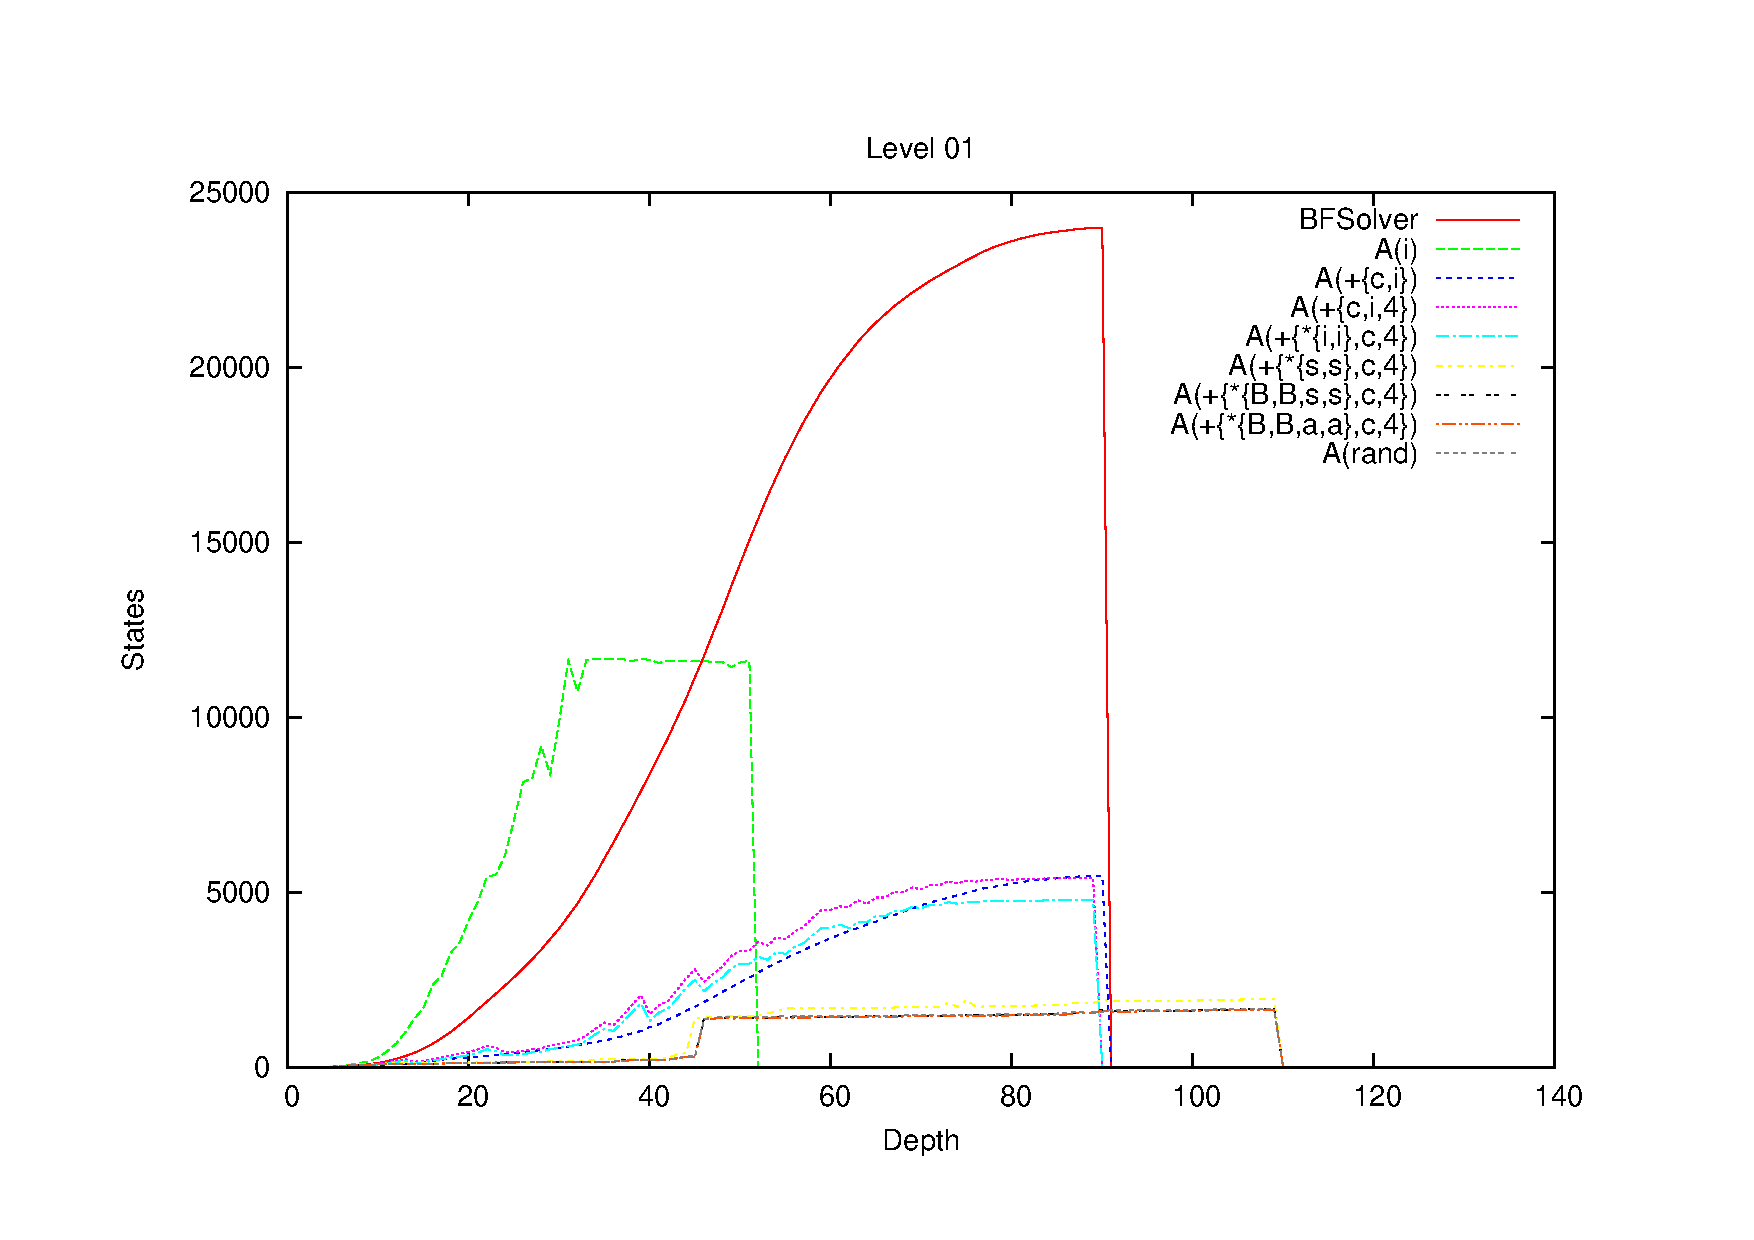
\includegraphics[width=0.85\textwidth]{level01-5}
  \caption{Level 01}
  \label{fig:level01-stats}
\end{figure}
 
\begin{figure}
  \centering
  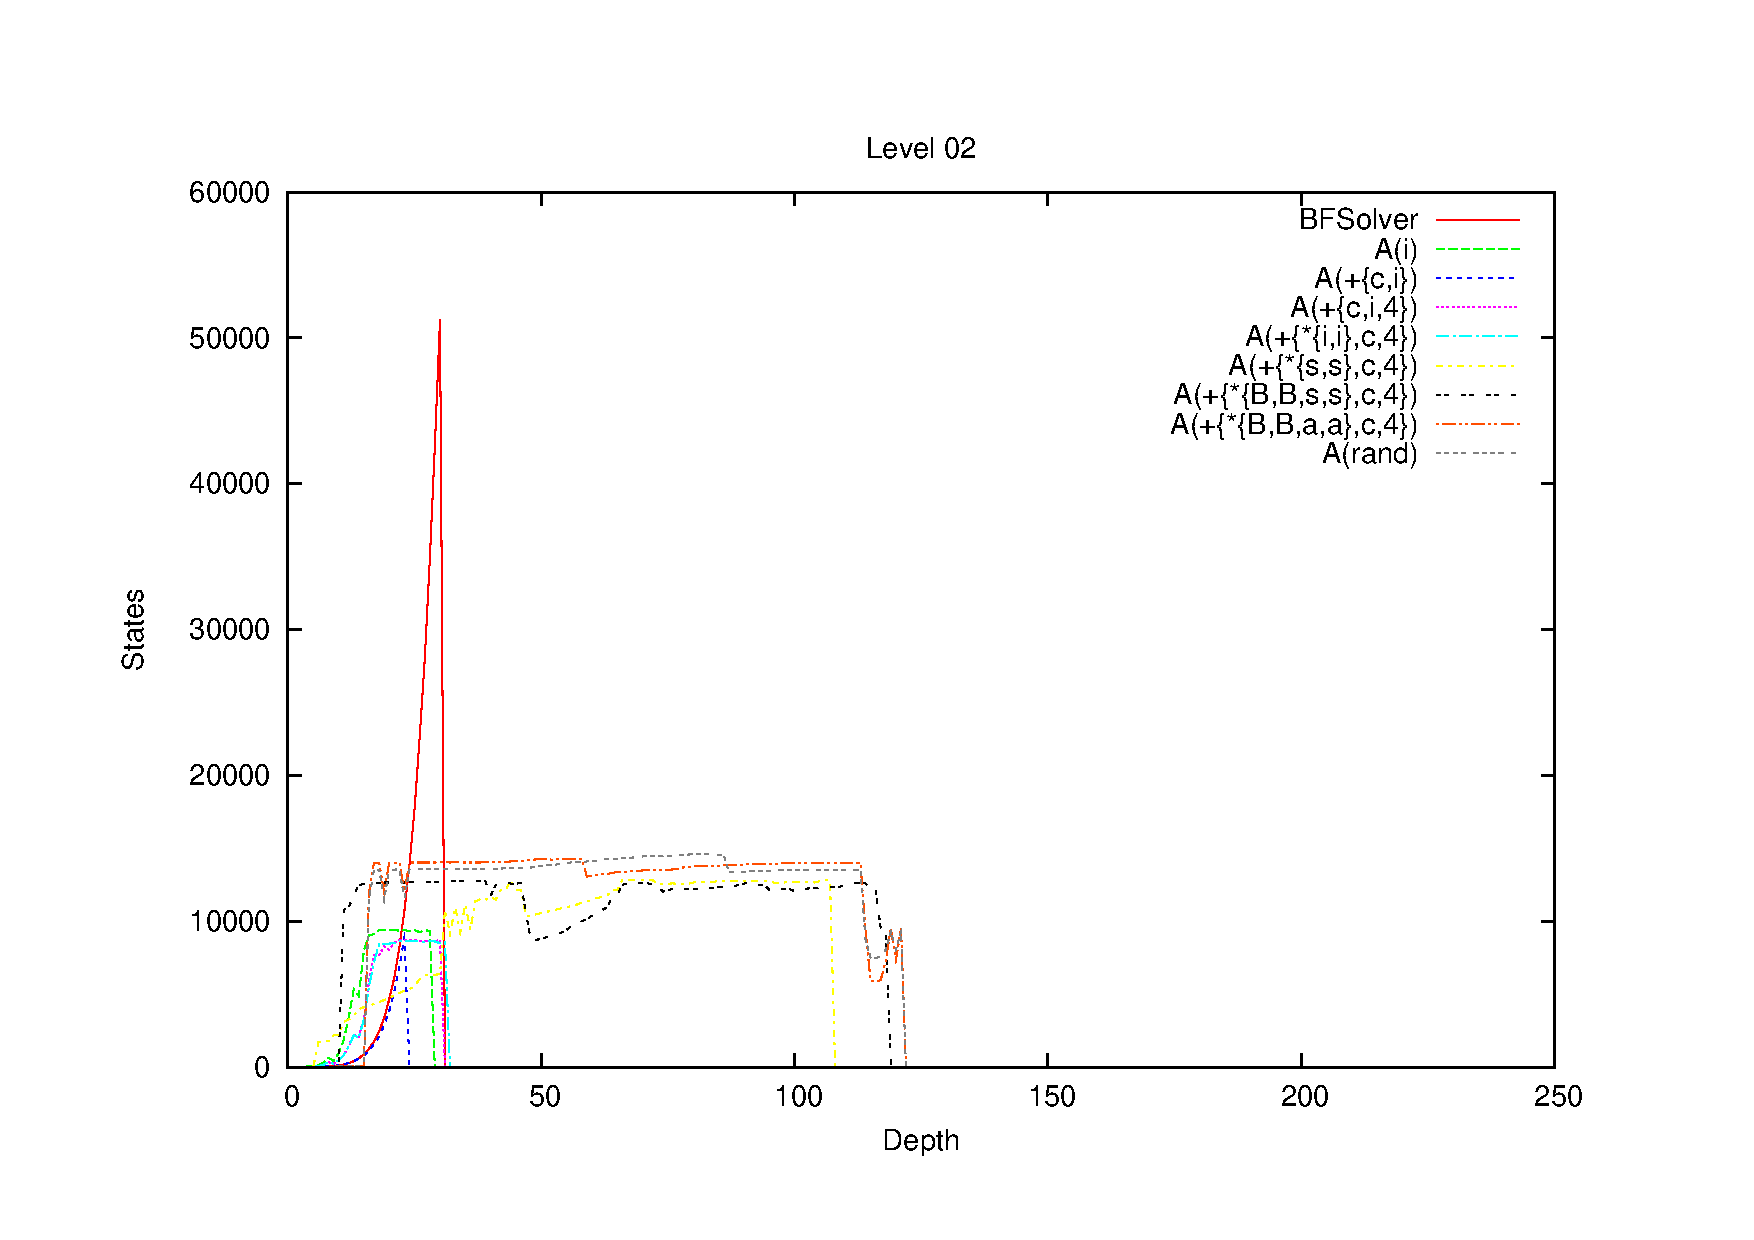
\includegraphics[width=0.85\textwidth]{level02-5}
  \caption{Level 02}
  \label{fig:level02-stats}
\end{figure}

\begin{figure}
  \centering
  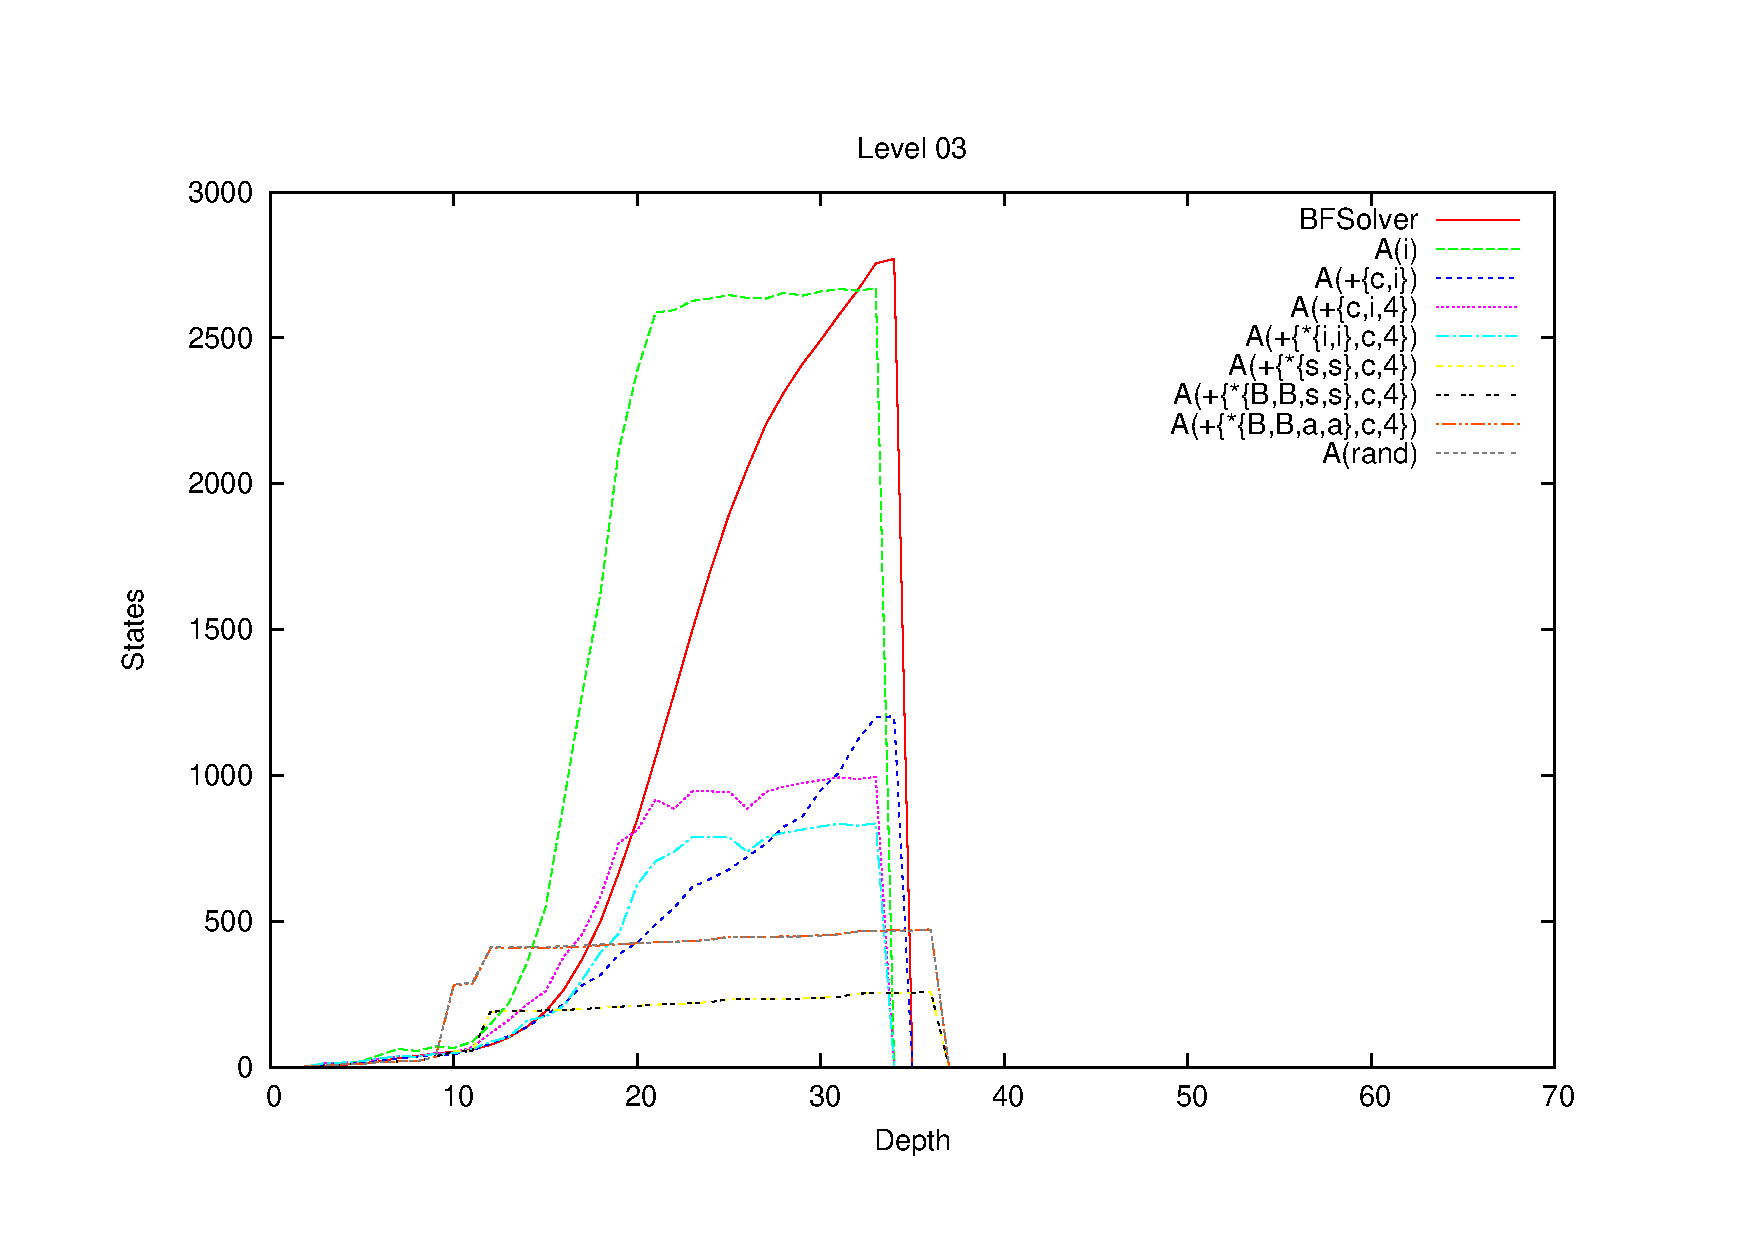
\includegraphics[width=0.85\textwidth]{level03-5}
  \caption{Level 03}
  \label{fig:level03-stats}
\end{figure}
 
\begin{figure}
  \centering
  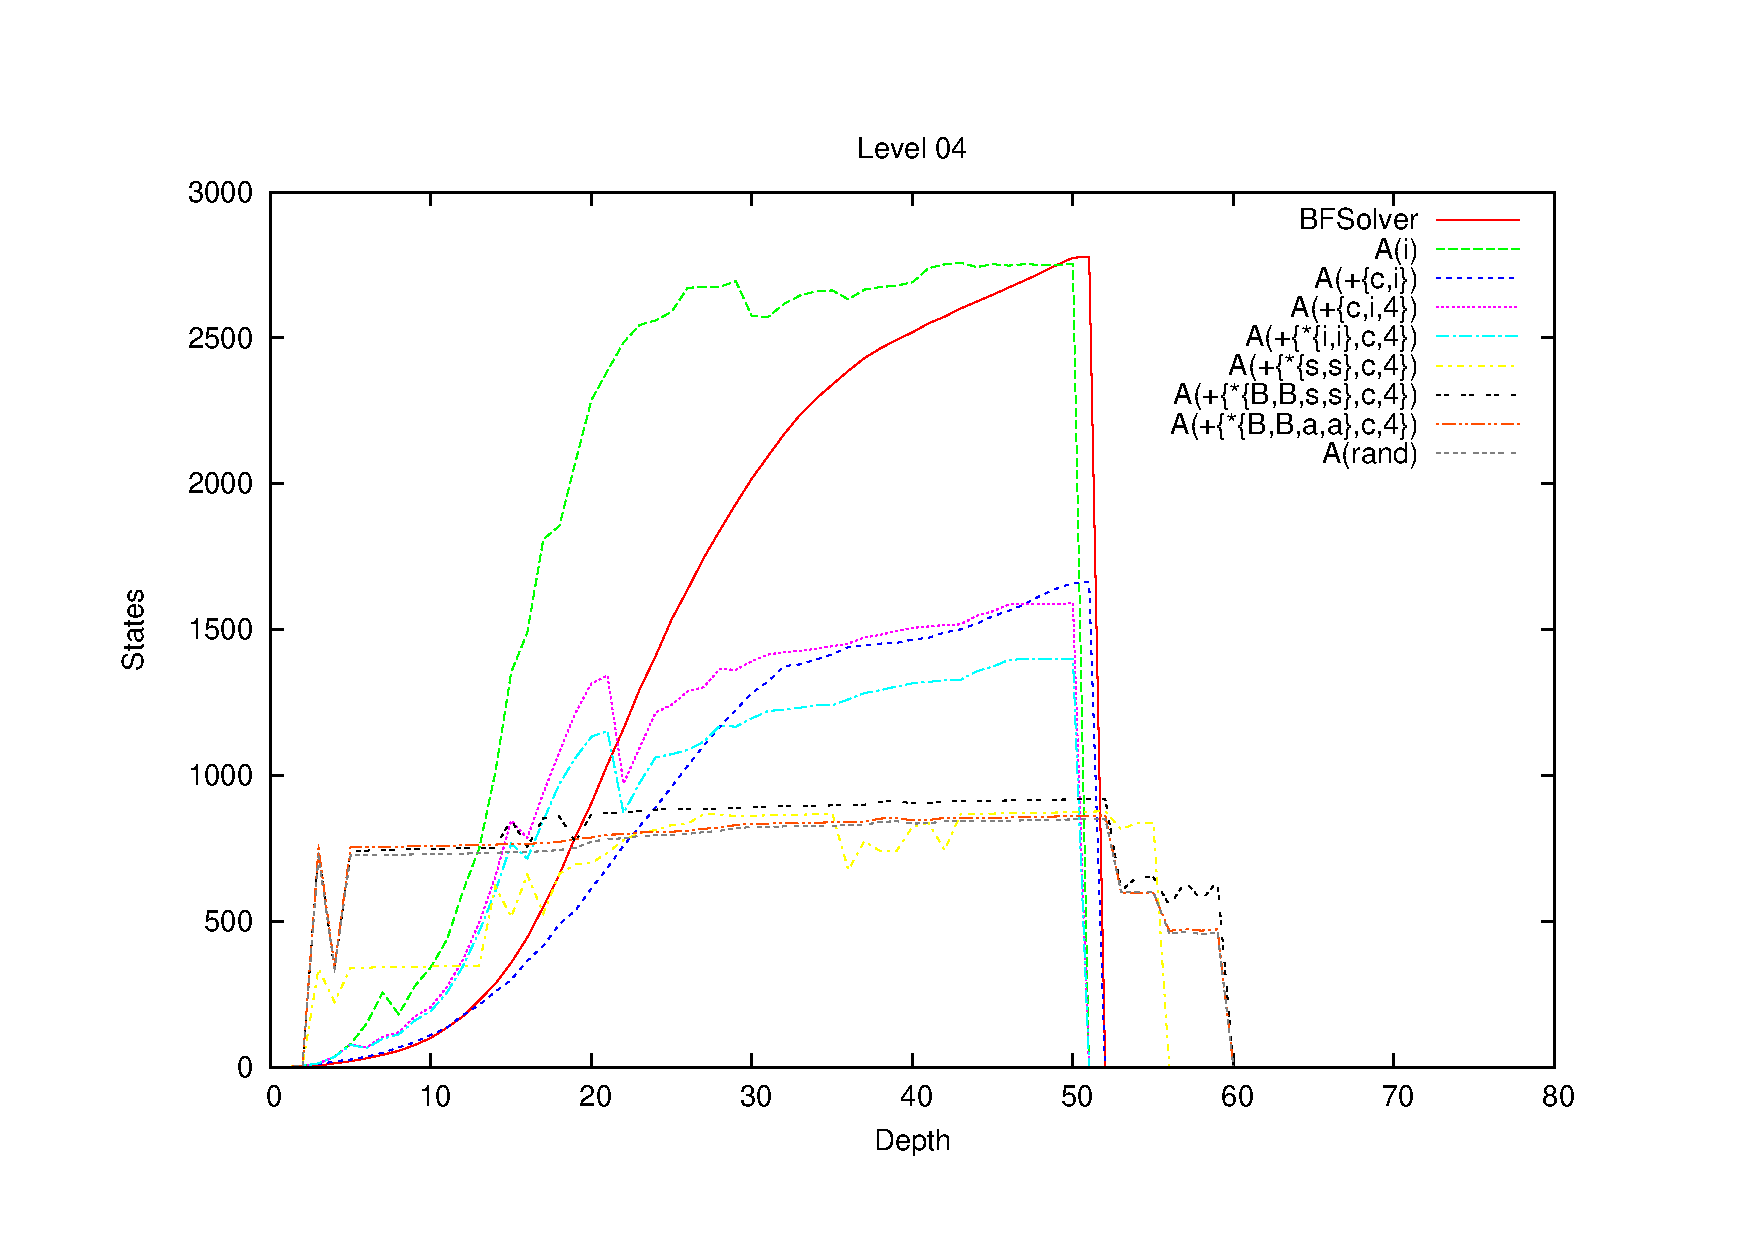
\includegraphics[width=0.85\textwidth]{level04-5}
  \caption{Level 04}
  \label{fig:level04-stats}
\end{figure}

\begin{figure}
  \centering
  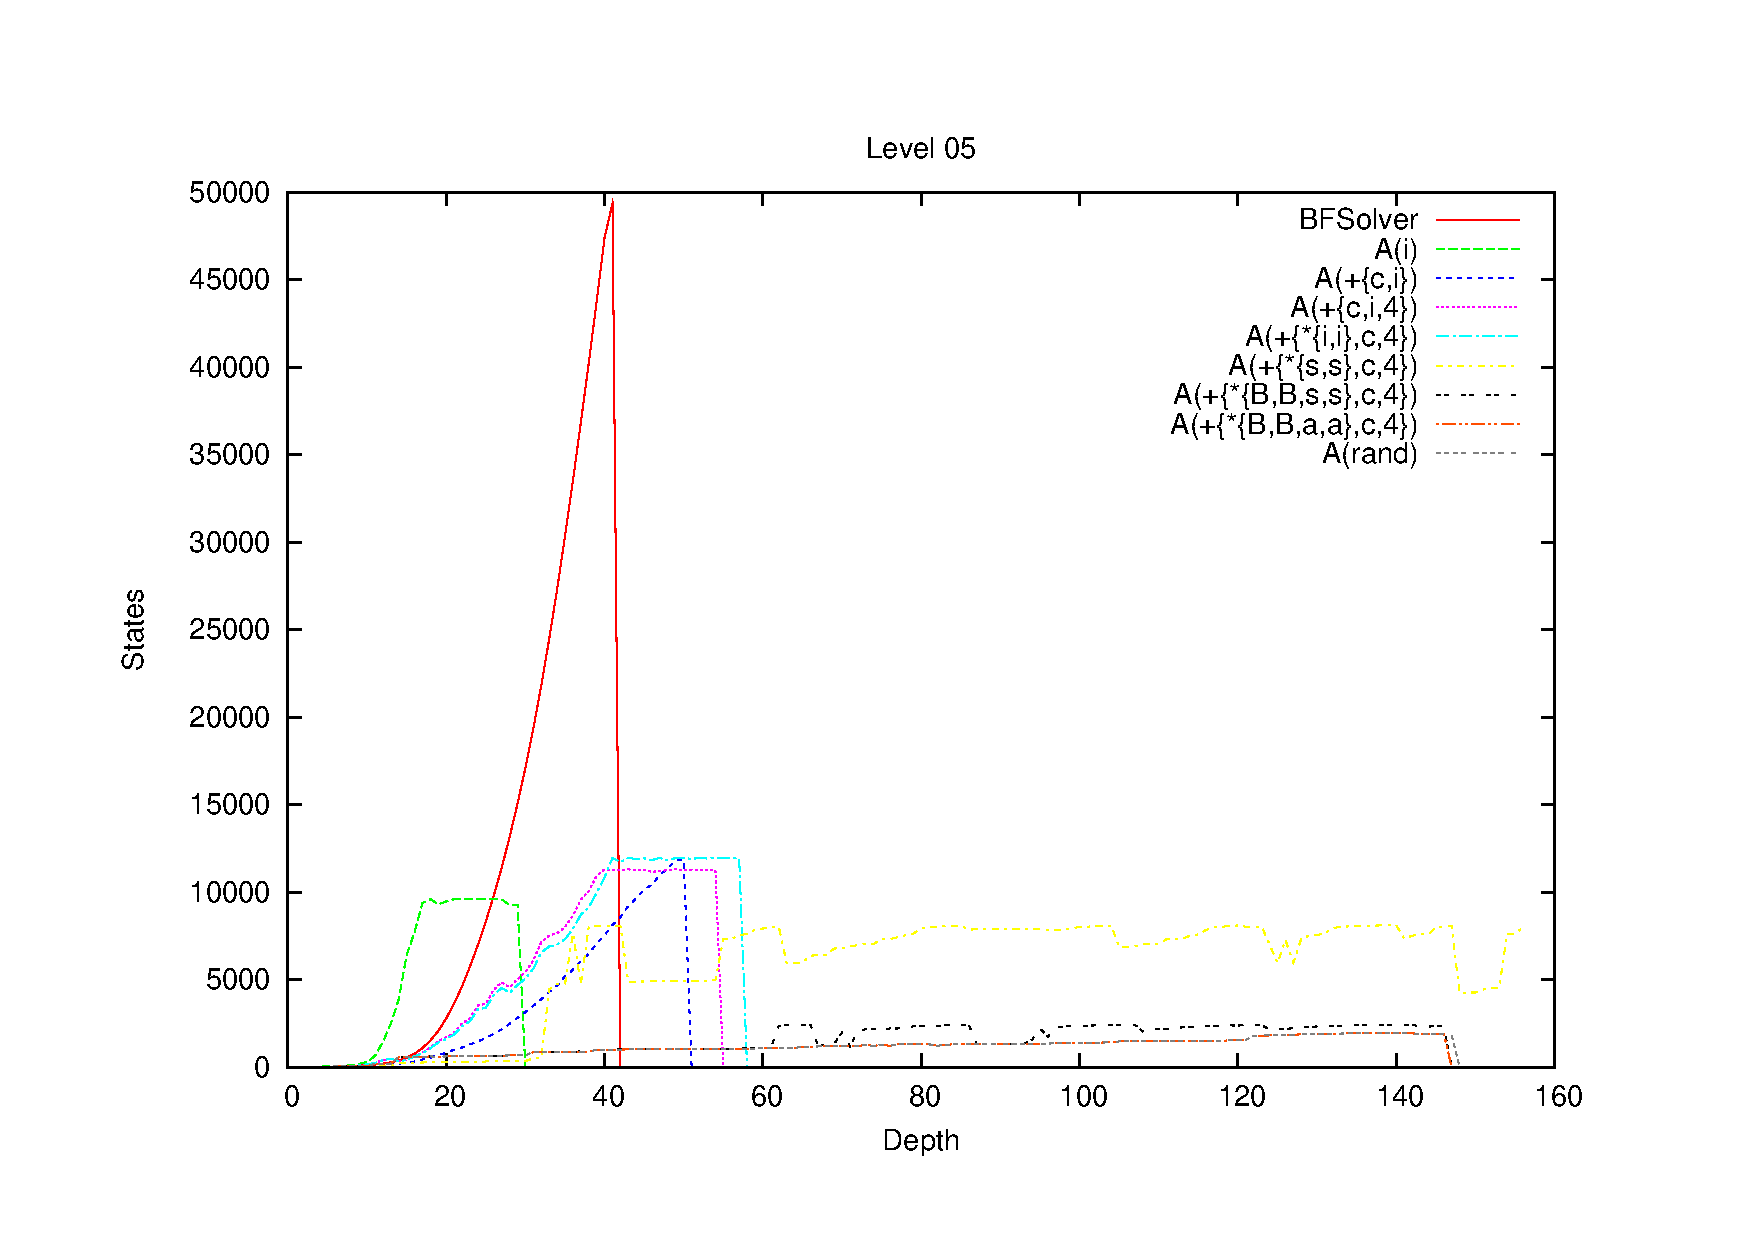
\includegraphics[width=0.85\textwidth]{level05-5}
  \caption{Level 05}
  \label{fig:level05-stats}
\end{figure}
 
\begin{figure}
  \centering
  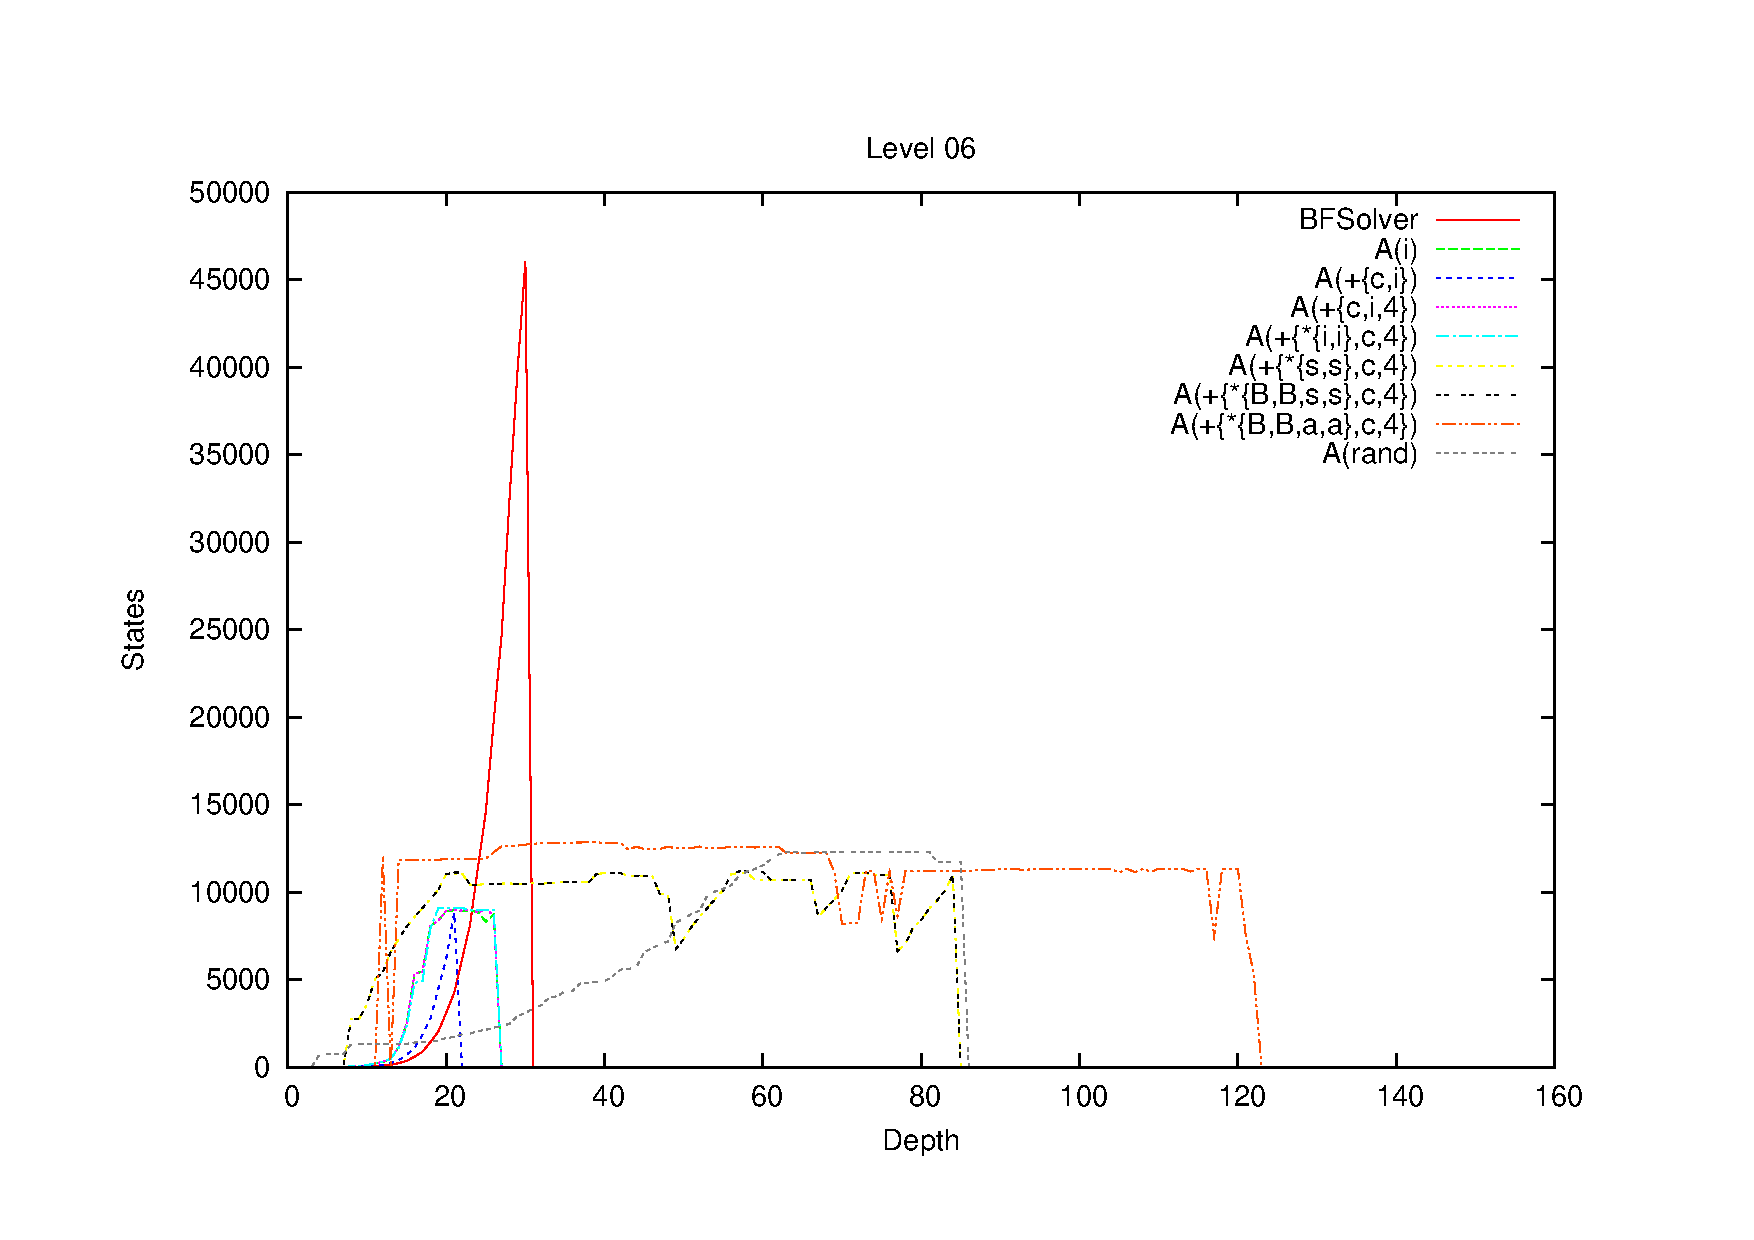
\includegraphics[width=0.85\textwidth]{level06-5}
  \caption{Level 06}
  \label{fig:level06-stats}
\end{figure}

\begin{figure}
  \centering
  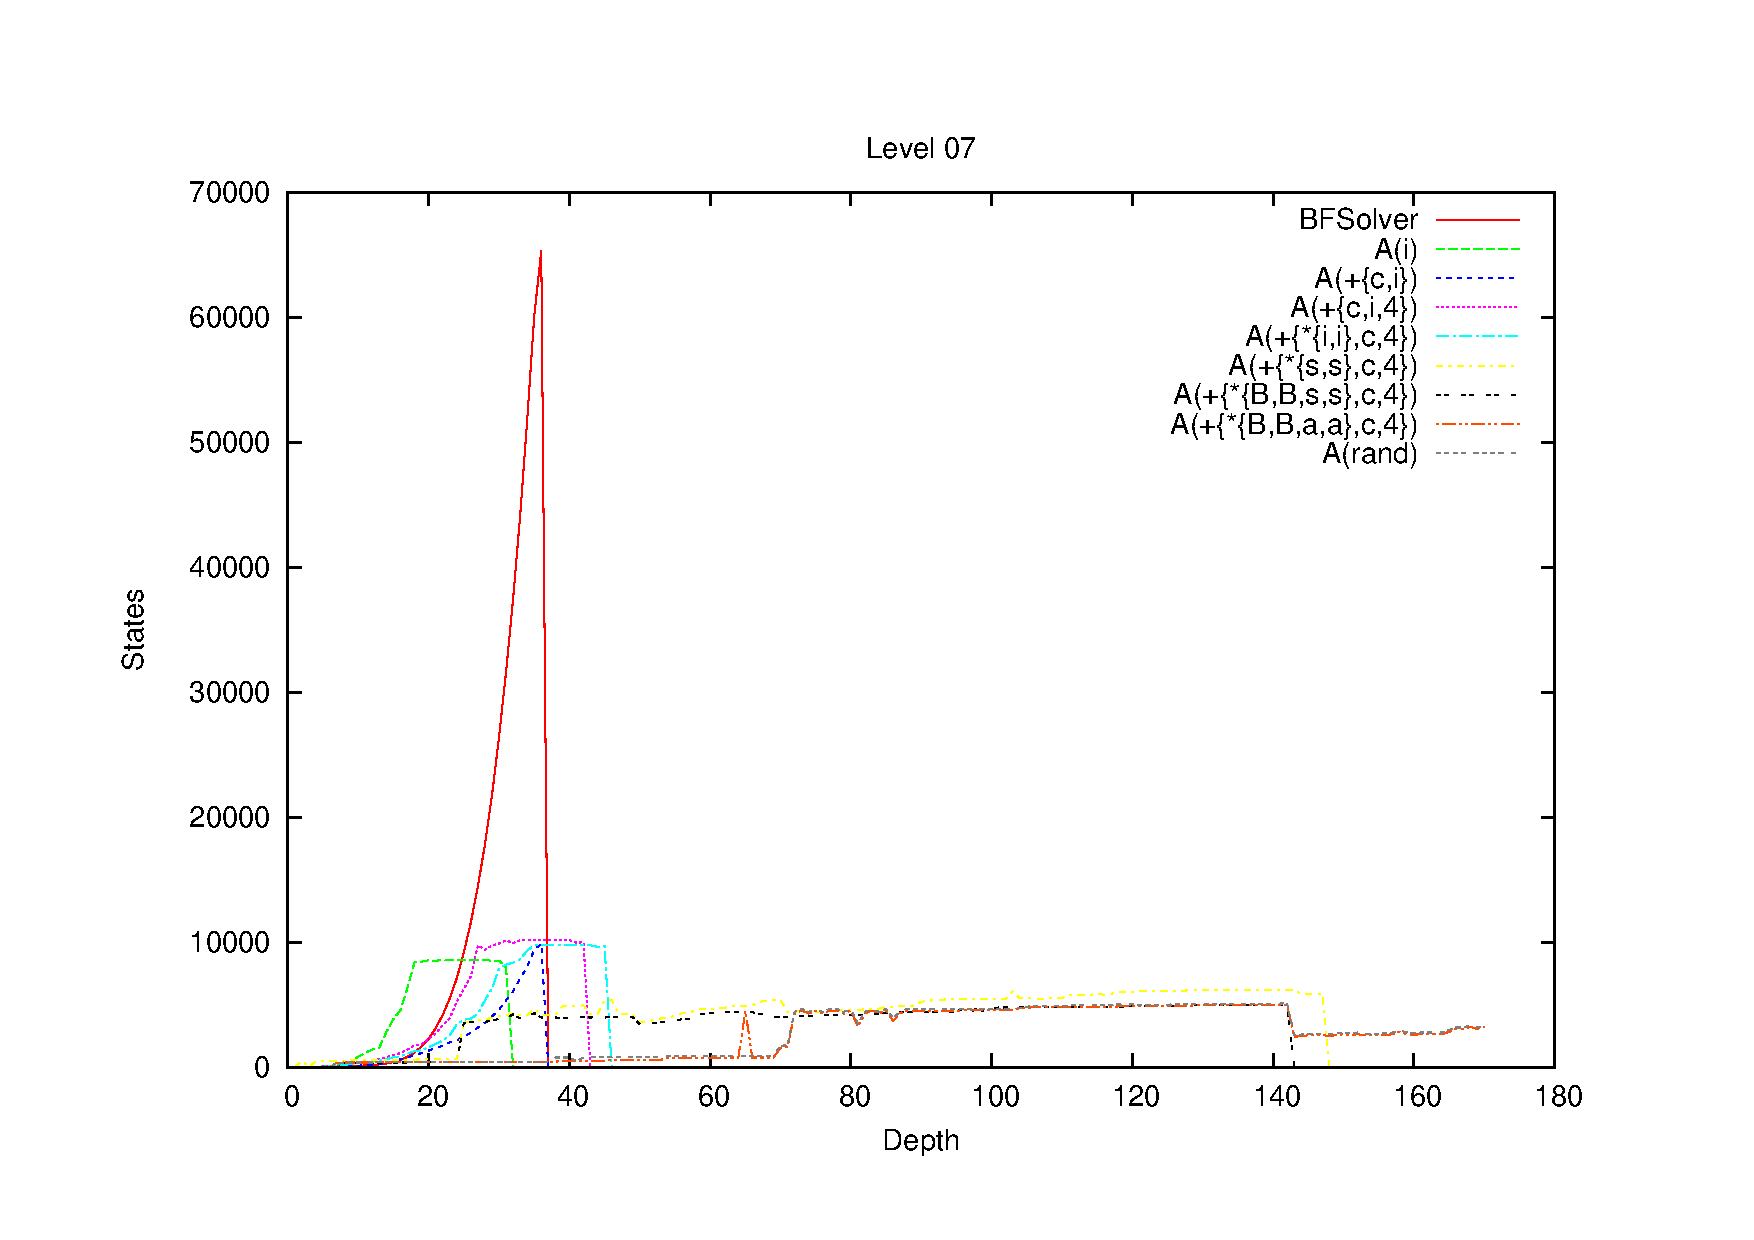
\includegraphics[width=0.85\textwidth]{level07-5}
  \caption{Level 07}
  \label{fig:level07-stats}
\end{figure}
 
\begin{figure}
  \centering
  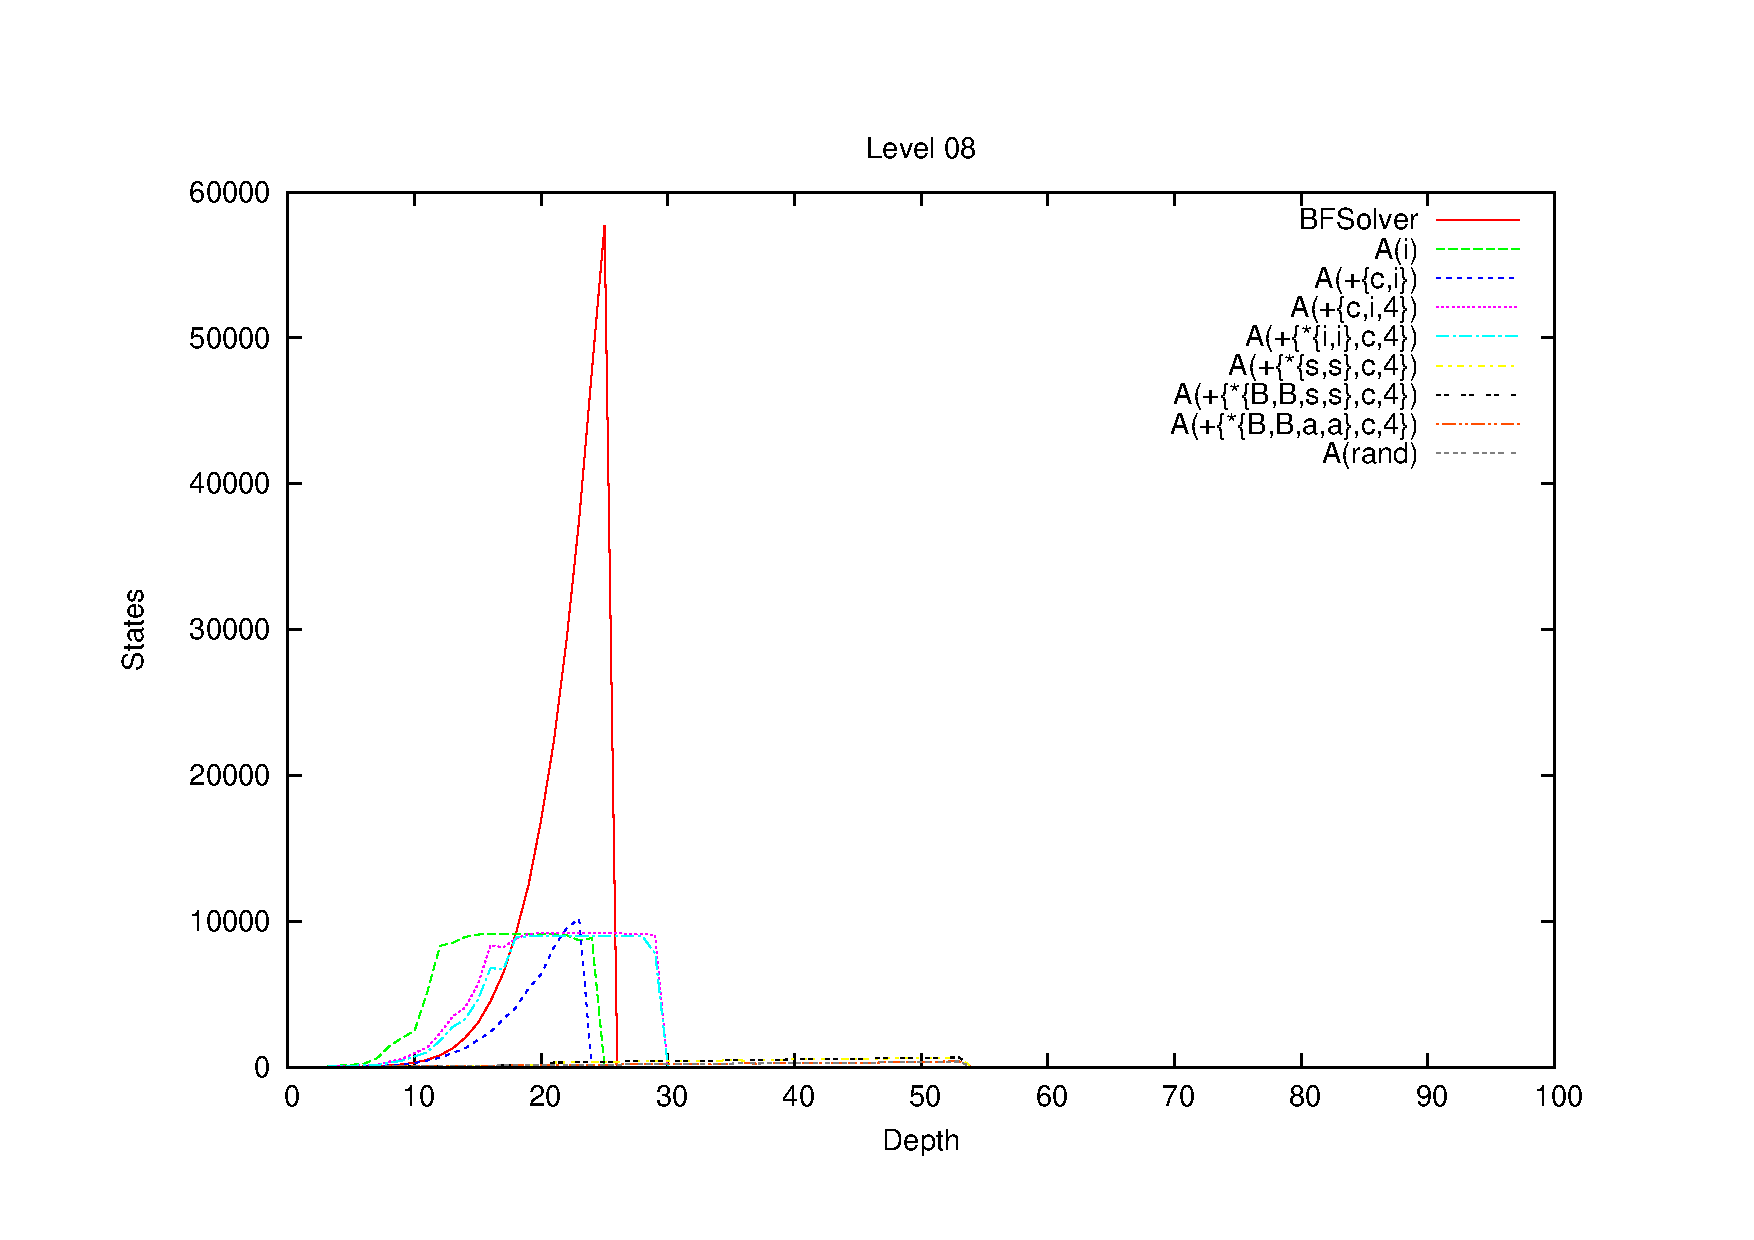
\includegraphics[width=0.85\textwidth]{level08-5}
  \caption{Level 08}
  \label{fig:level08-stats}
\end{figure}

\begin{figure}
  \centering
  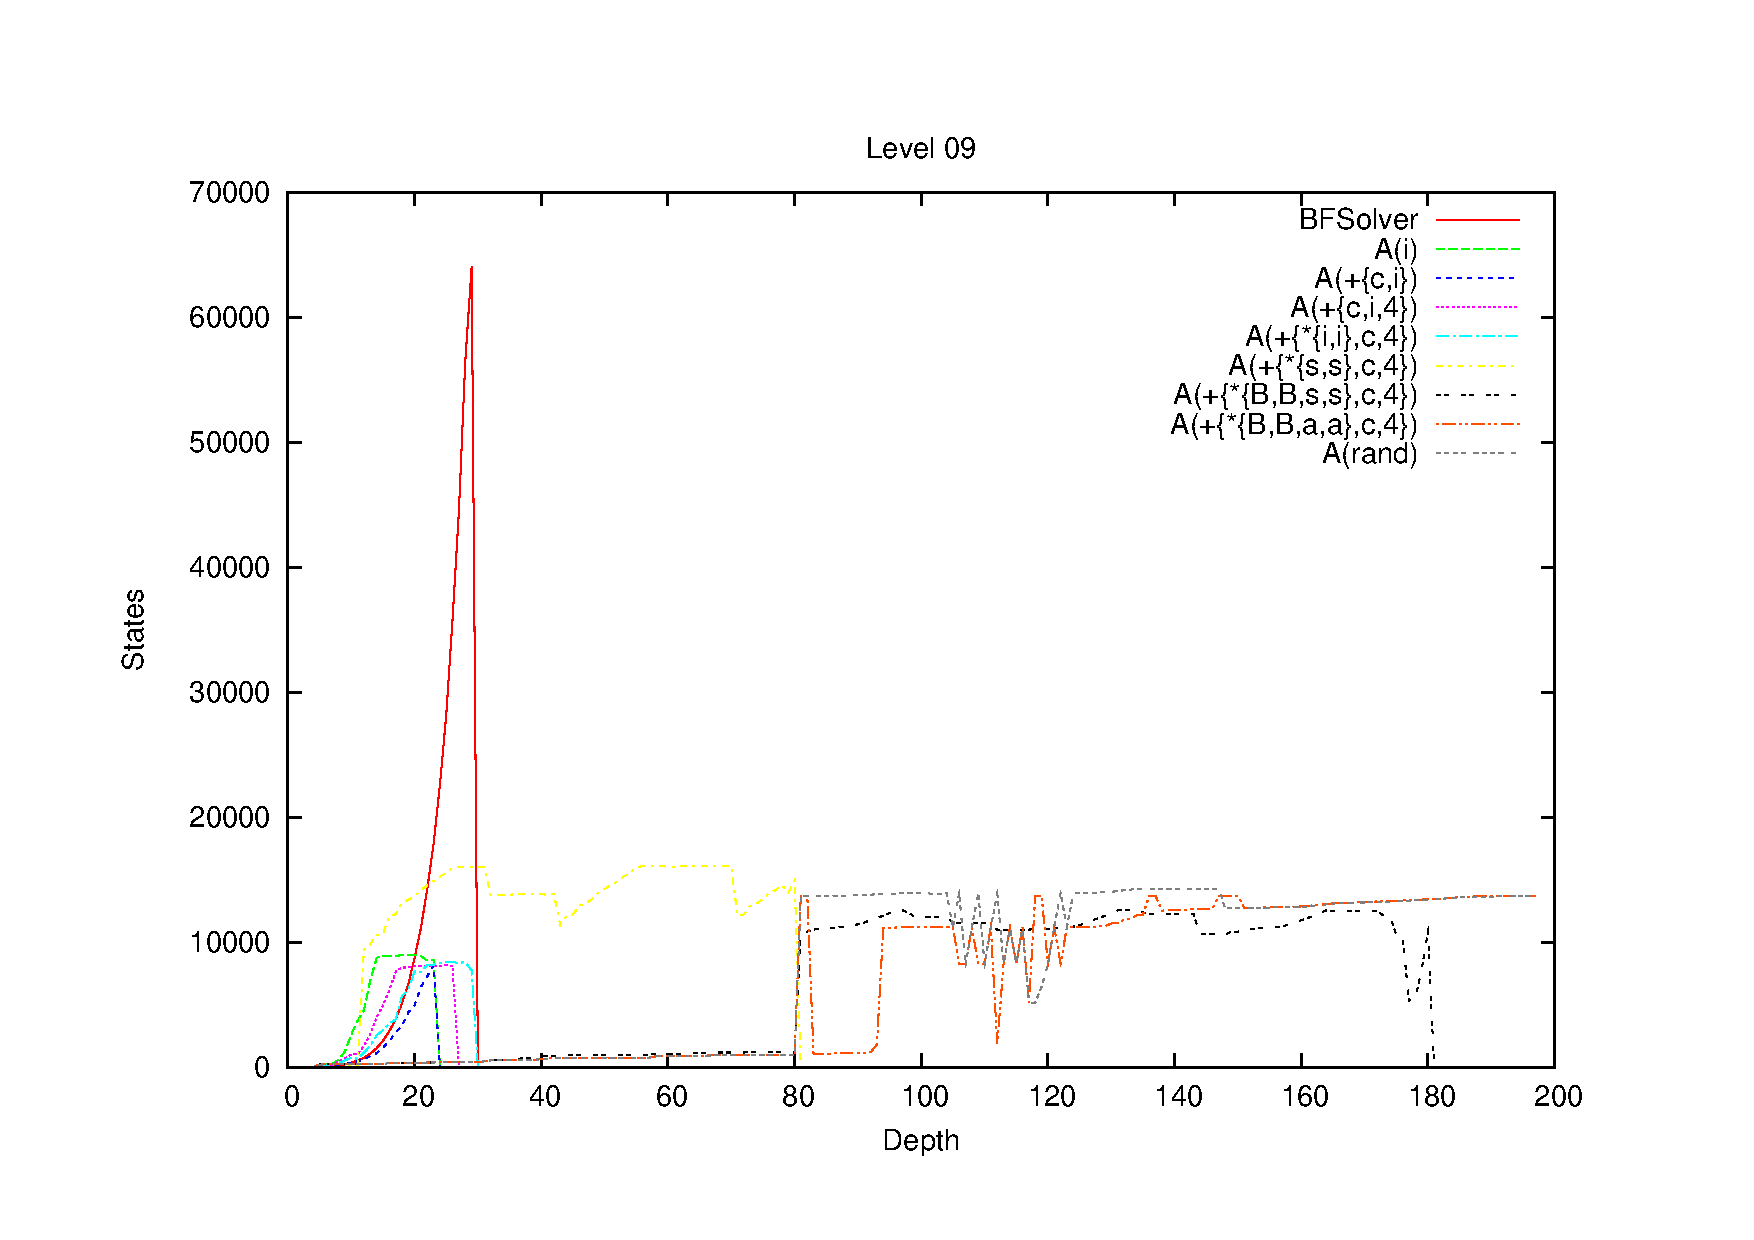
\includegraphics[width=0.85\textwidth]{level09-5}
  \caption{Level 09}
  \label{fig:level09-stats}
\end{figure}
 
\begin{figure}
  \centering
  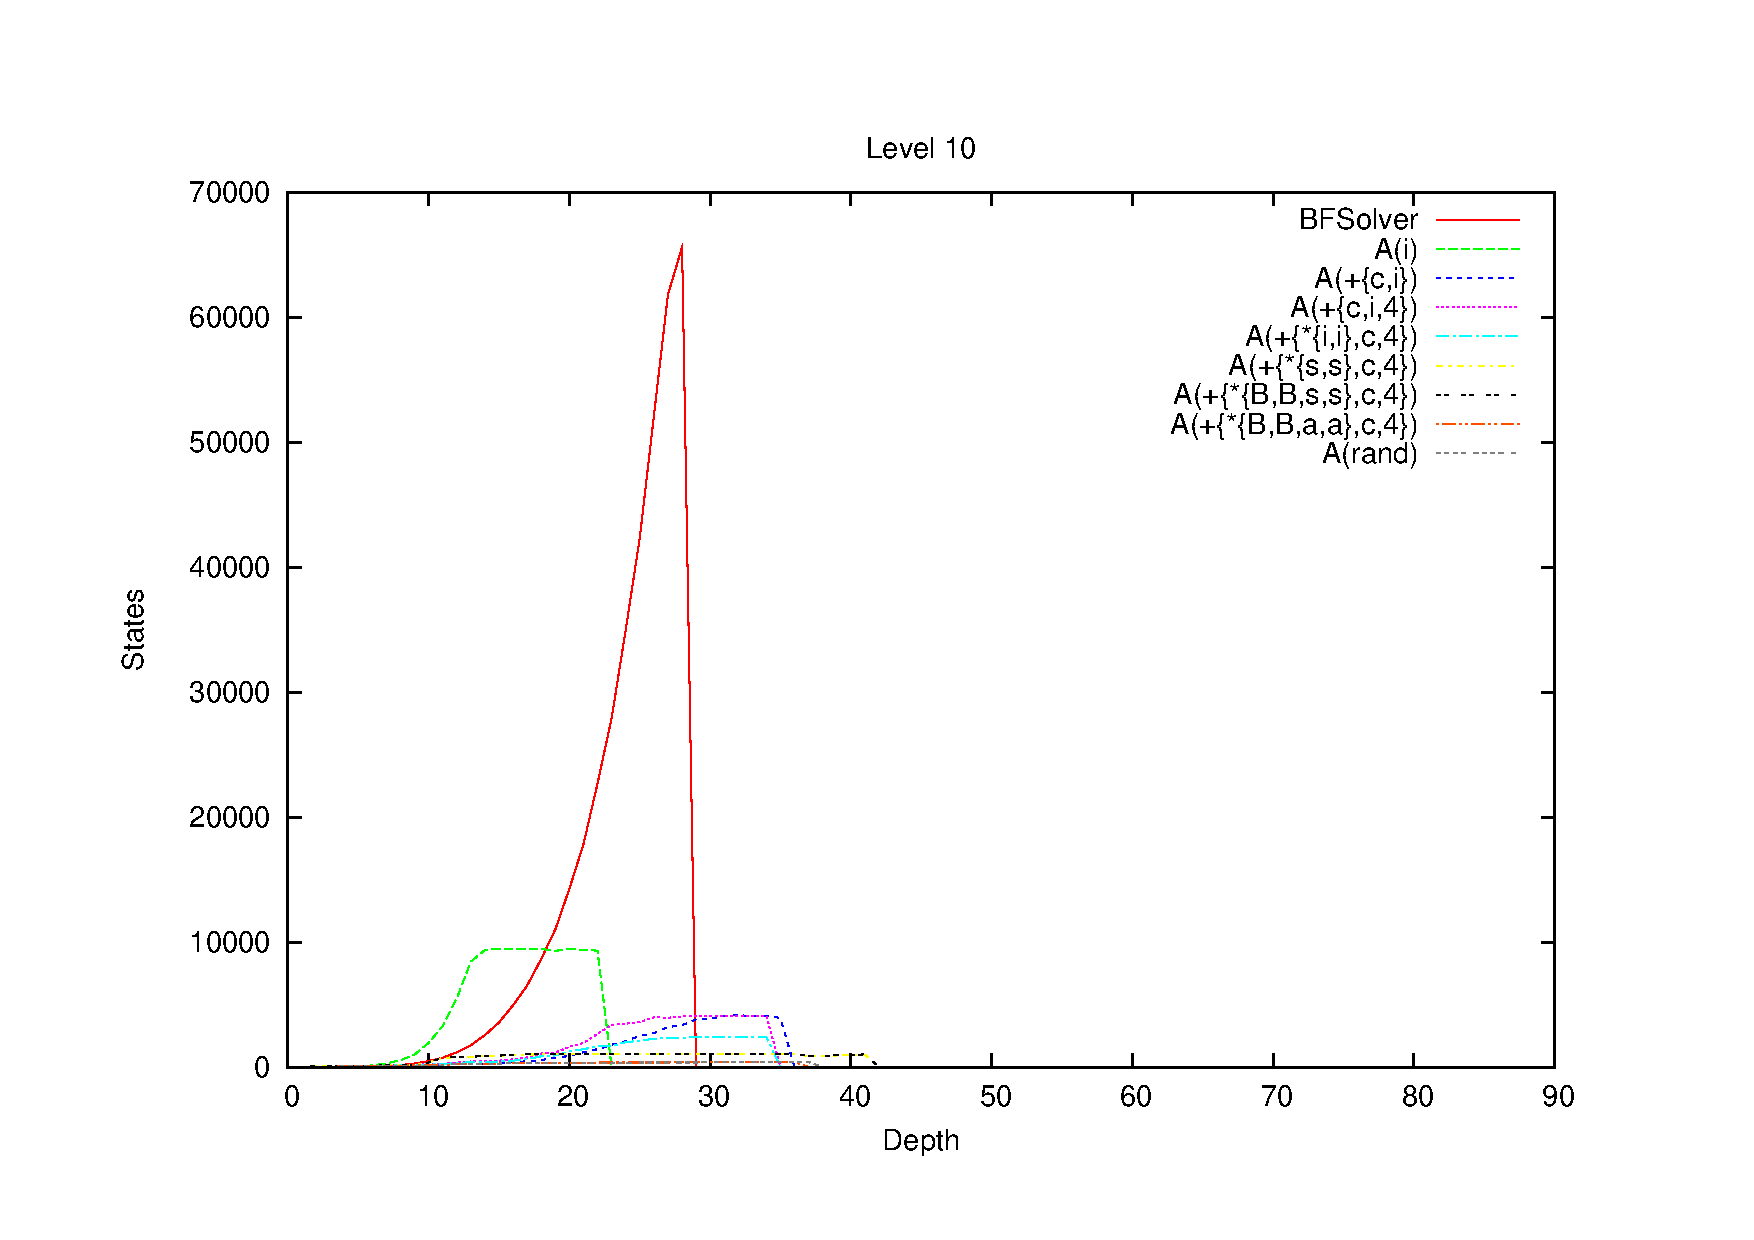
\includegraphics[width=0.85\textwidth]{level10-5}
  \caption{Level 10}
  \label{fig:level10-stats}
\end{figure}

\clearpage

\begin{figure}
  \centering
  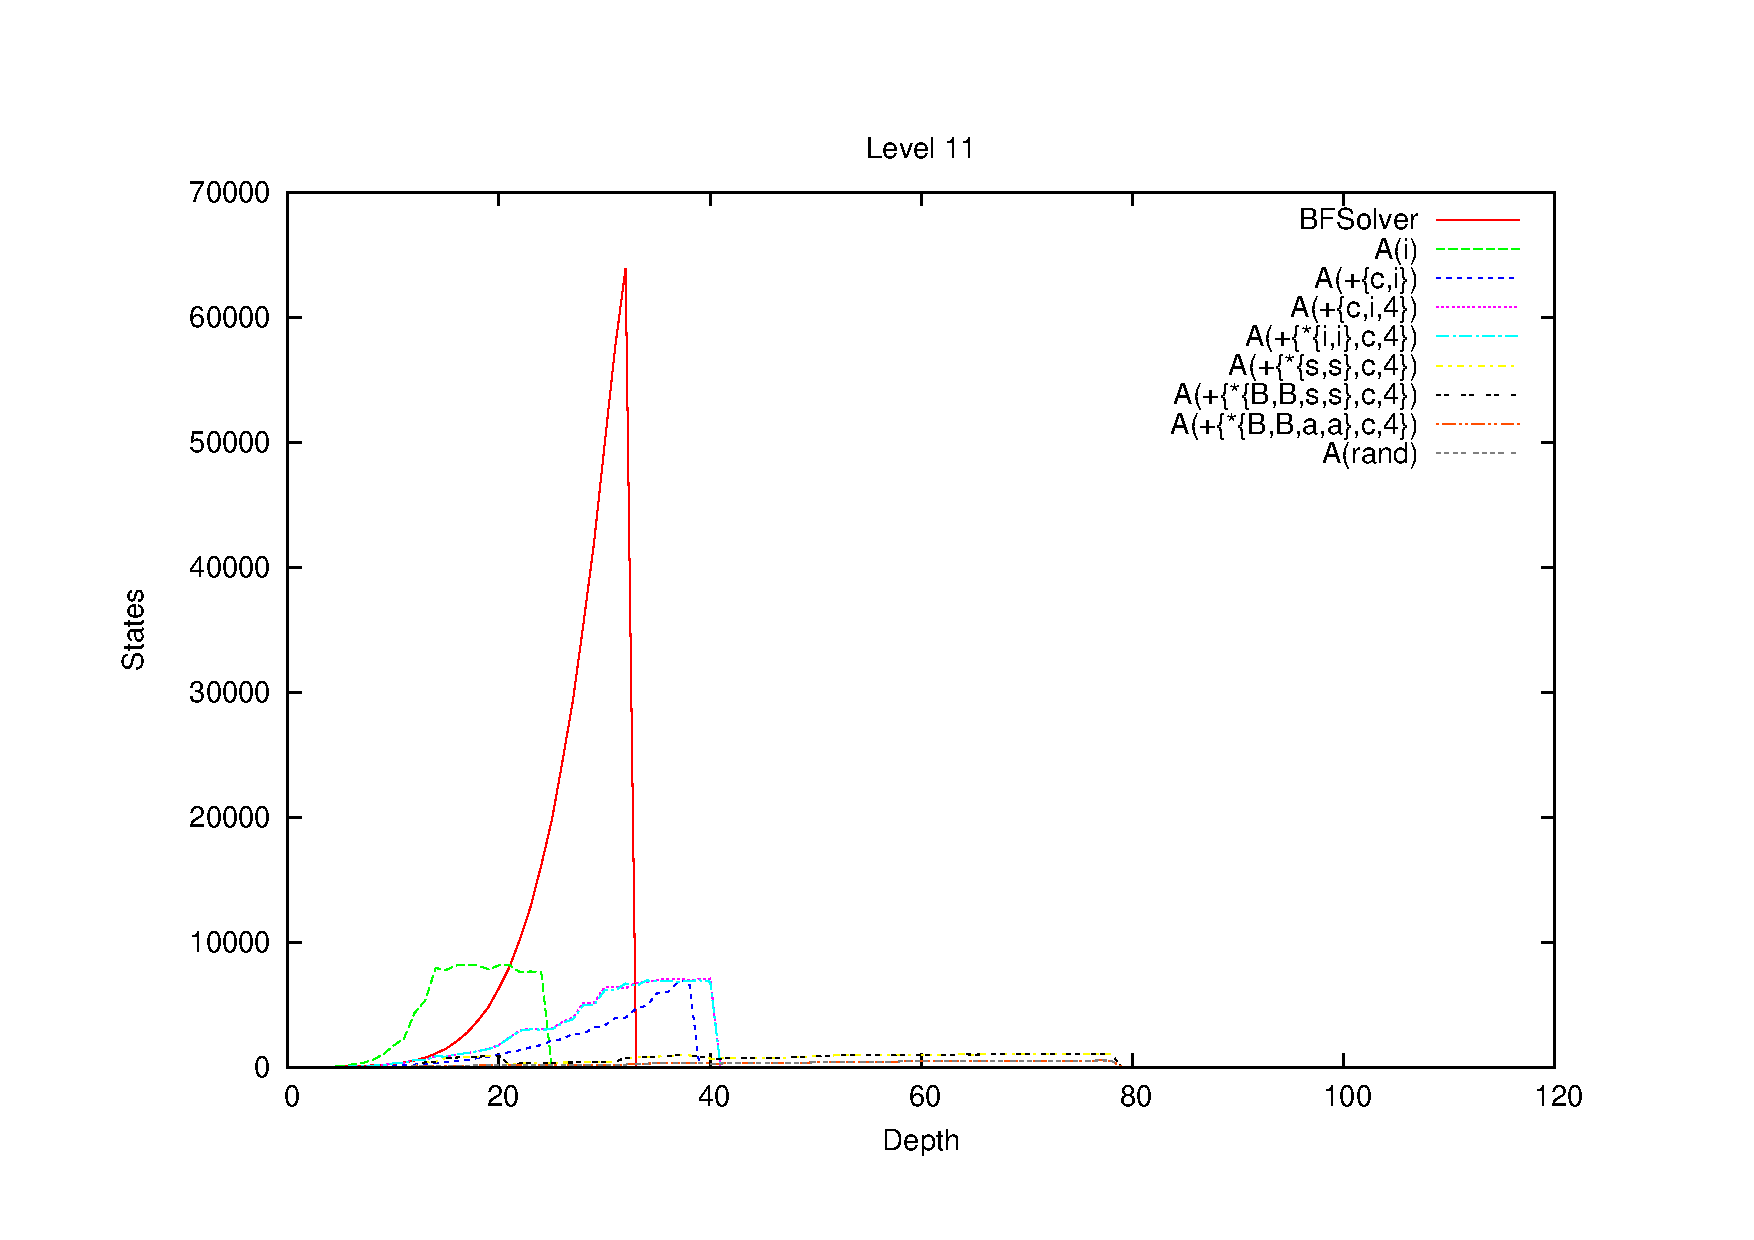
\includegraphics[width=0.85\textwidth]{level11-5}
  \caption{Level 11}
  \label{fig:level11-stats}
\end{figure}
 
\begin{figure}
  \centering
  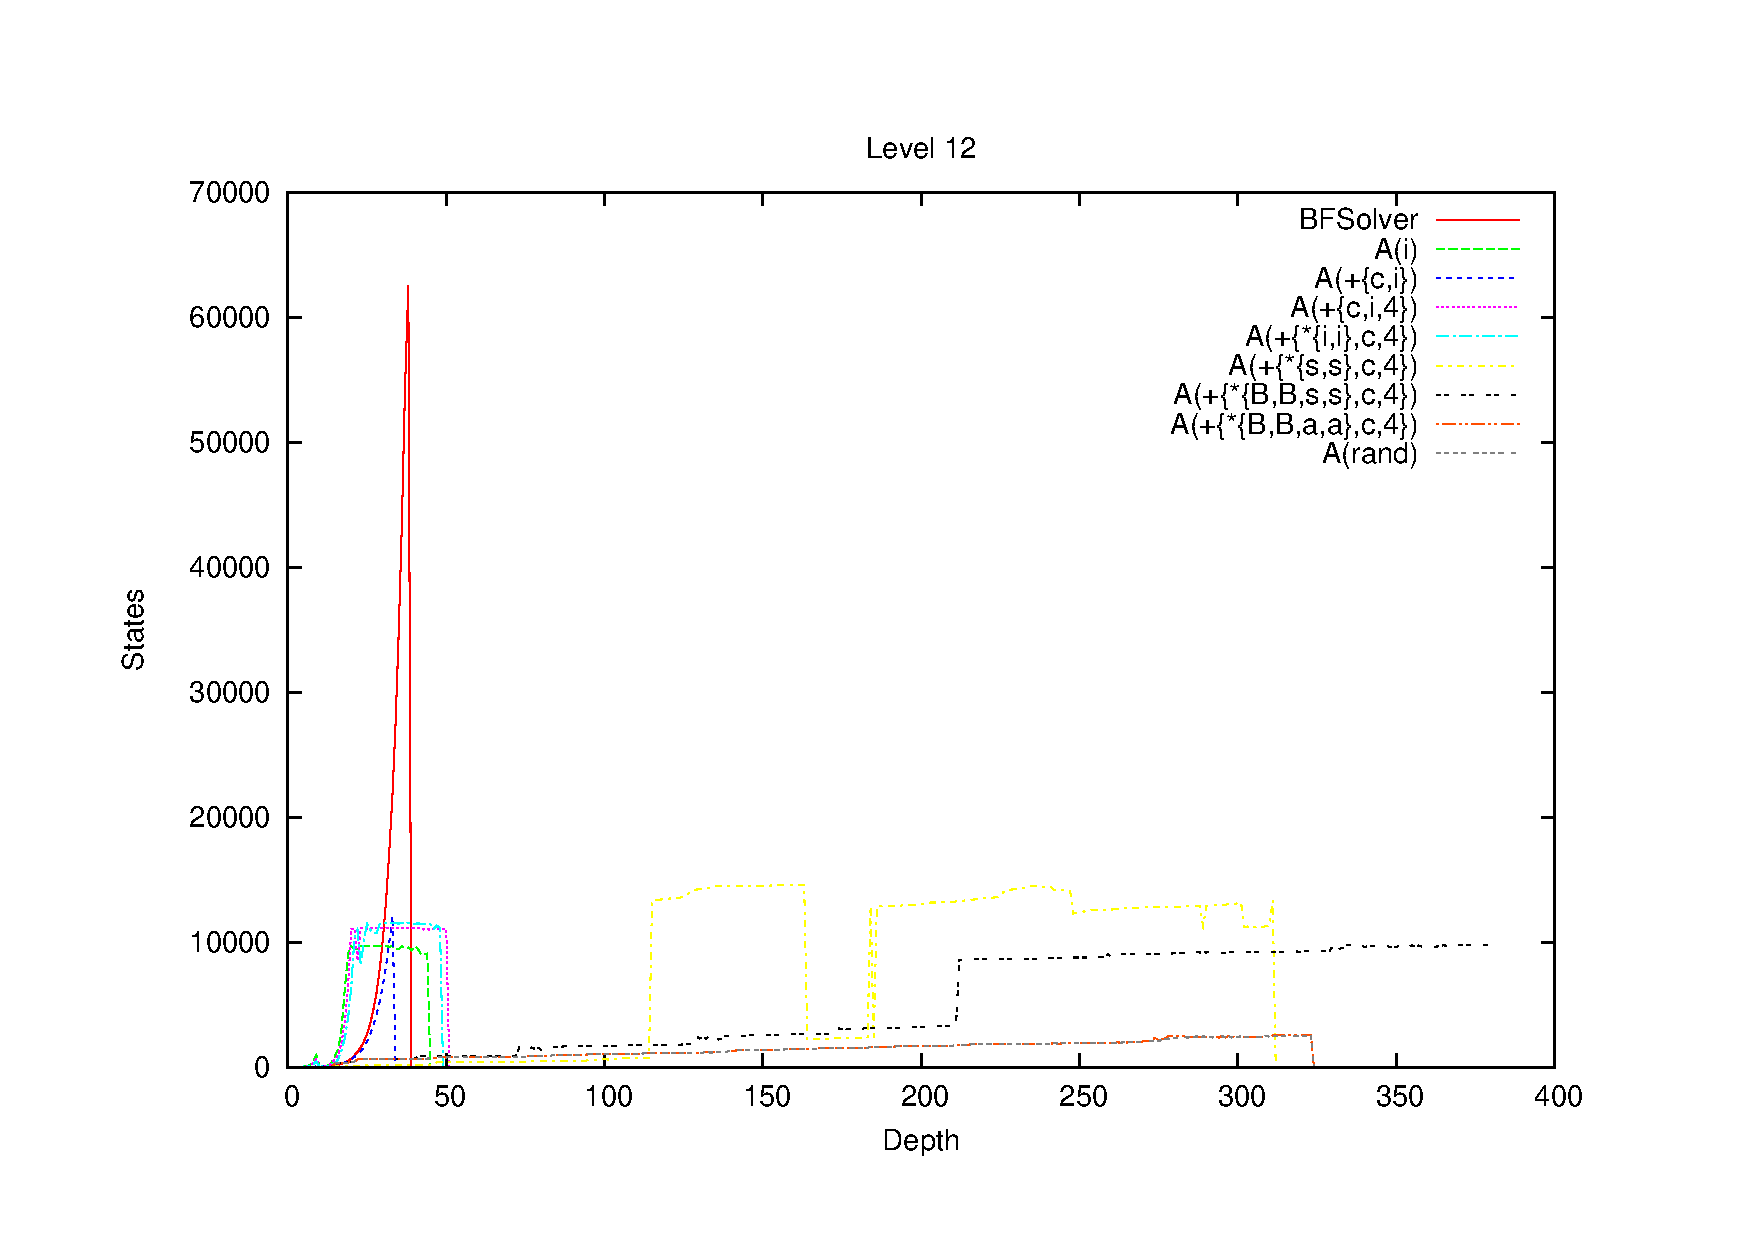
\includegraphics[width=0.85\textwidth]{level12-5}
  \caption{Level 12}
  \label{fig:level12-stats}
\end{figure}

\begin{figure}
  \centering
  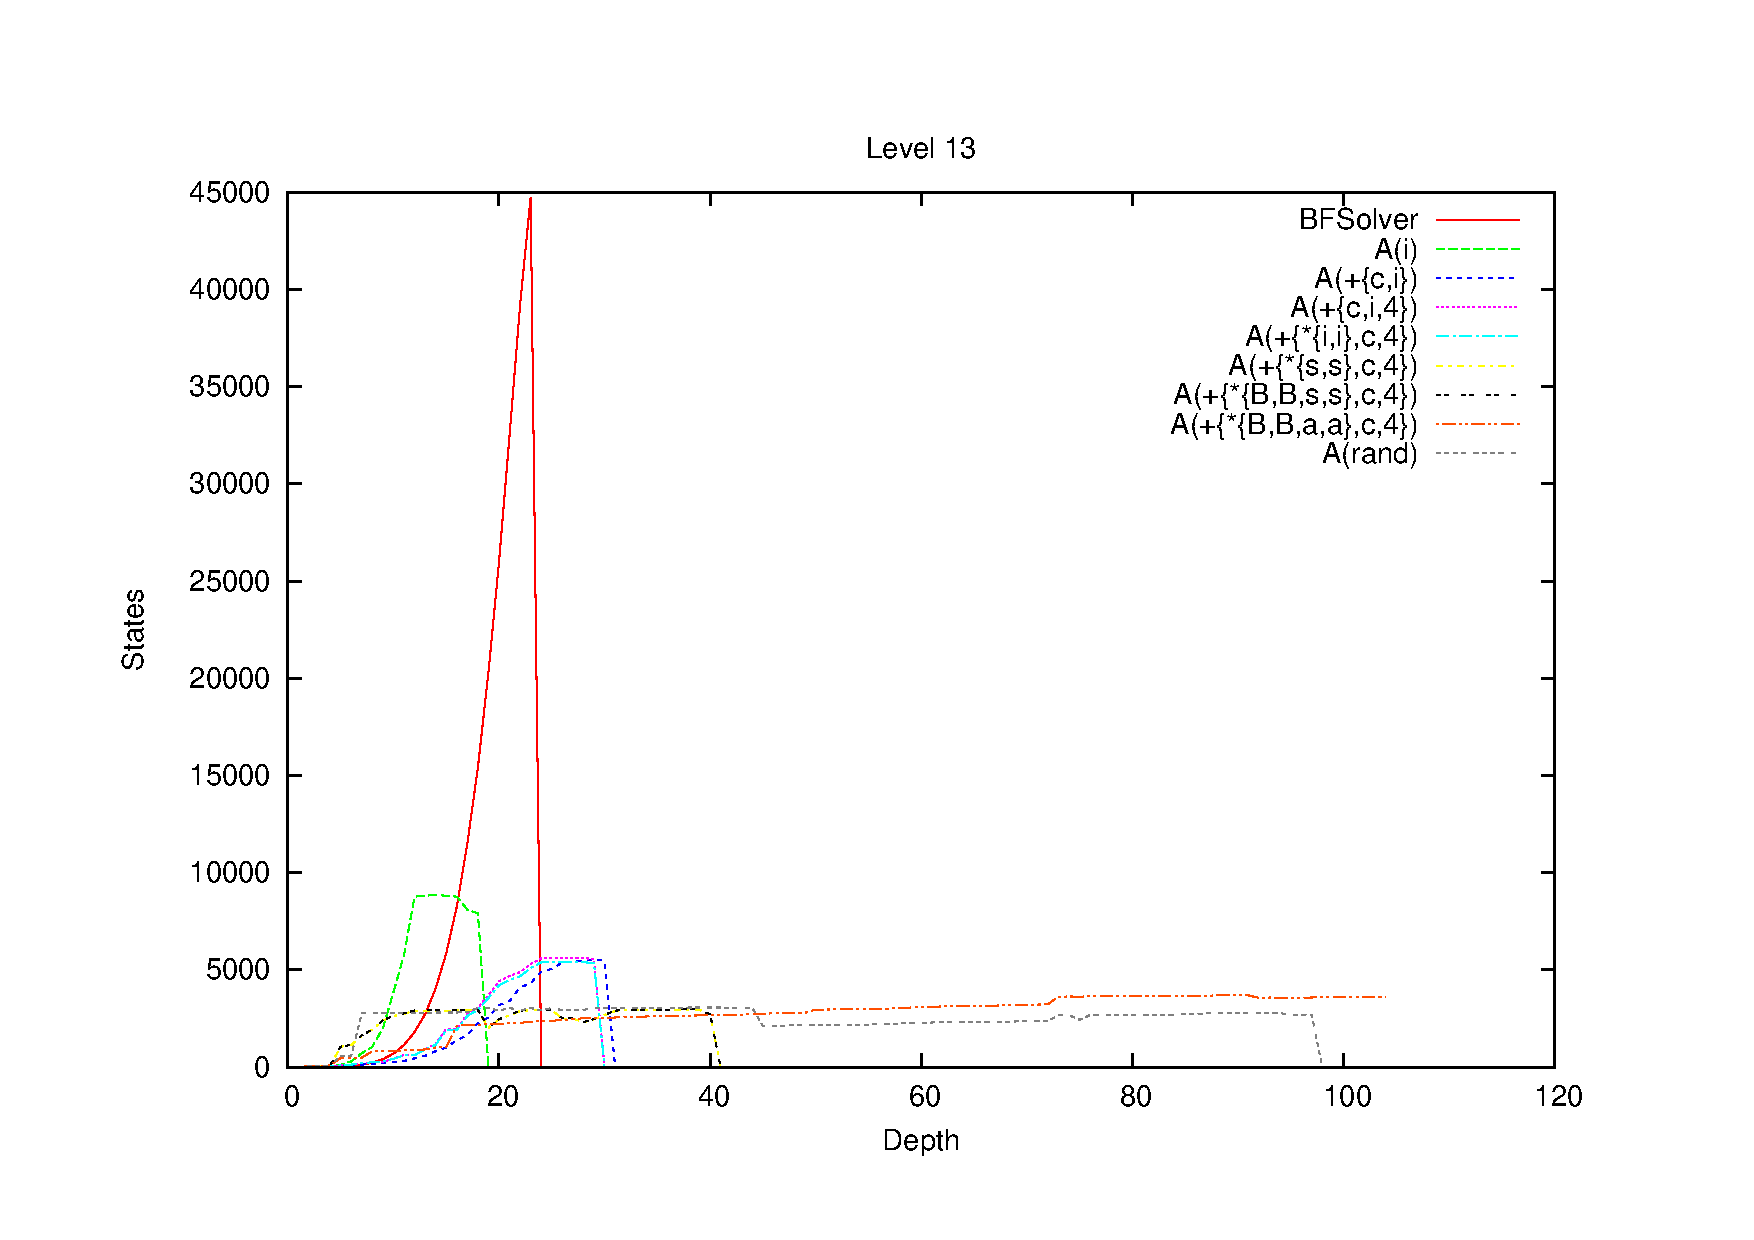
\includegraphics[width=0.85\textwidth]{level13-5}
  \caption{Level 13}
  \label{fig:level13-stats}
\end{figure}

\begin{figure}
  \centering
  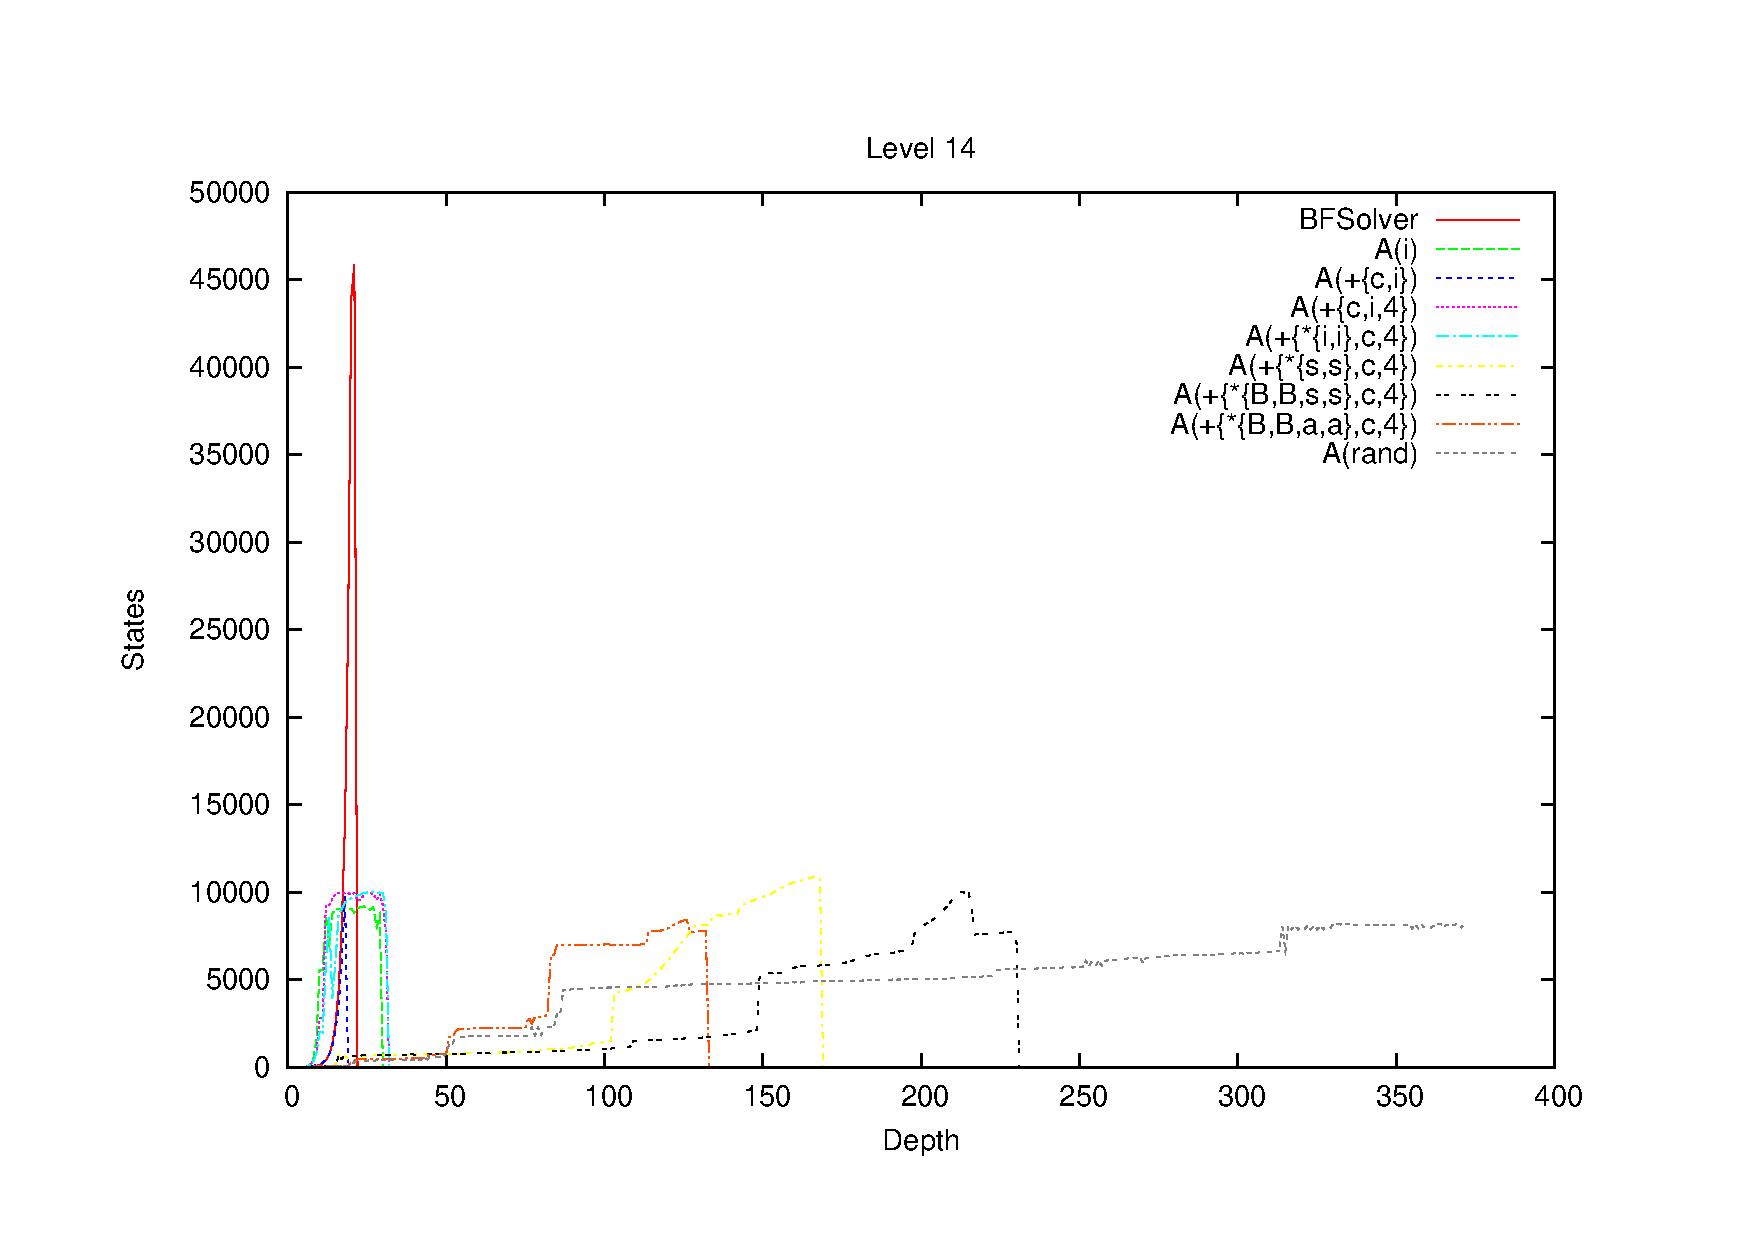
\includegraphics[width=0.85\textwidth]{level14-5}
  \caption{Level 14}
  \label{fig:level14-stats}
\end{figure}
 
\begin{figure}
  \centering
  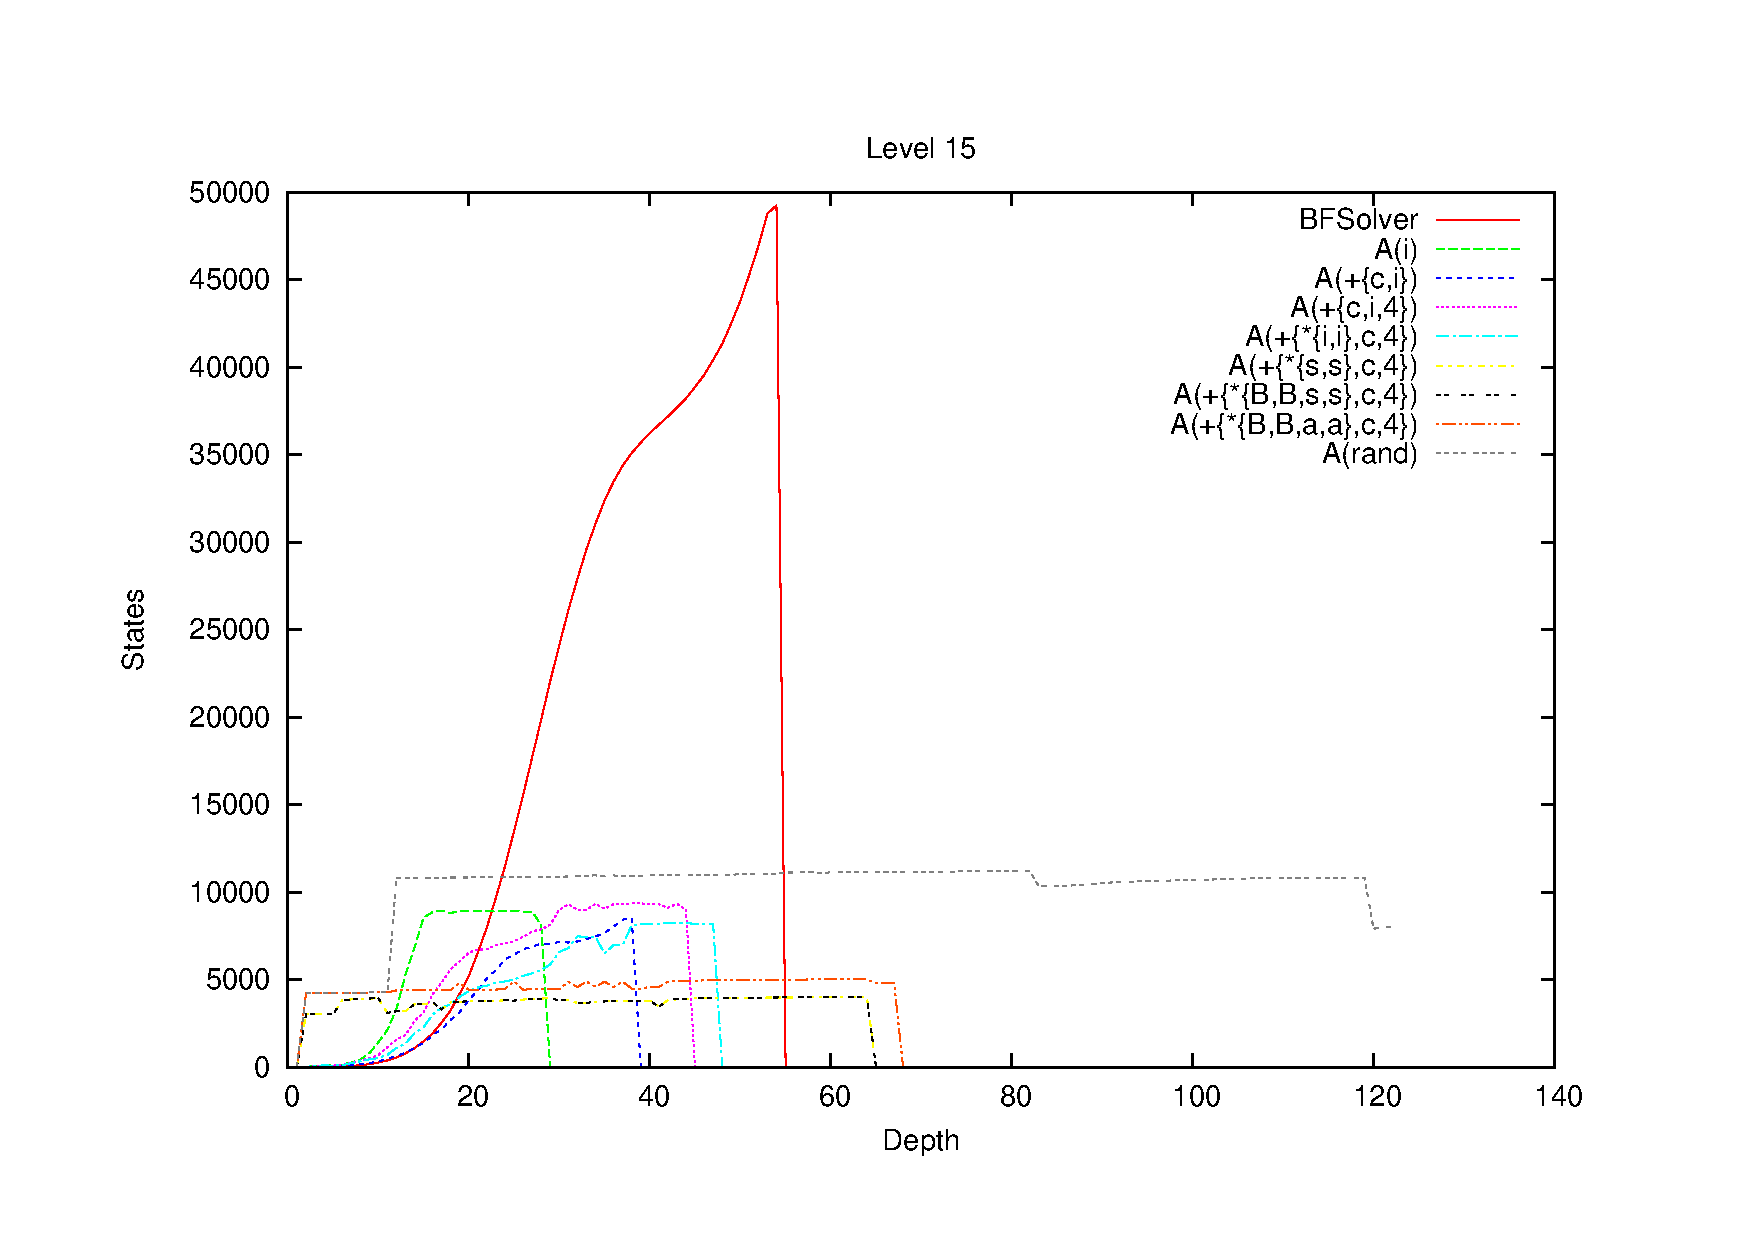
\includegraphics[width=0.85\textwidth]{level15-5}
  \caption{Level 15}
  \label{fig:level15-stats}
\end{figure}

\begin{figure}
  \centering
  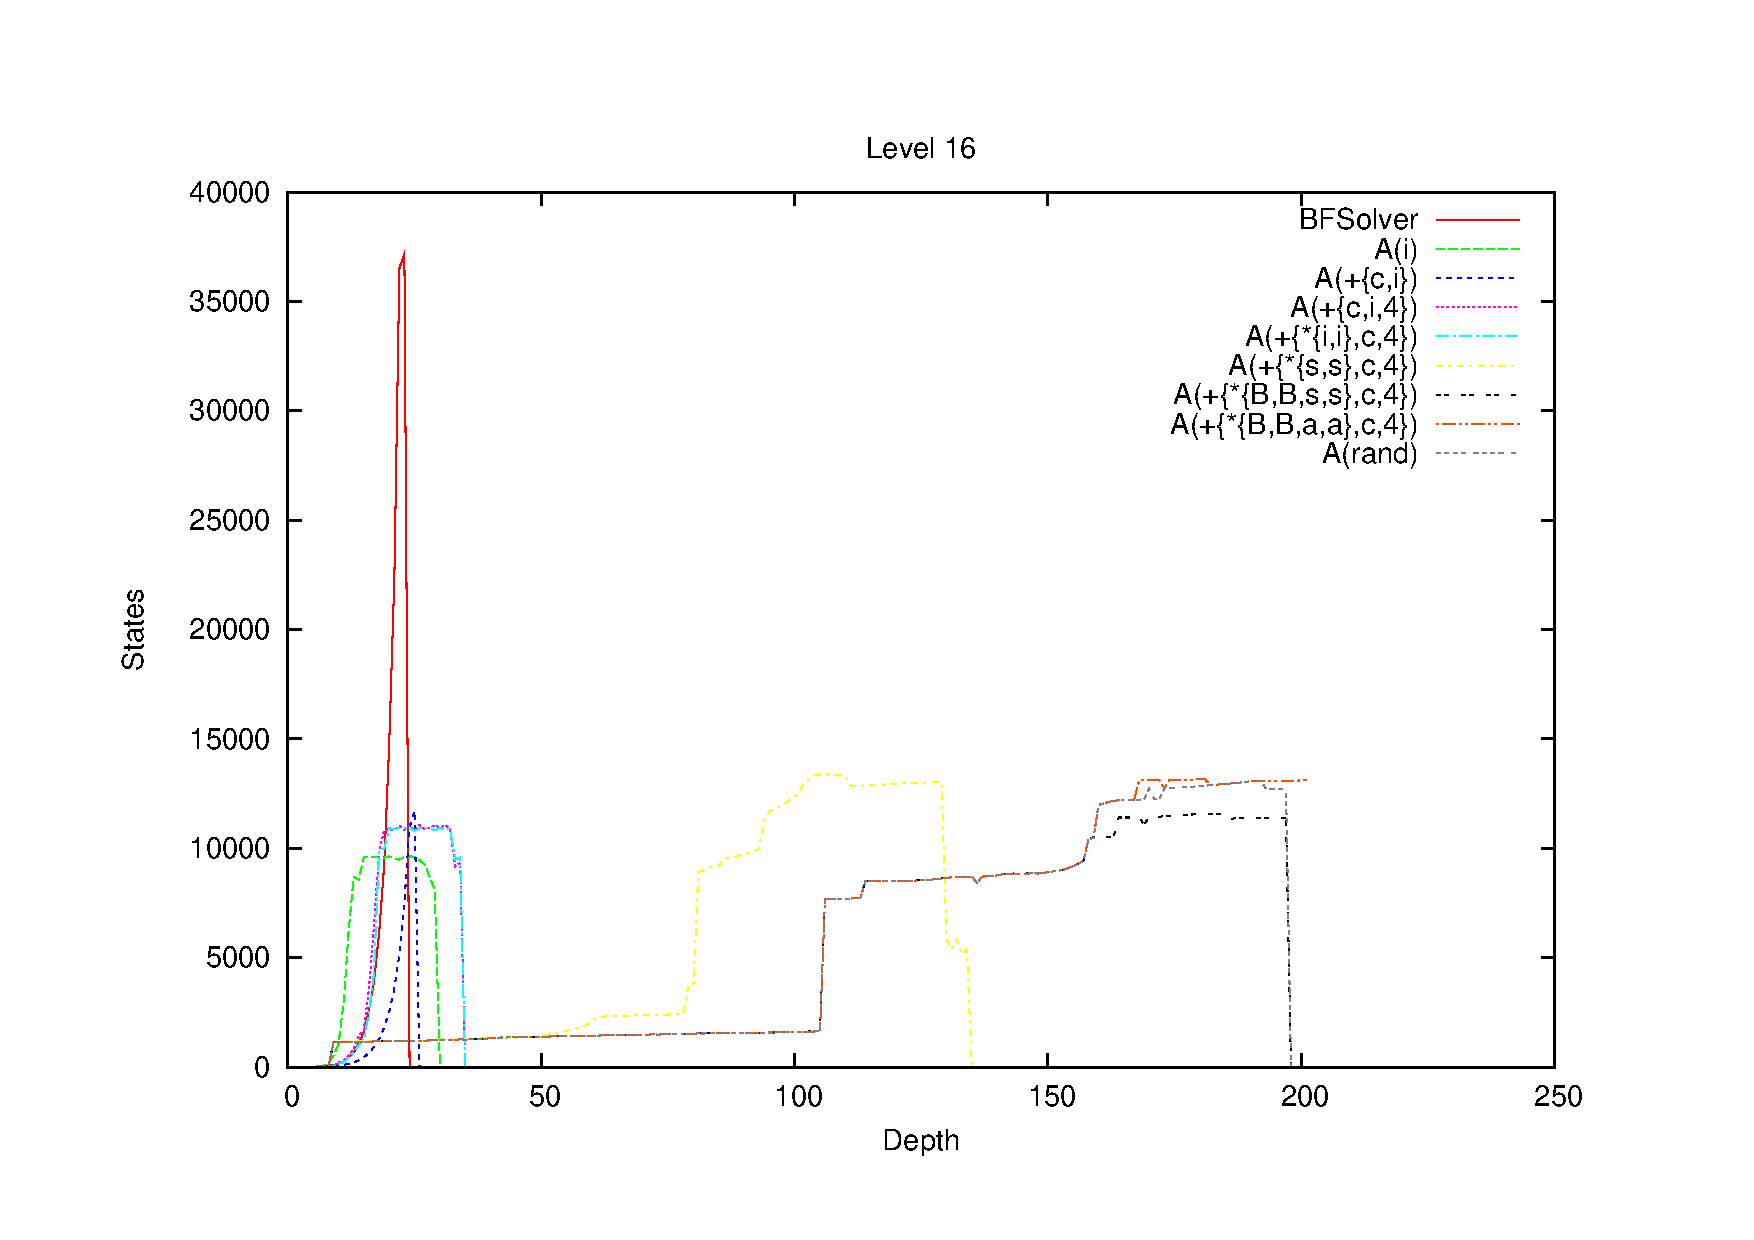
\includegraphics[width=0.85\textwidth]{level16-5}
  \caption{Level 16}
  \label{fig:level16-stats}
\end{figure}
 
\begin{figure}
  \centering
  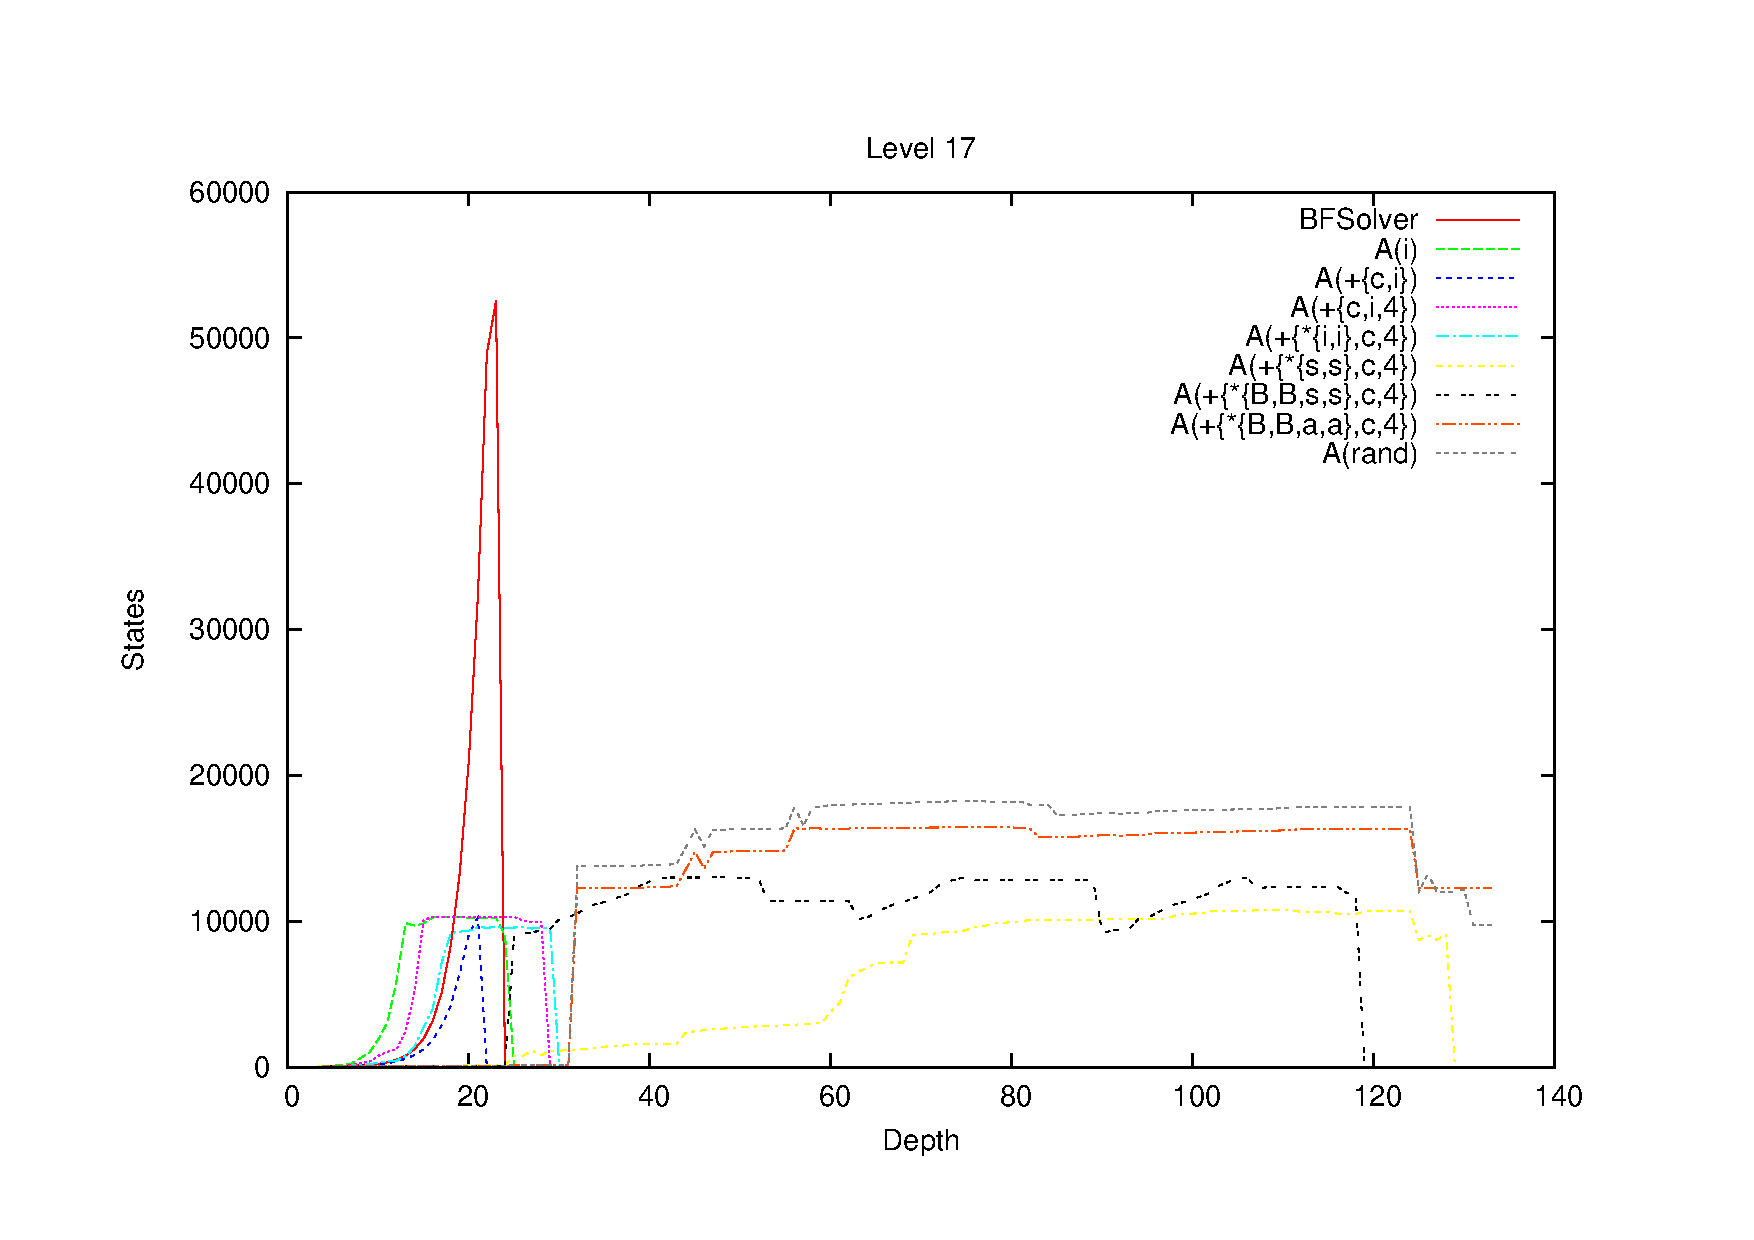
\includegraphics[width=0.85\textwidth]{level17-5}
  \caption{Level 17}
  \label{fig:level17-stats}
\end{figure}

\begin{figure}
  \centering
  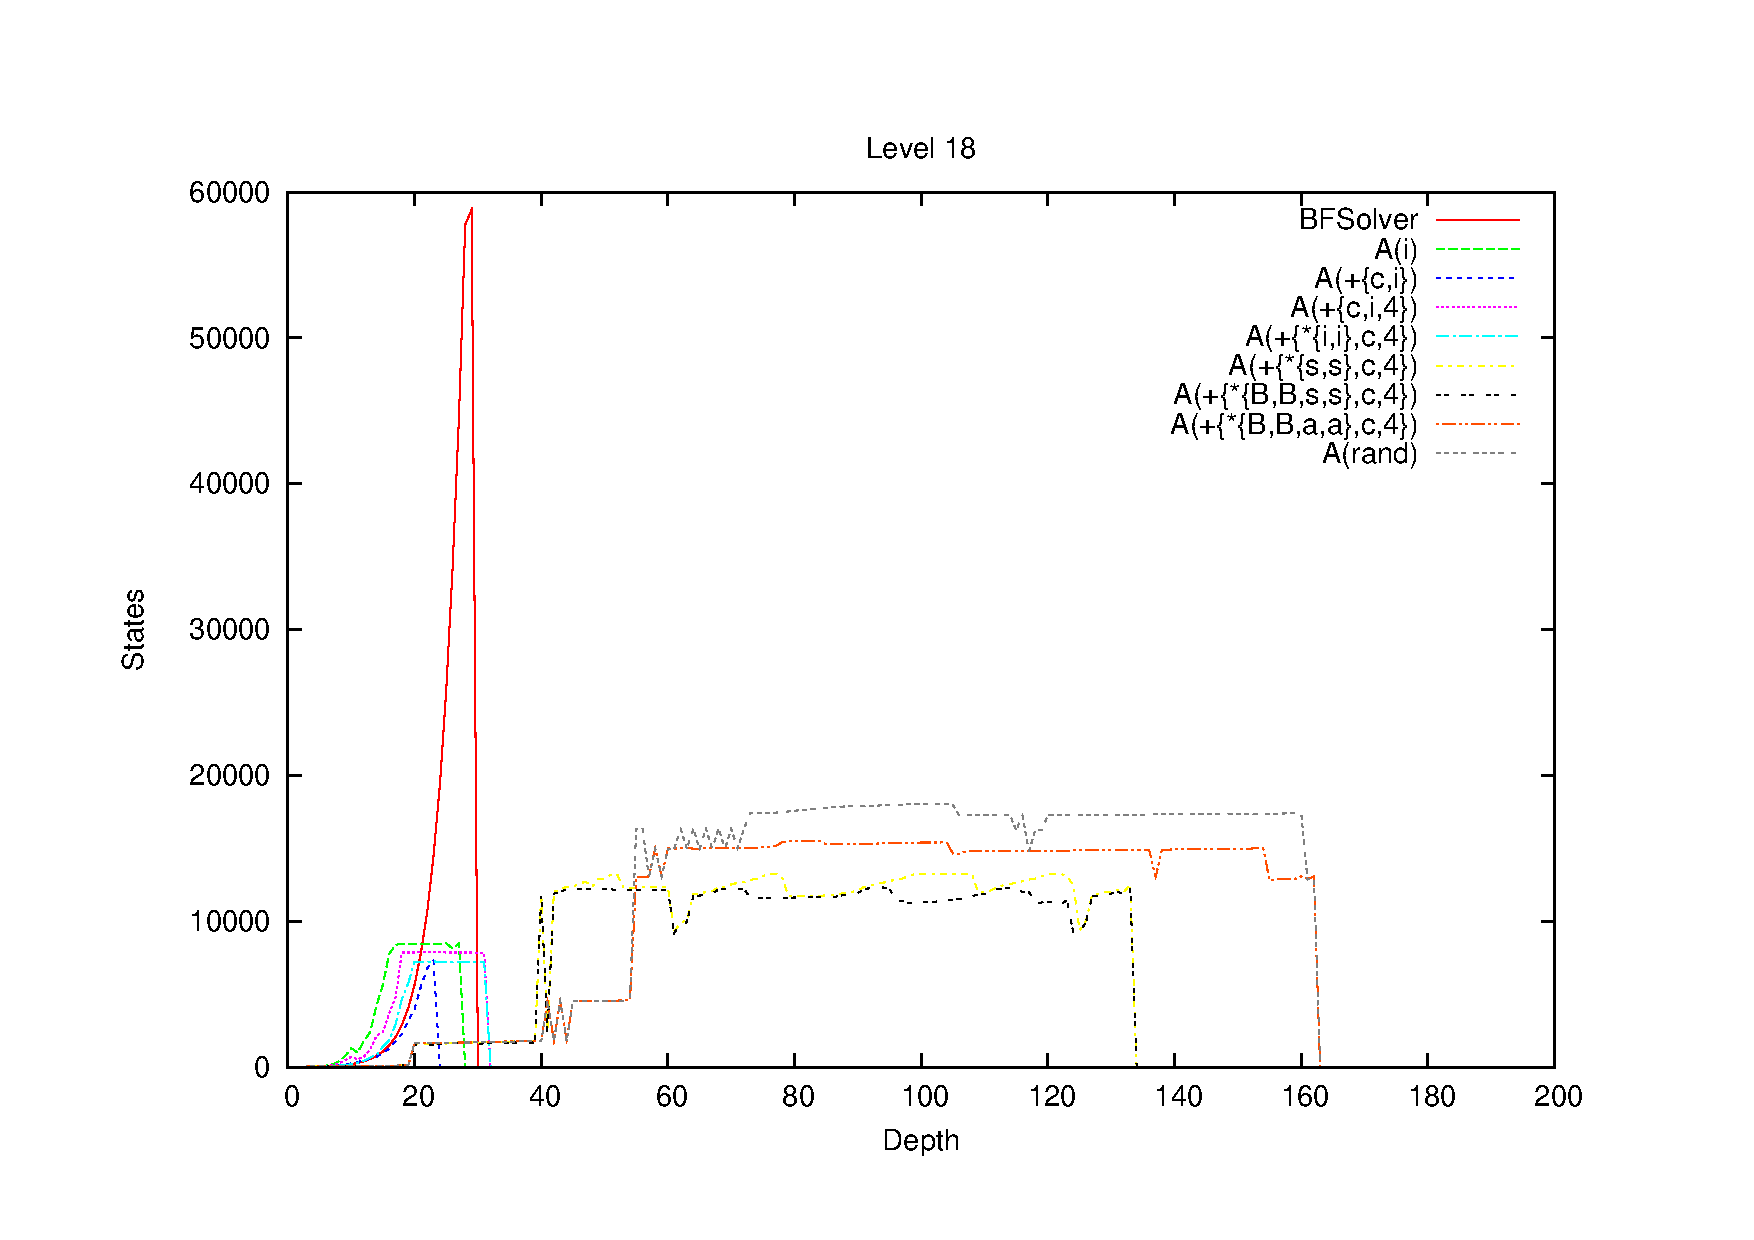
\includegraphics[width=0.85\textwidth]{level18-5}
  \caption{Level 18}
  \label{fig:level18-stats}
\end{figure}
 
\begin{figure}
  \centering
  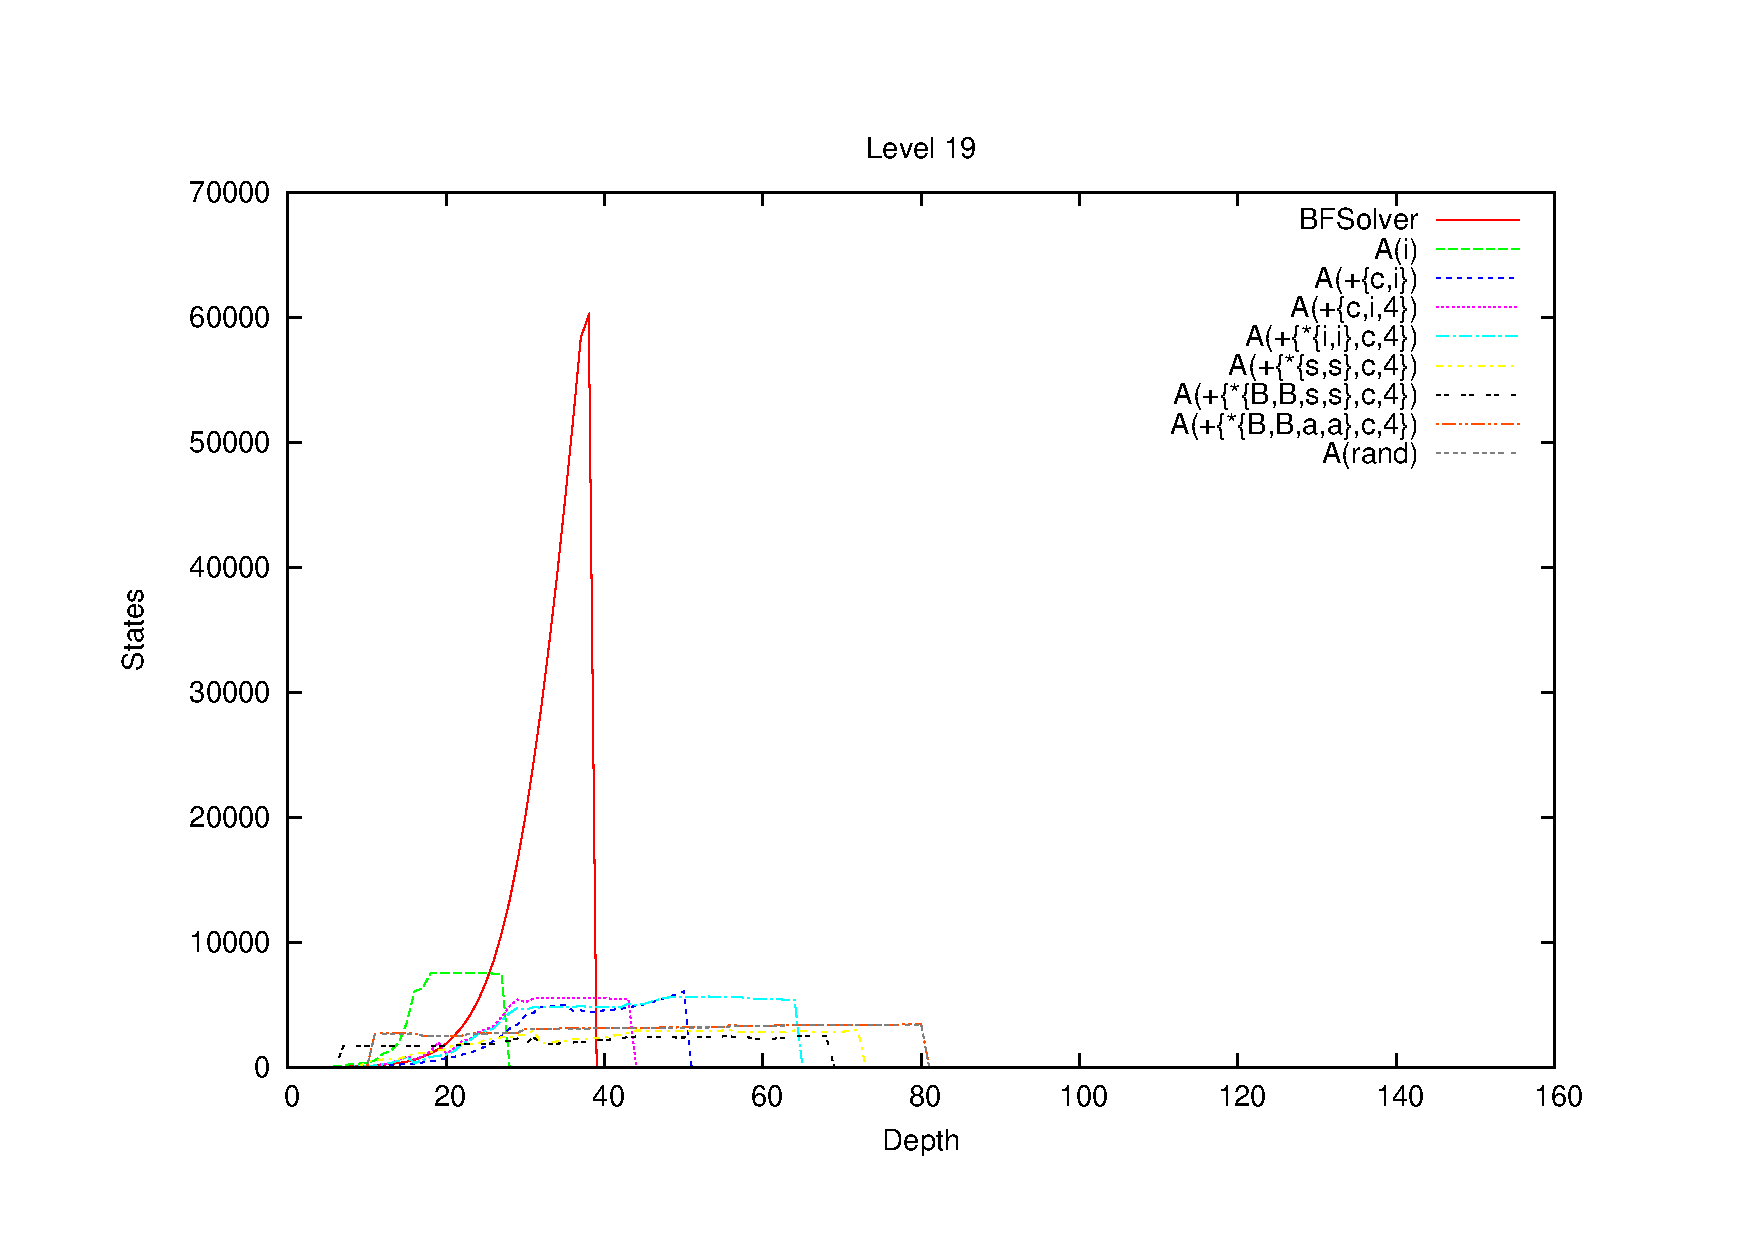
\includegraphics[width=0.85\textwidth]{level19-5}
  \caption{Level 19}
  \label{fig:level19-stats}
\end{figure}

\begin{figure}
  \centering
  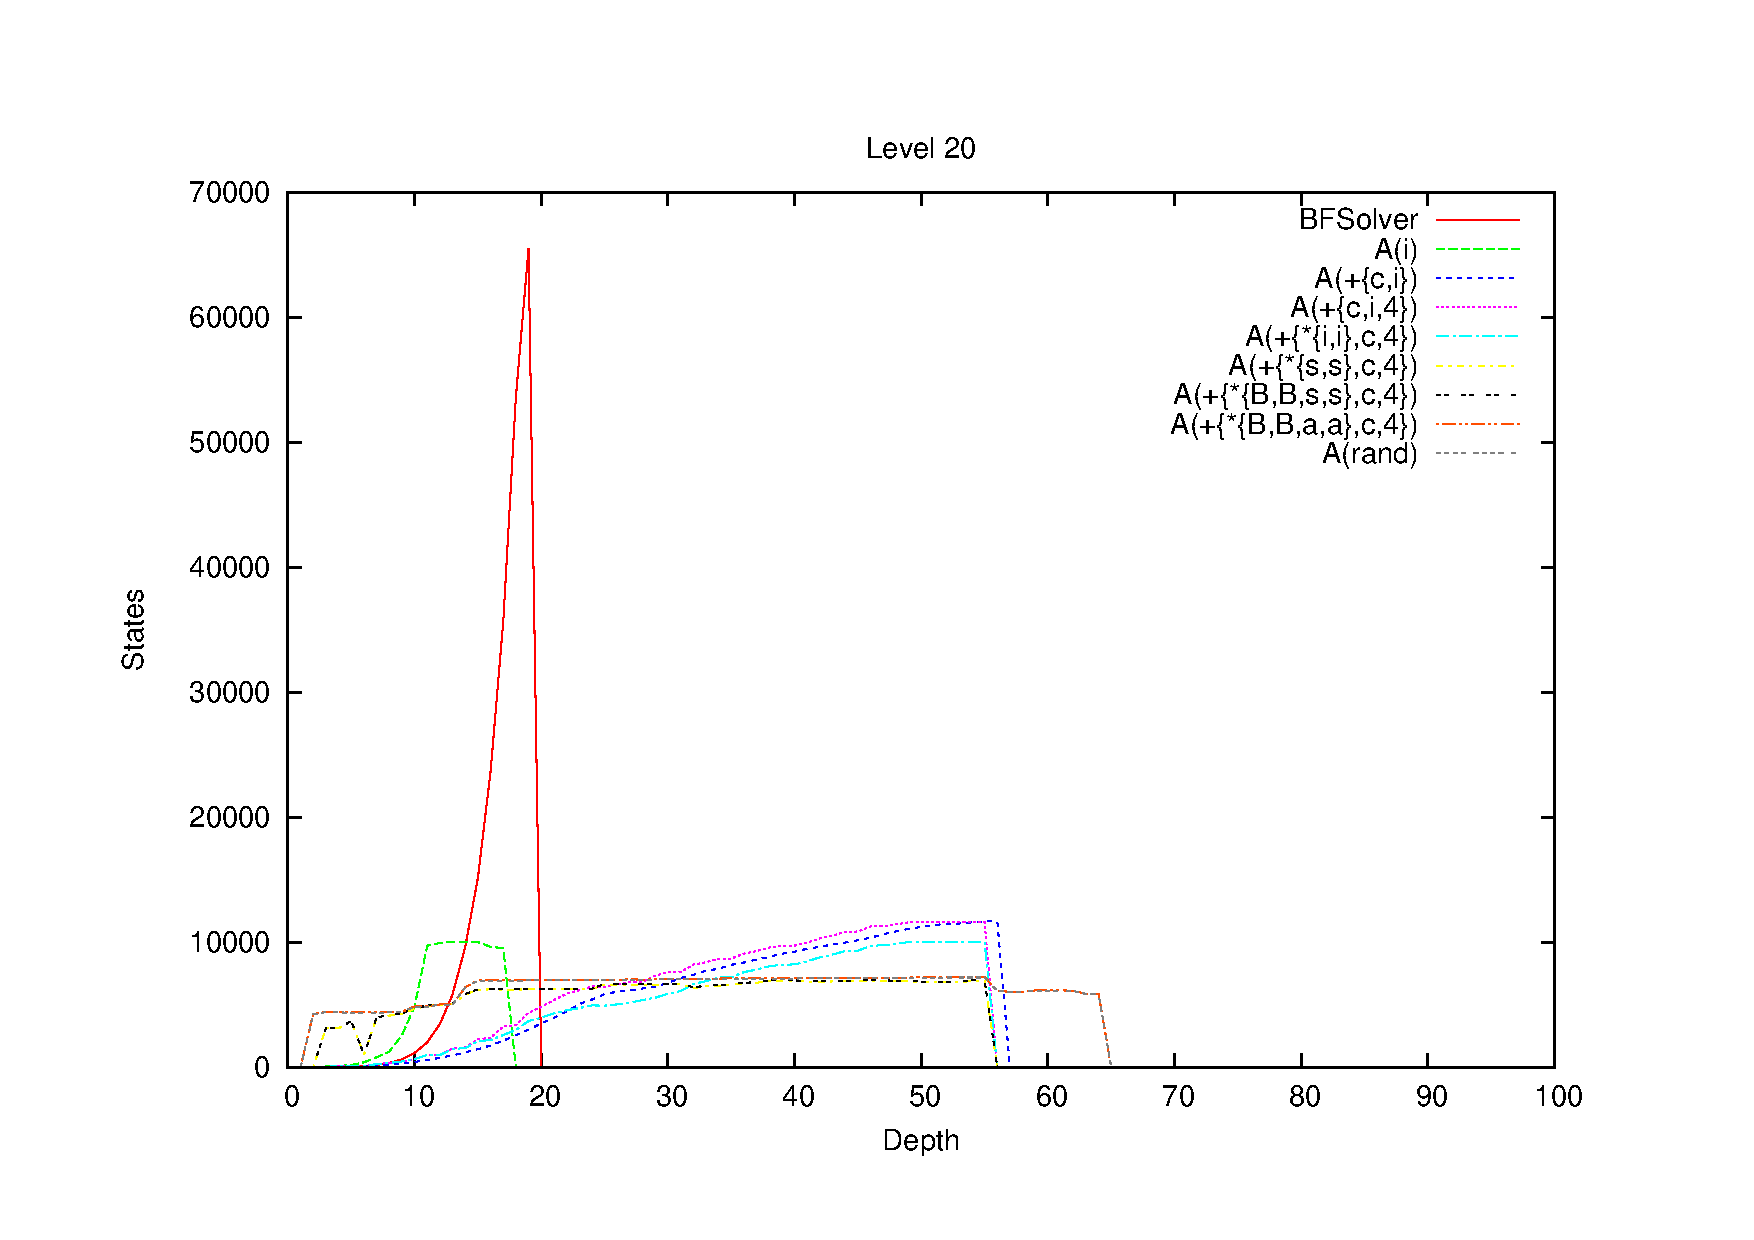
\includegraphics[width=0.85\textwidth]{level20-5}
  \caption{Level 20}
  \label{fig:level20-stats}
\end{figure}

\clearpage
 
\begin{figure}
  \centering
  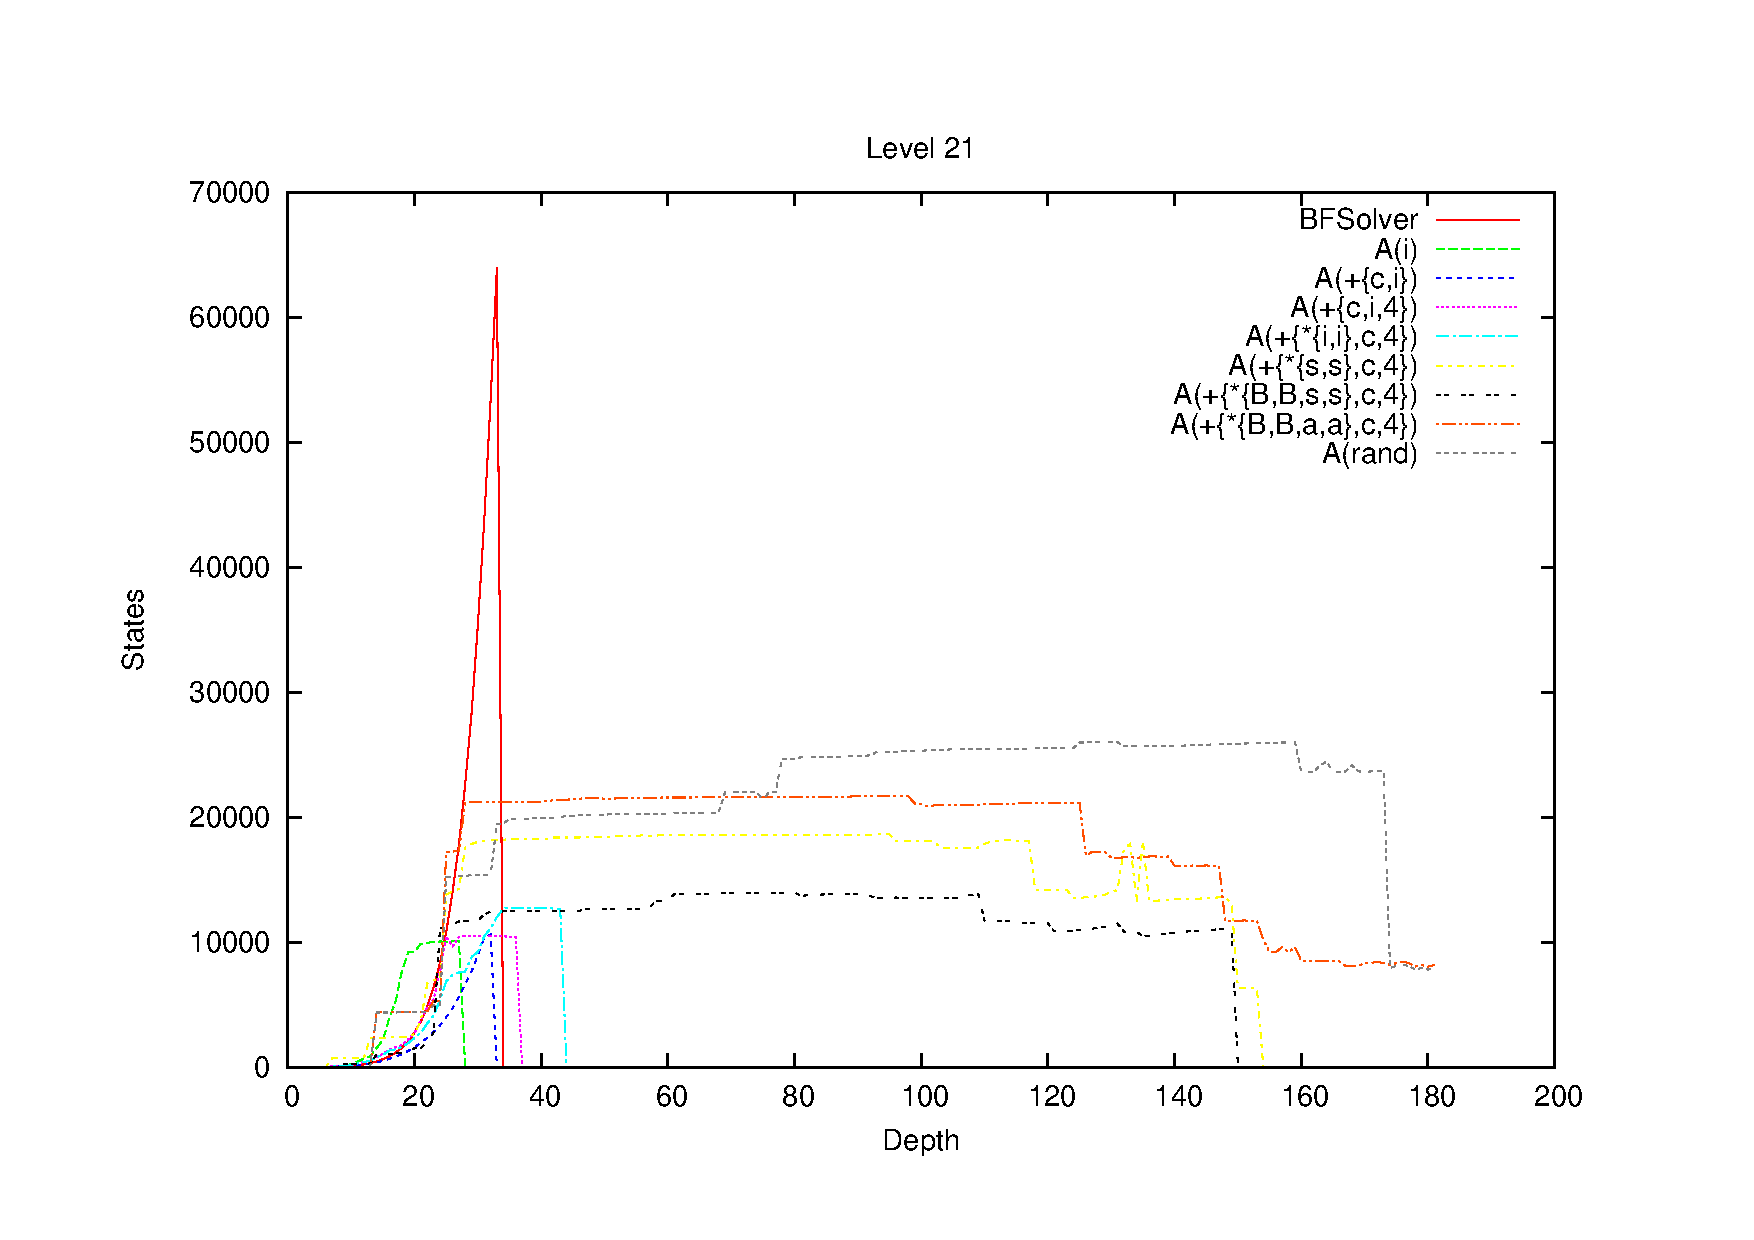
\includegraphics[width=0.85\textwidth]{level21-5}
  \caption{Level 21}
  \label{fig:level21-stats}
\end{figure}

\begin{figure}
  \centering
  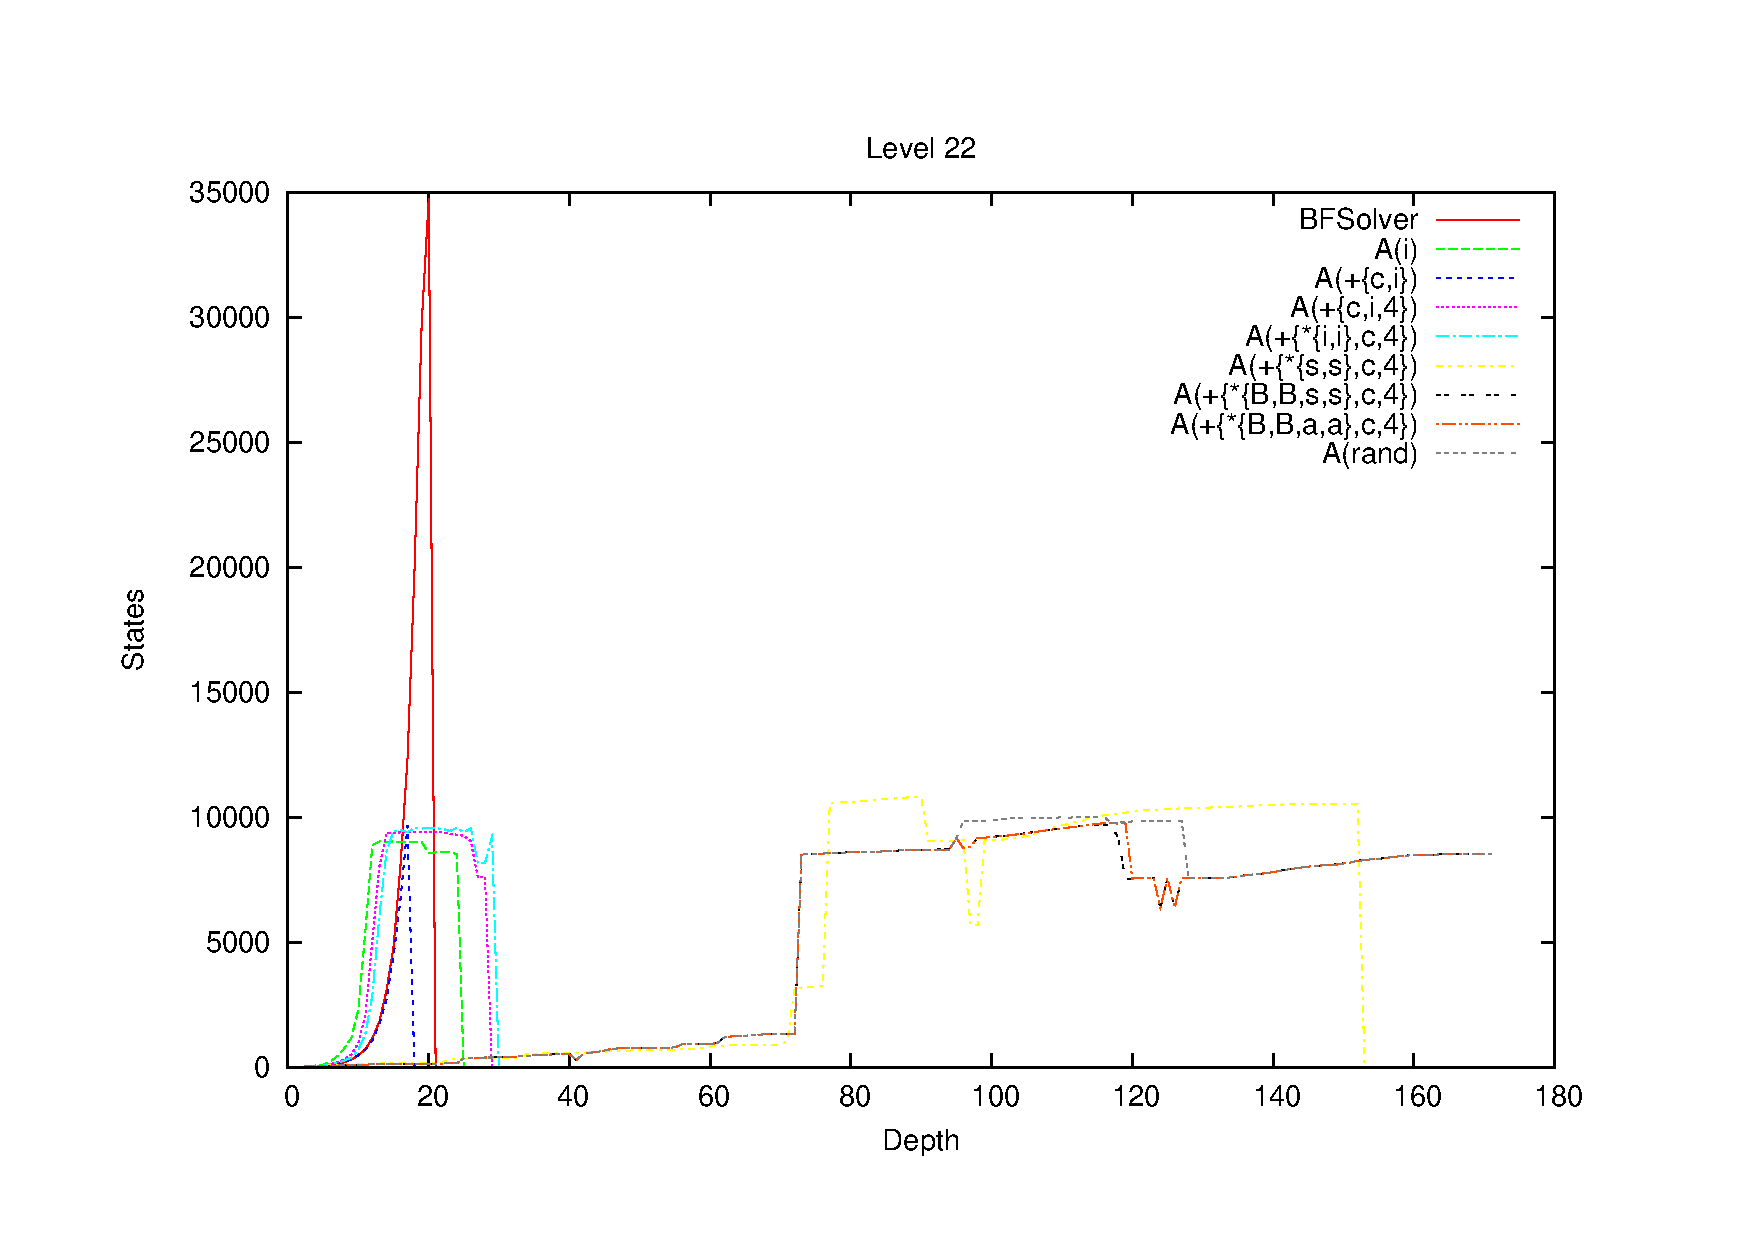
\includegraphics[width=0.85\textwidth]{level22-5}
  \caption{Level 22}
  \label{fig:level2-stats}
\end{figure}
 
\begin{figure}
  \centering
  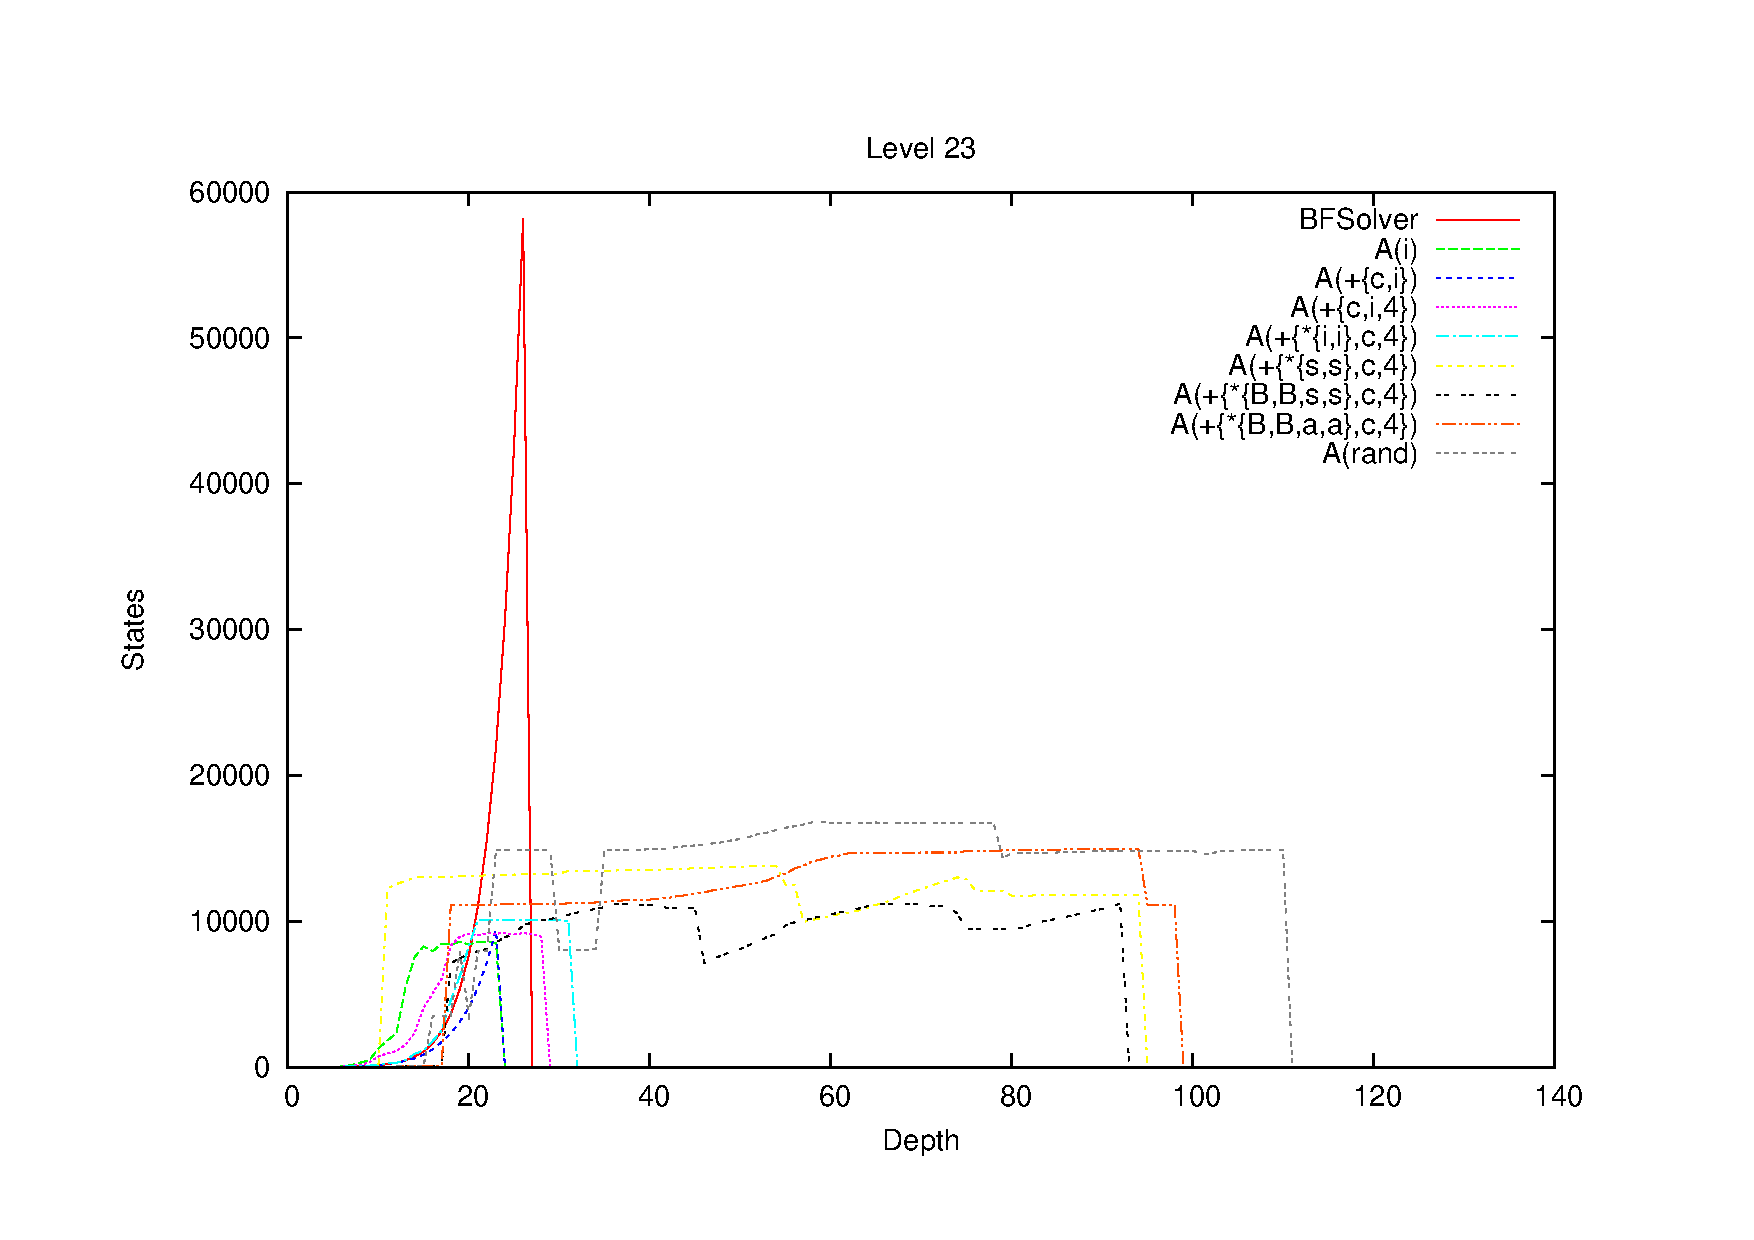
\includegraphics[width=0.85\textwidth]{level23-5}
  \caption{Level 23}
  \label{fig:level23-stats}
\end{figure}

\begin{figure}
  \centering
  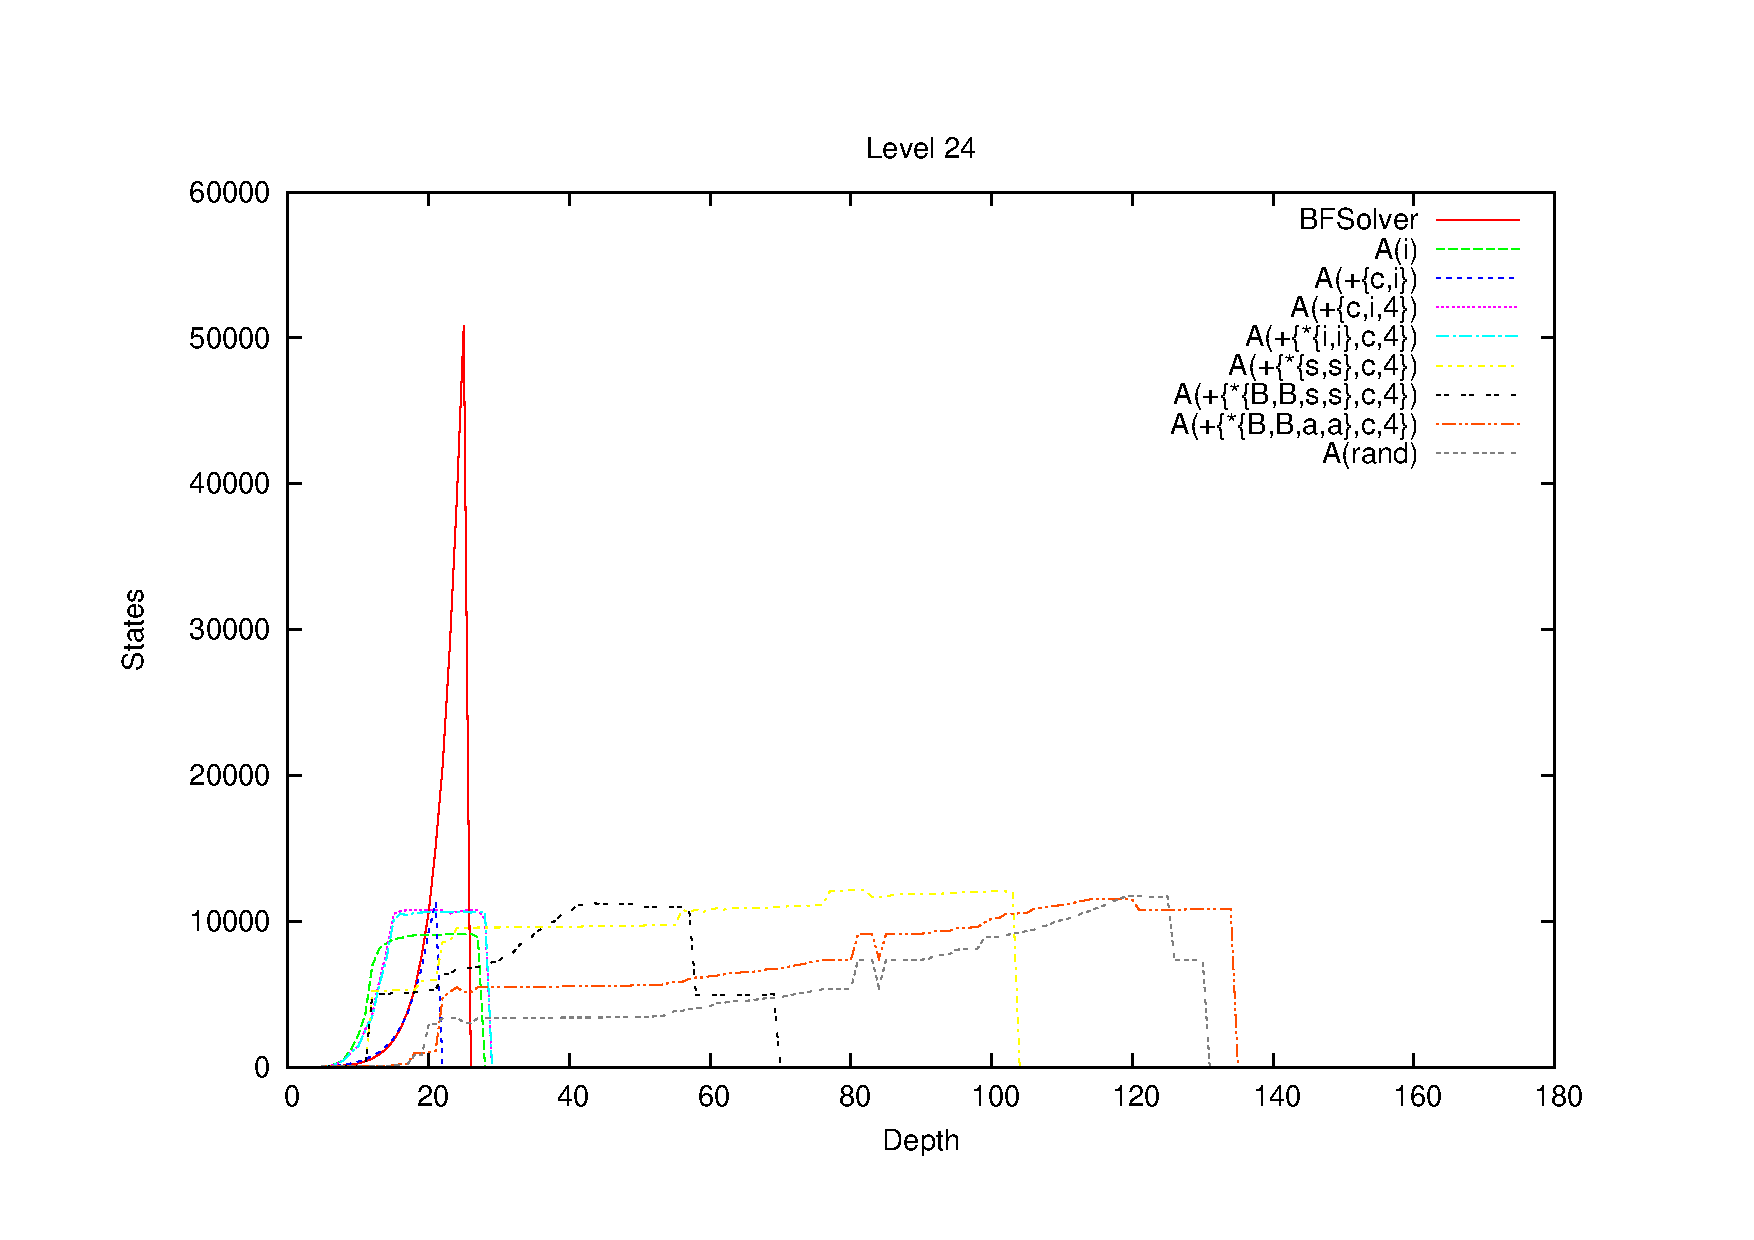
\includegraphics[width=0.85\textwidth]{level24-5}
  \caption{Level 24}
  \label{fig:level24-stats}
\end{figure}
 
\begin{figure}
  \centering
  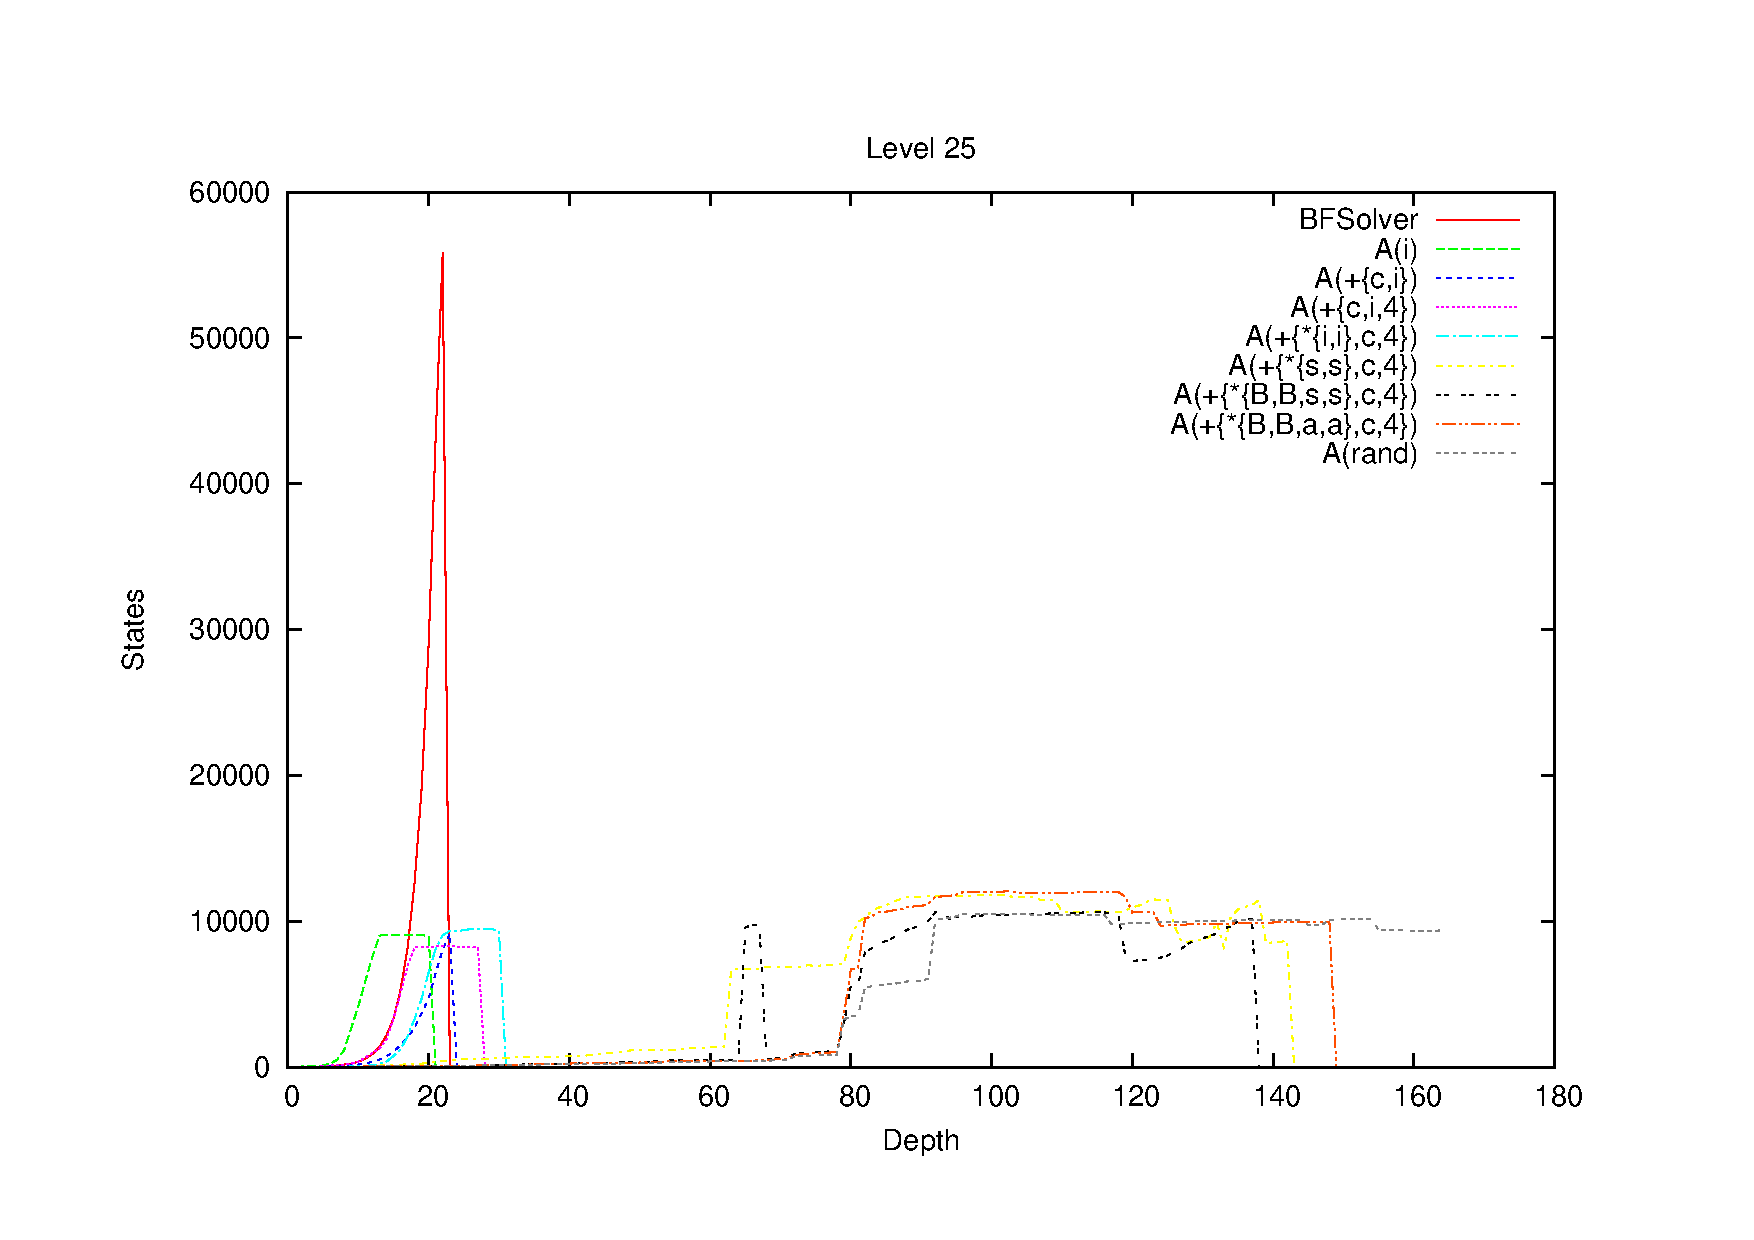
\includegraphics[width=0.85\textwidth]{level25-5}
  \caption{Level 25}
  \label{fig:level25-stats}
\end{figure}

\begin{figure}
  \centering
  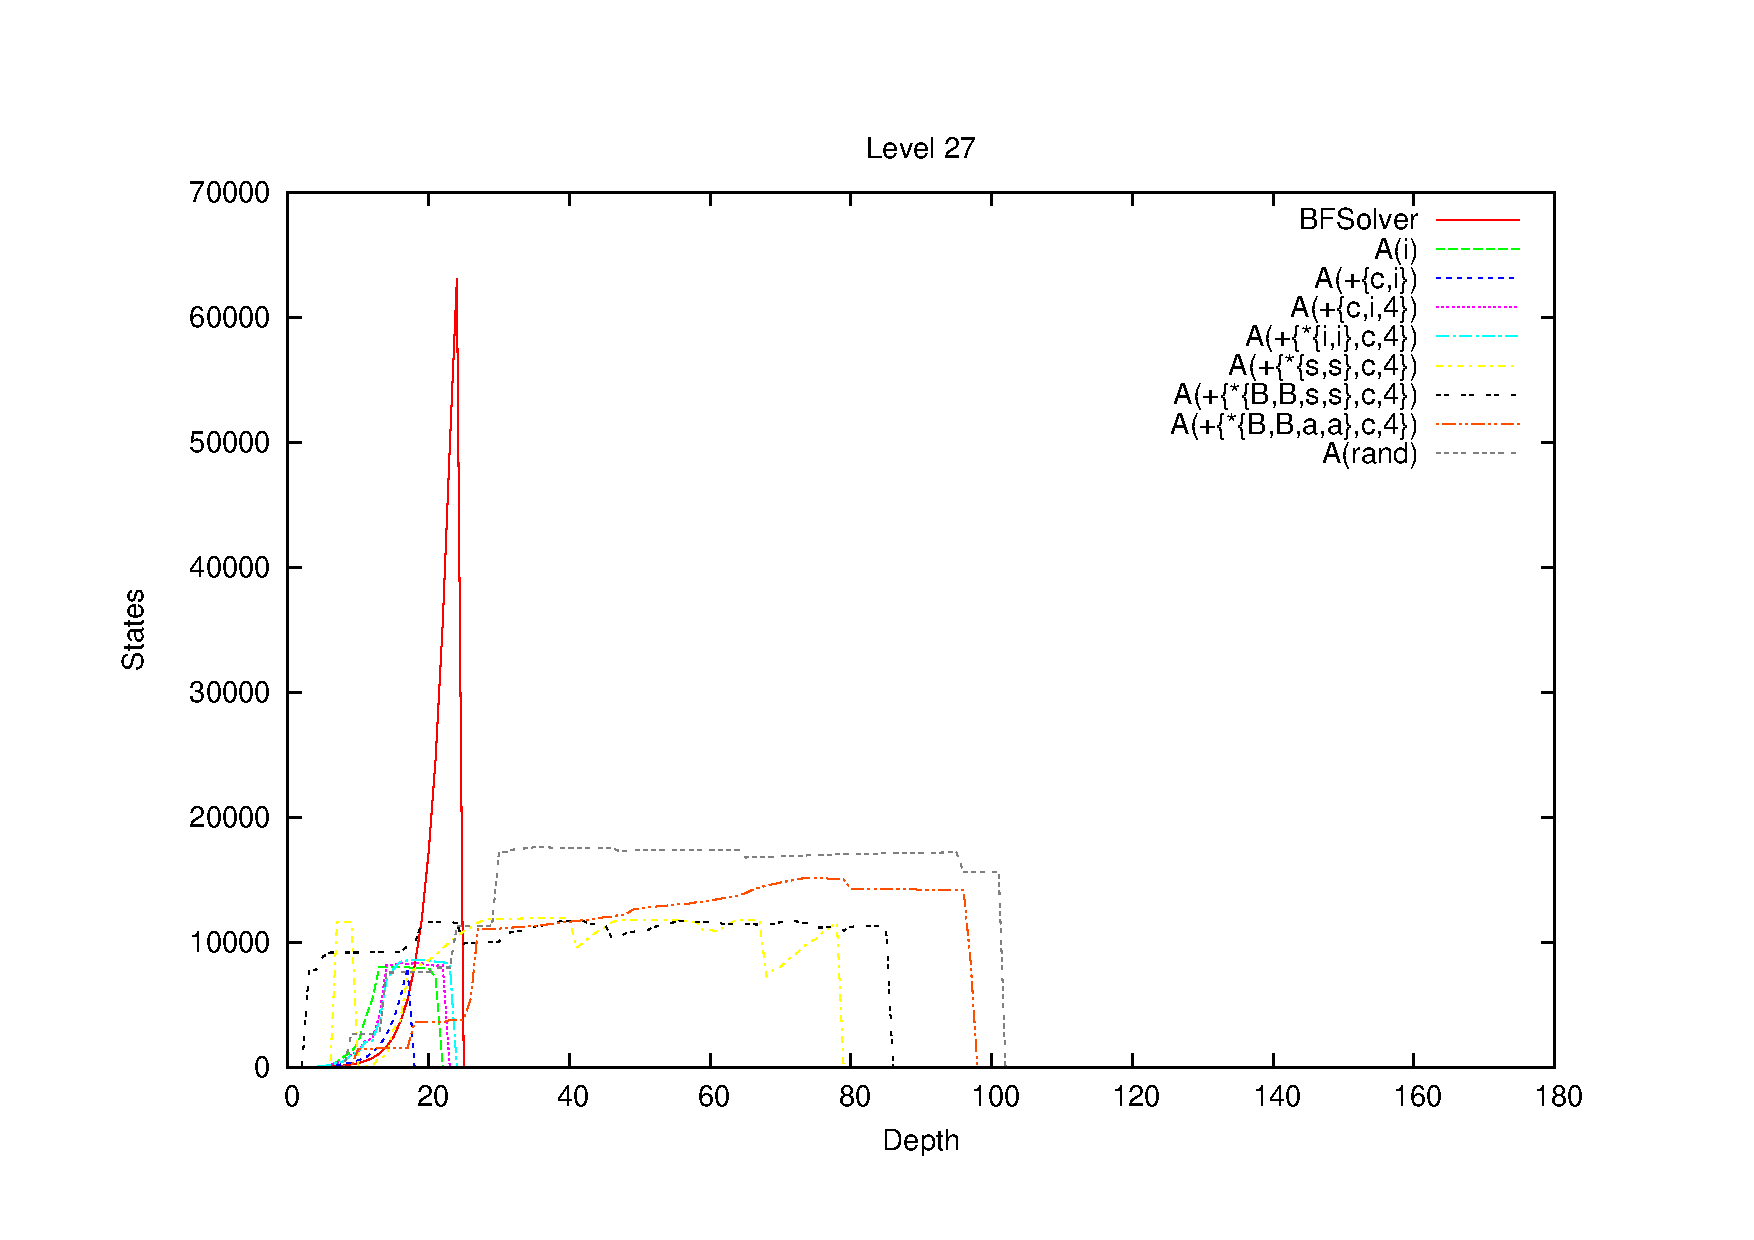
\includegraphics[width=0.85\textwidth]{level27-5}
  \caption{Level 27}
  \label{fig:level27-stats}
\end{figure}
 
\begin{figure}
  \centering
  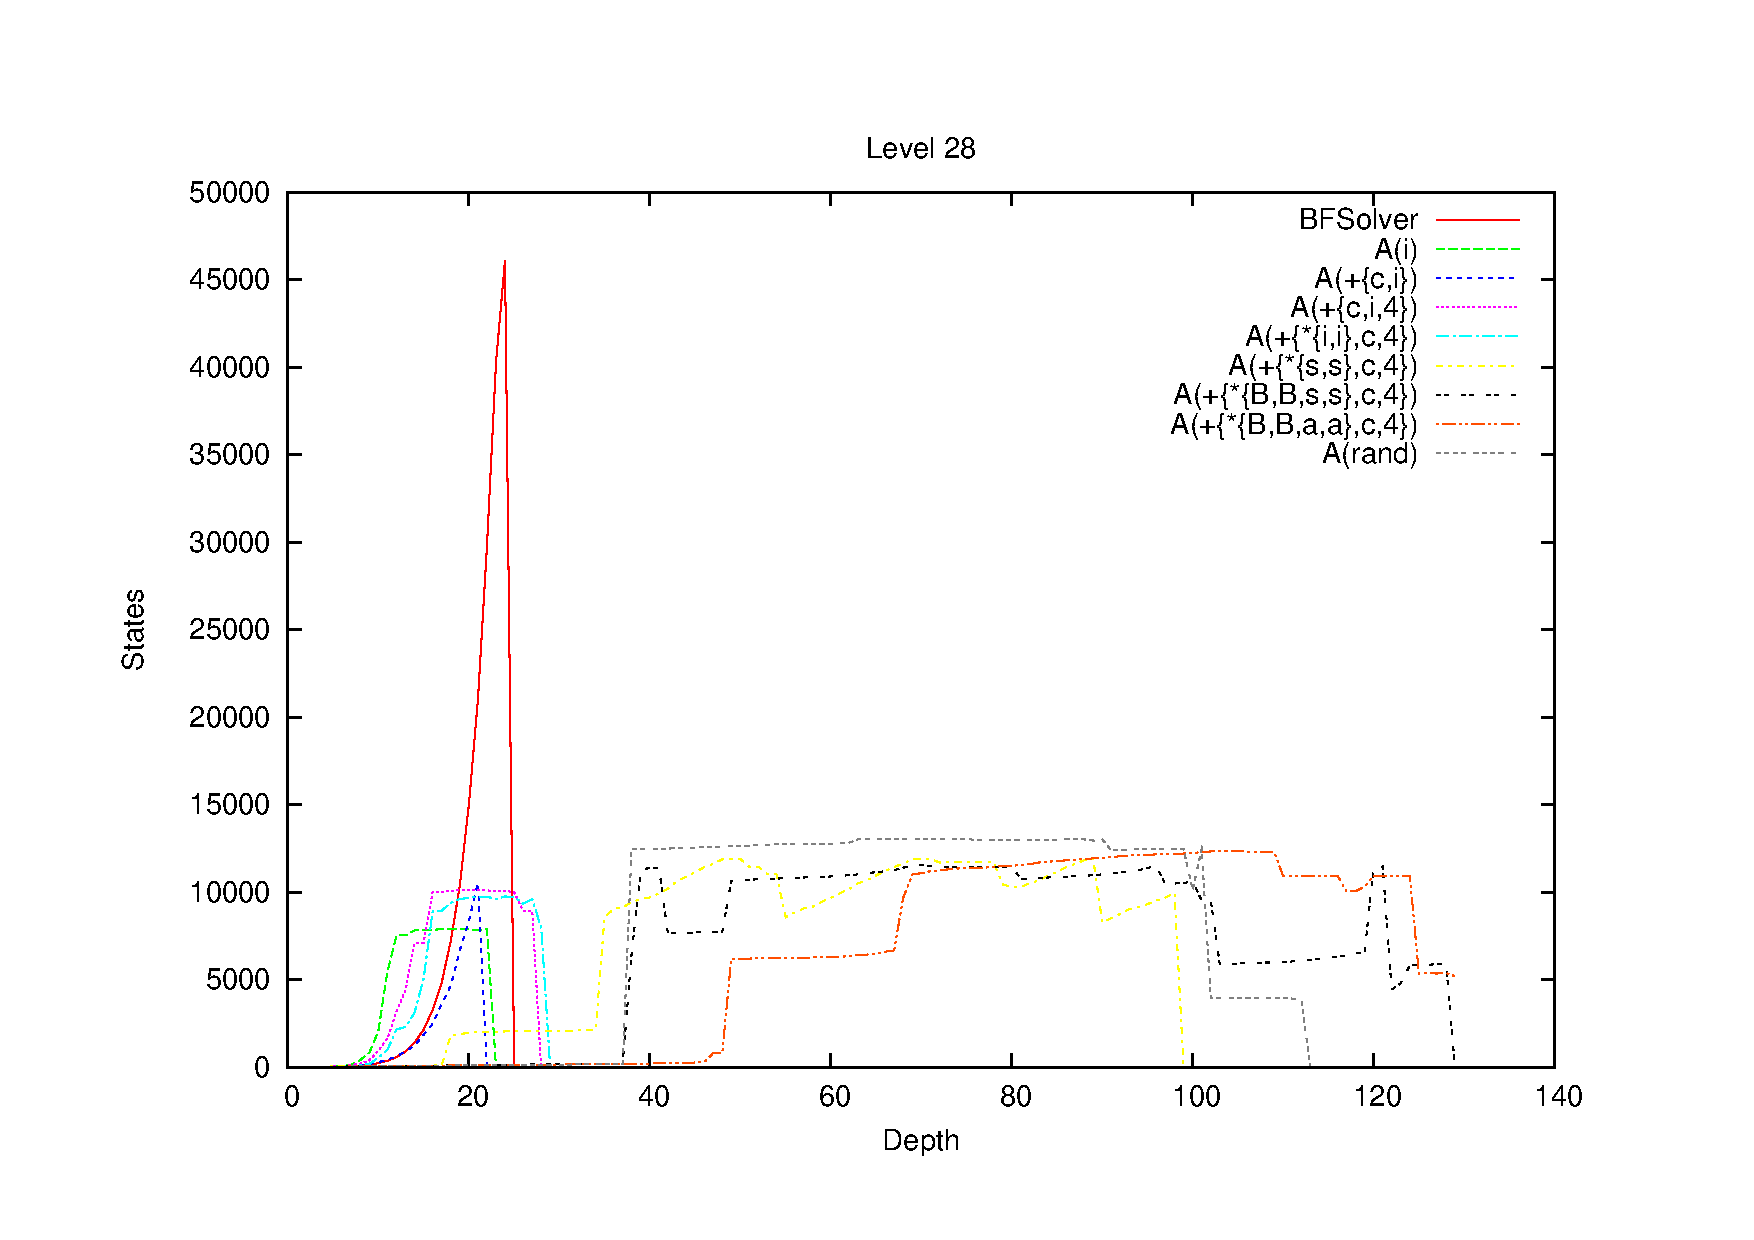
\includegraphics[width=0.85\textwidth]{level28-5}
  \caption{Level 28}
  \label{fig:level28-stats}
\end{figure}

\begin{figure}
  \centering
  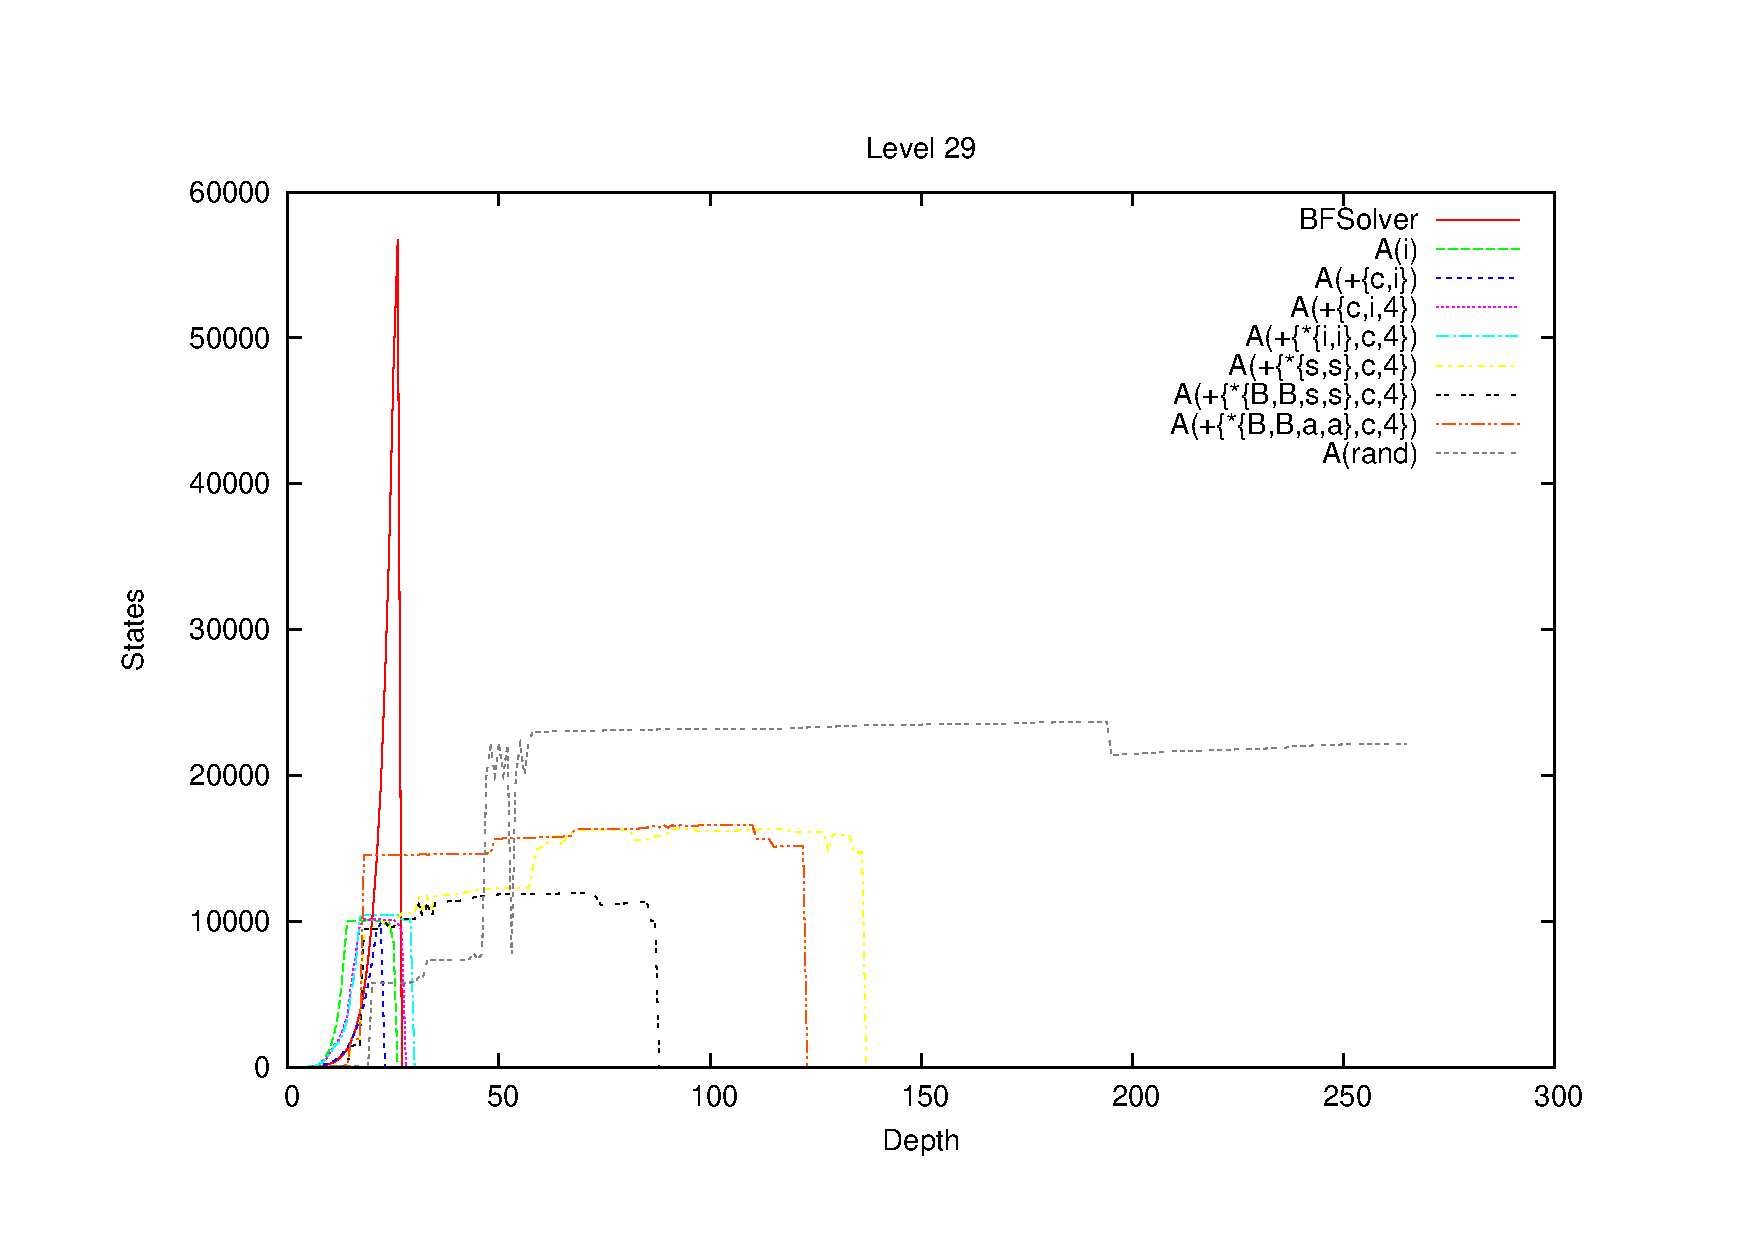
\includegraphics[width=0.85\textwidth]{level29-5}
  \caption{Level 29}
  \label{fig:level29-stats}
\end{figure}
 
\begin{figure}
  \centering
  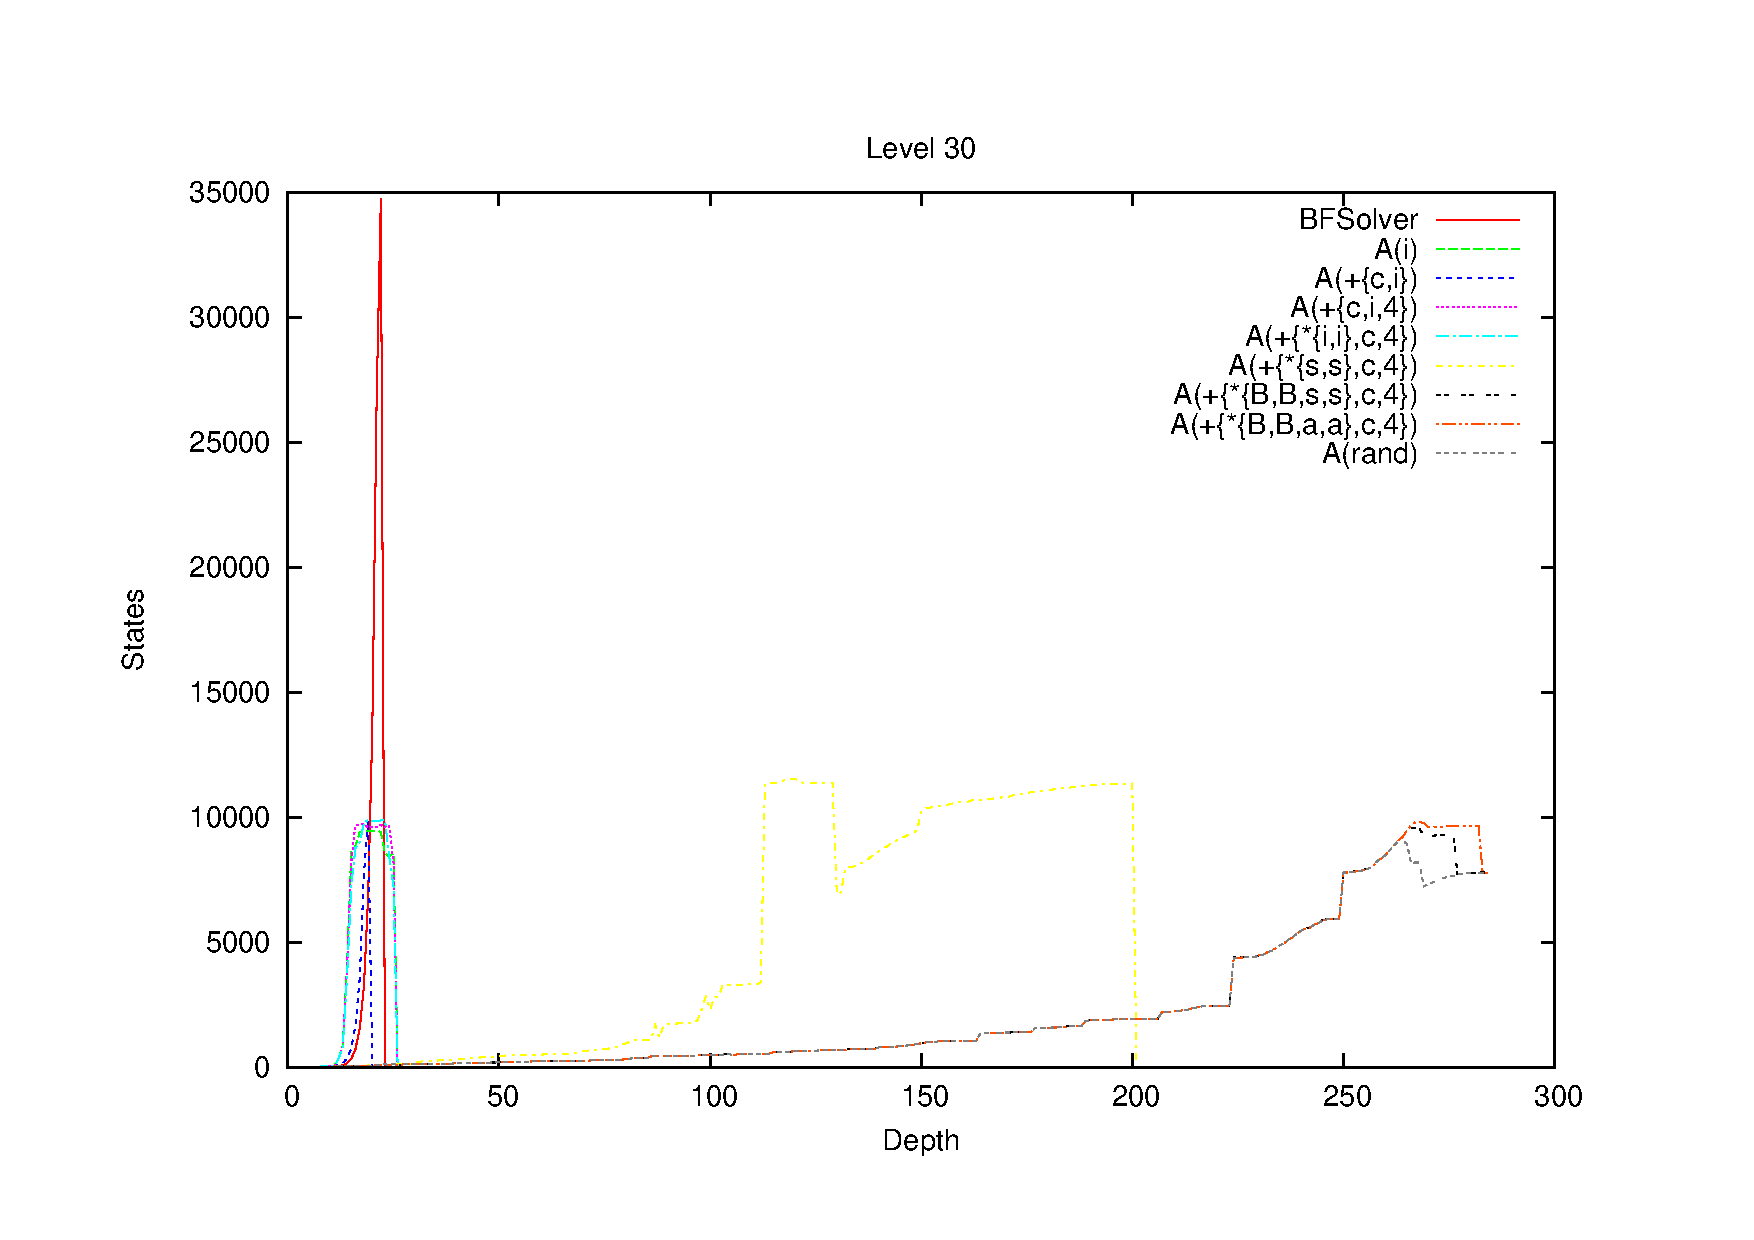
\includegraphics[width=0.85\textwidth]{level30-5}
  \caption{Level 30}
  \label{fig:level30-stats}
\end{figure}

\clearpage

\begin{figure}
  \centering
  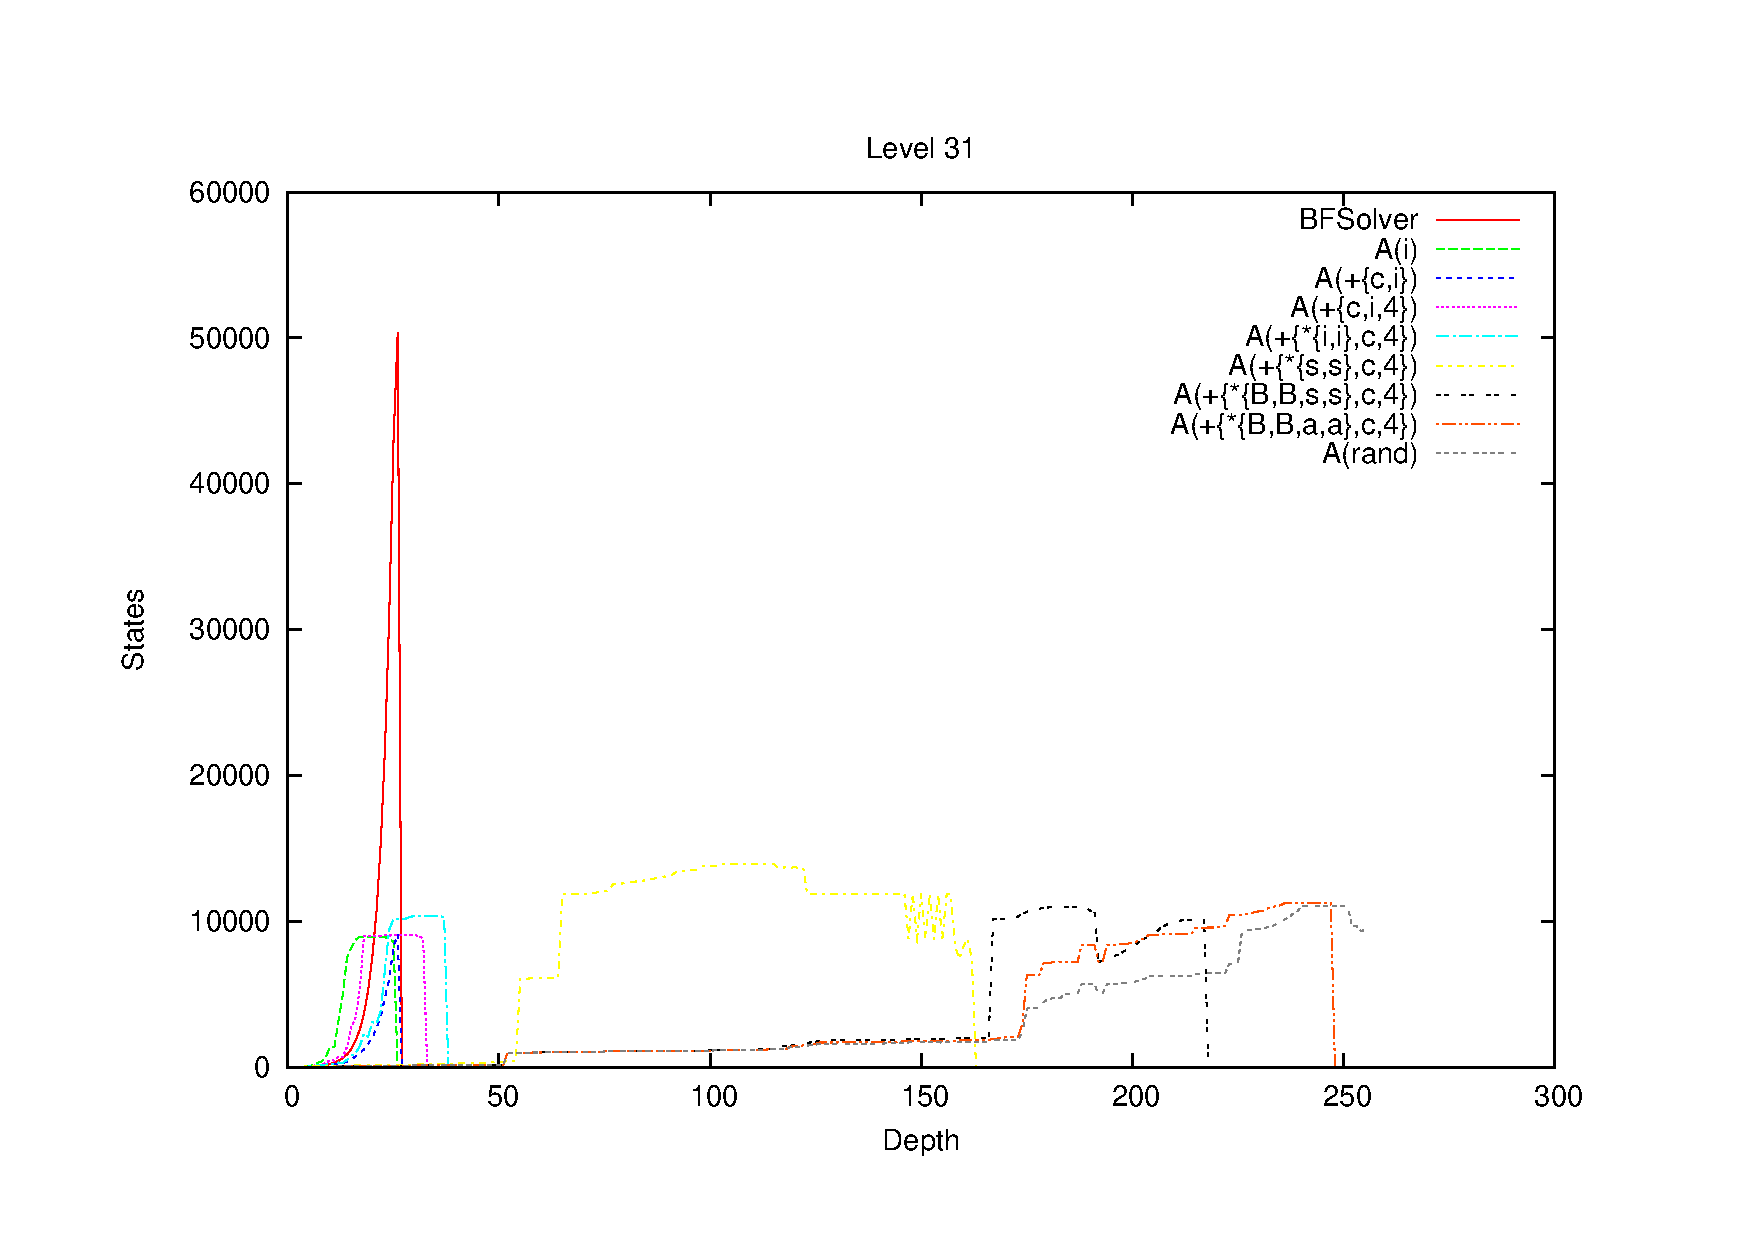
\includegraphics[width=0.85\textwidth]{level31-5}
  \caption{Level 31}
  \label{fig:level31-stats}
\end{figure}
 
\begin{figure}
  \centering
  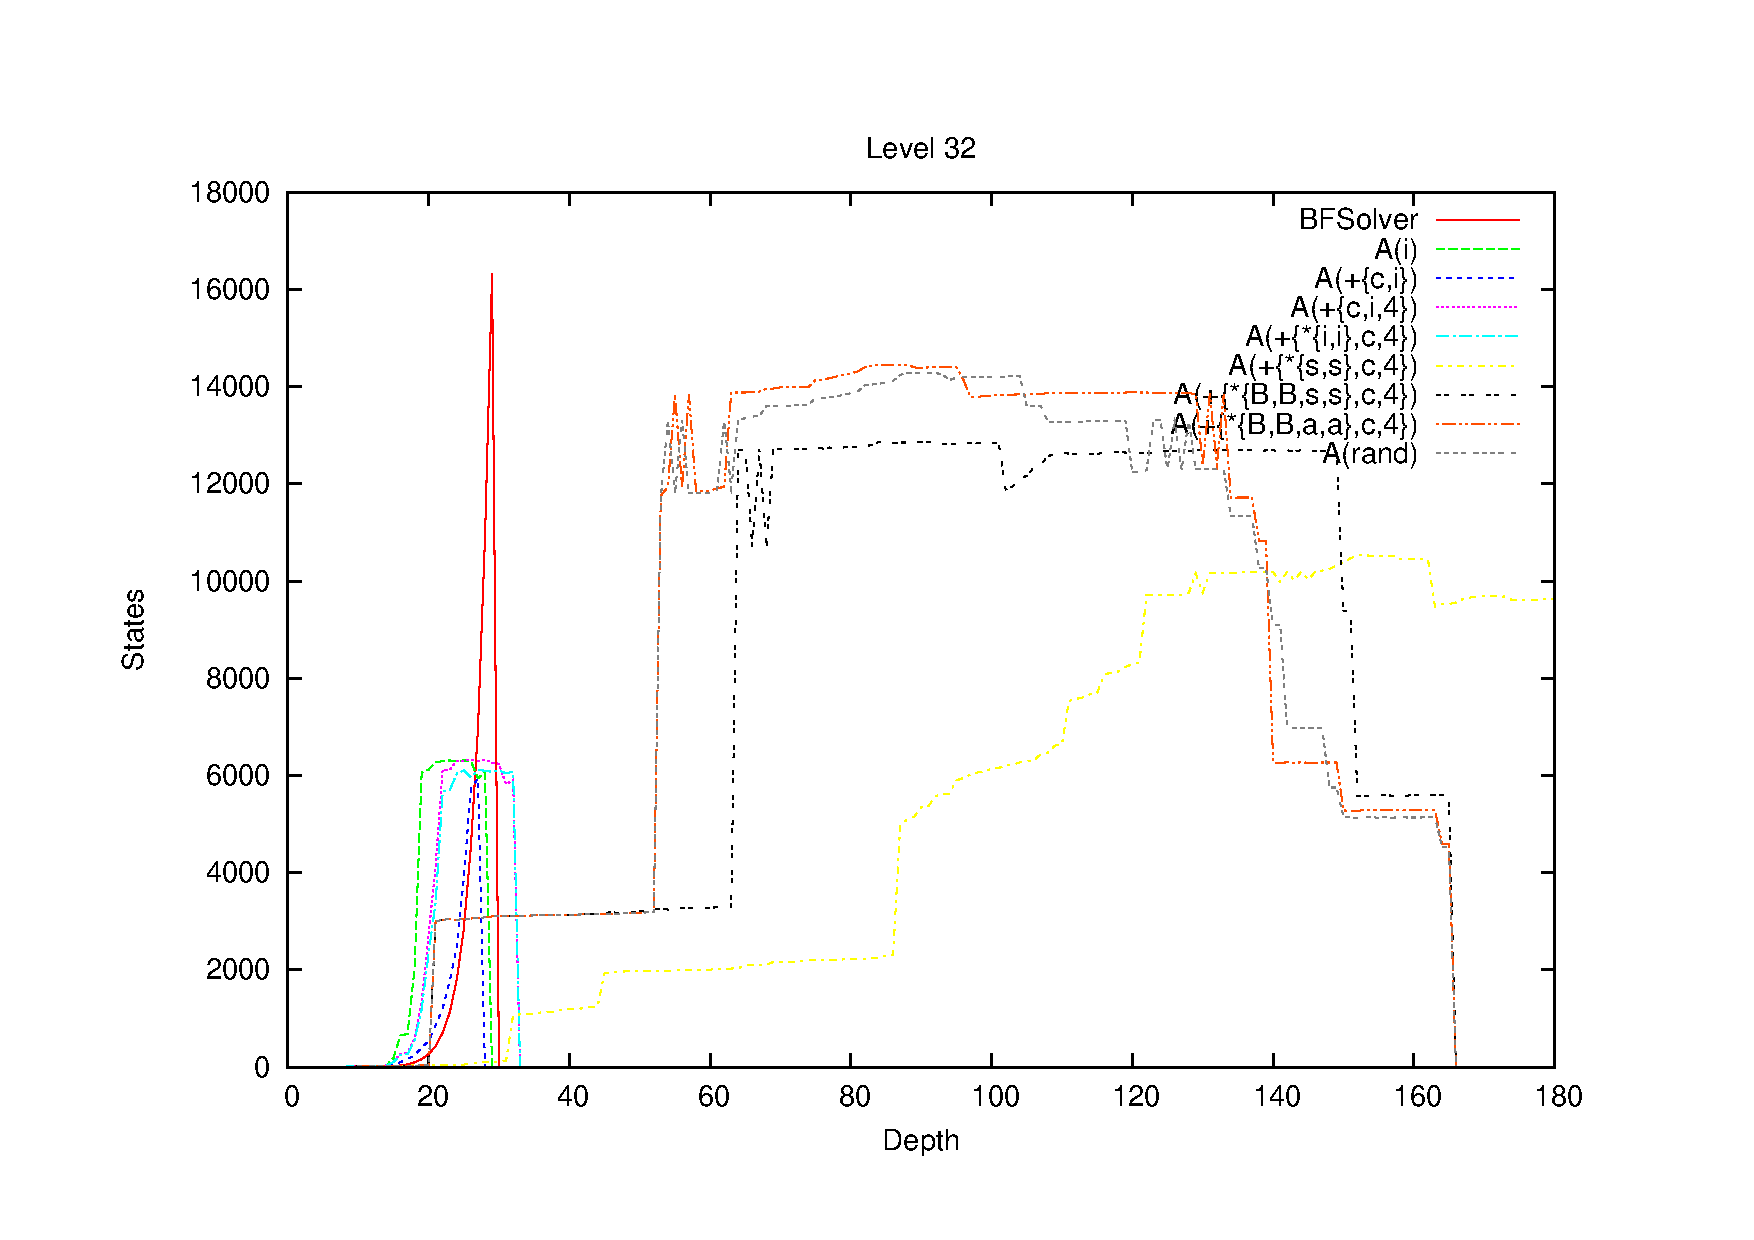
\includegraphics[width=0.85\textwidth]{level32-5}
  \caption{Level 32}
  \label{fig:level32-stats}
\end{figure}

\begin{figure}
  \centering
  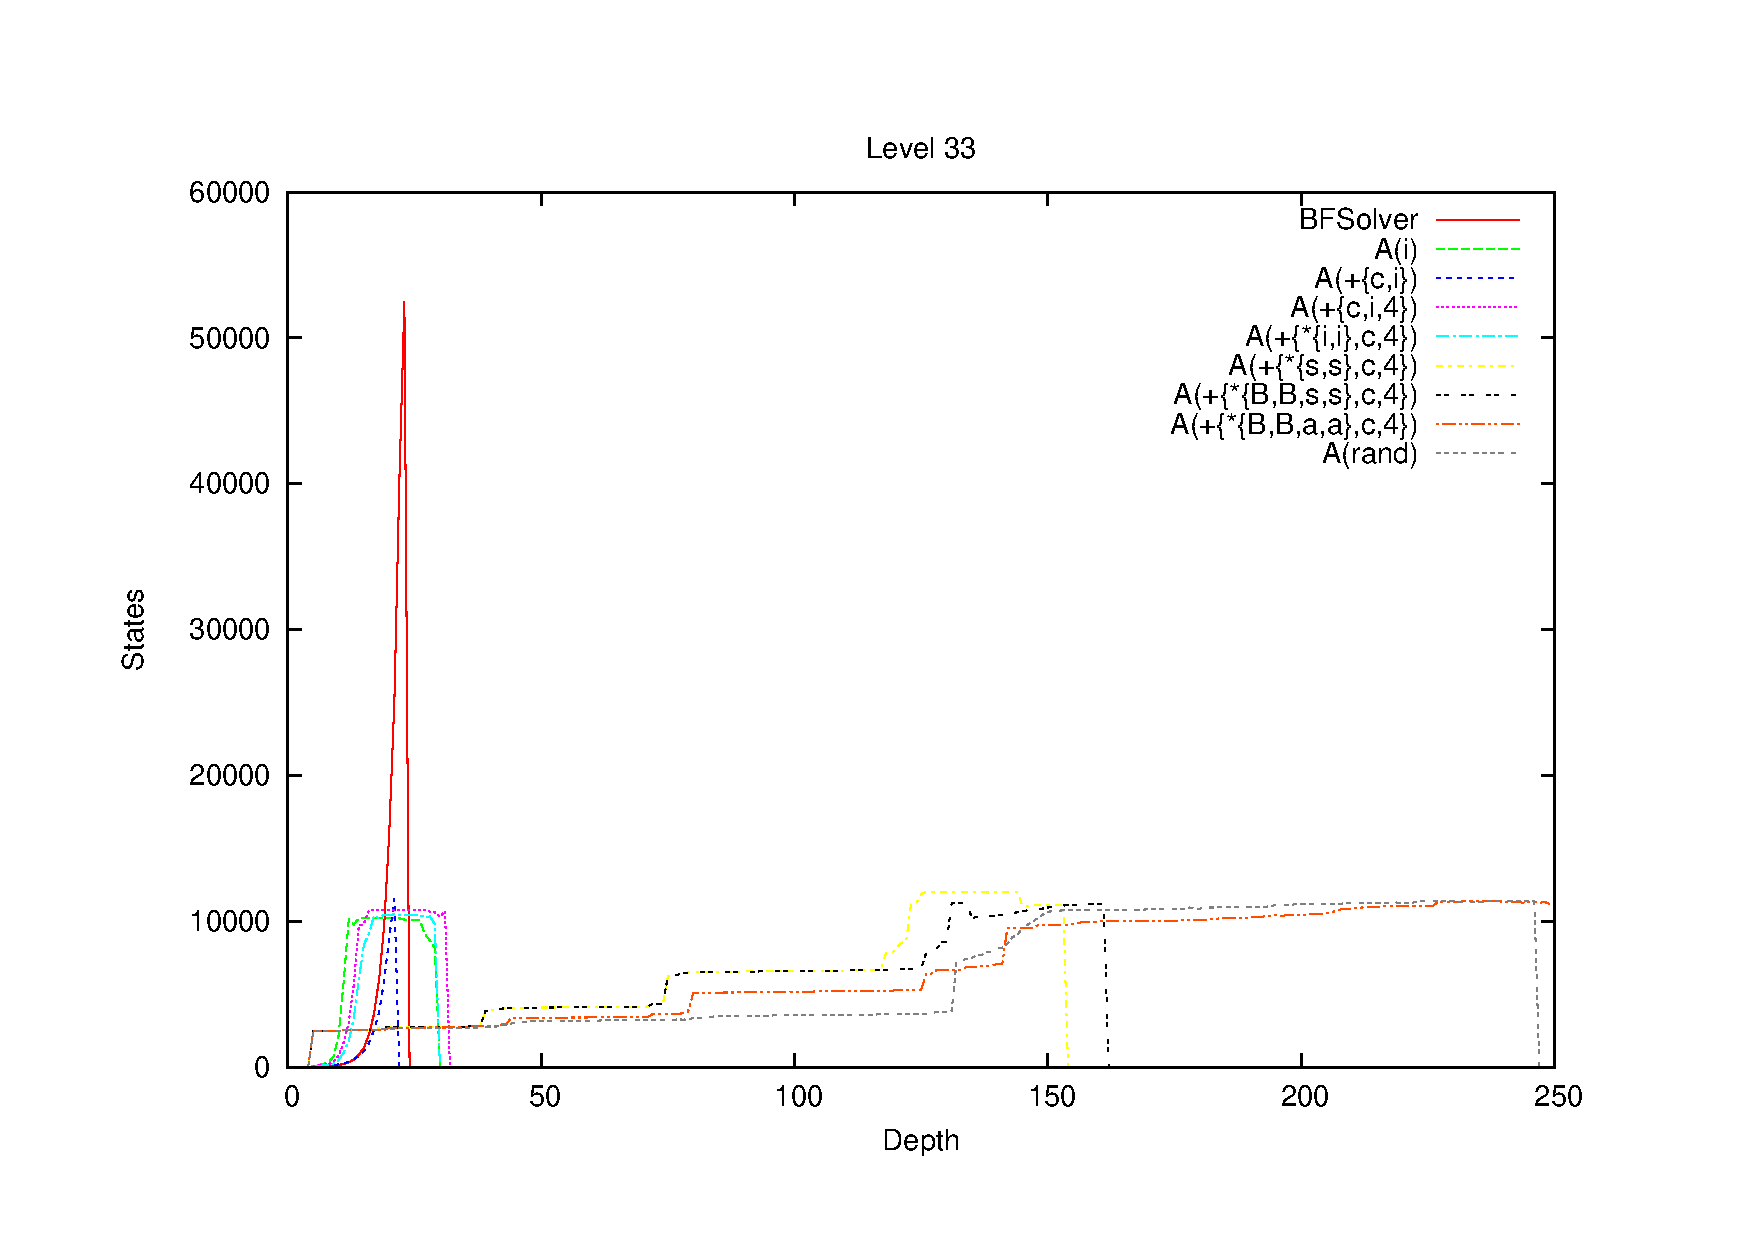
\includegraphics[width=0.85\textwidth]{level33-5}
  \caption{Level 33}
  \label{fig:level33-stats}
\end{figure}
 
\begin{figure}
  \centering
  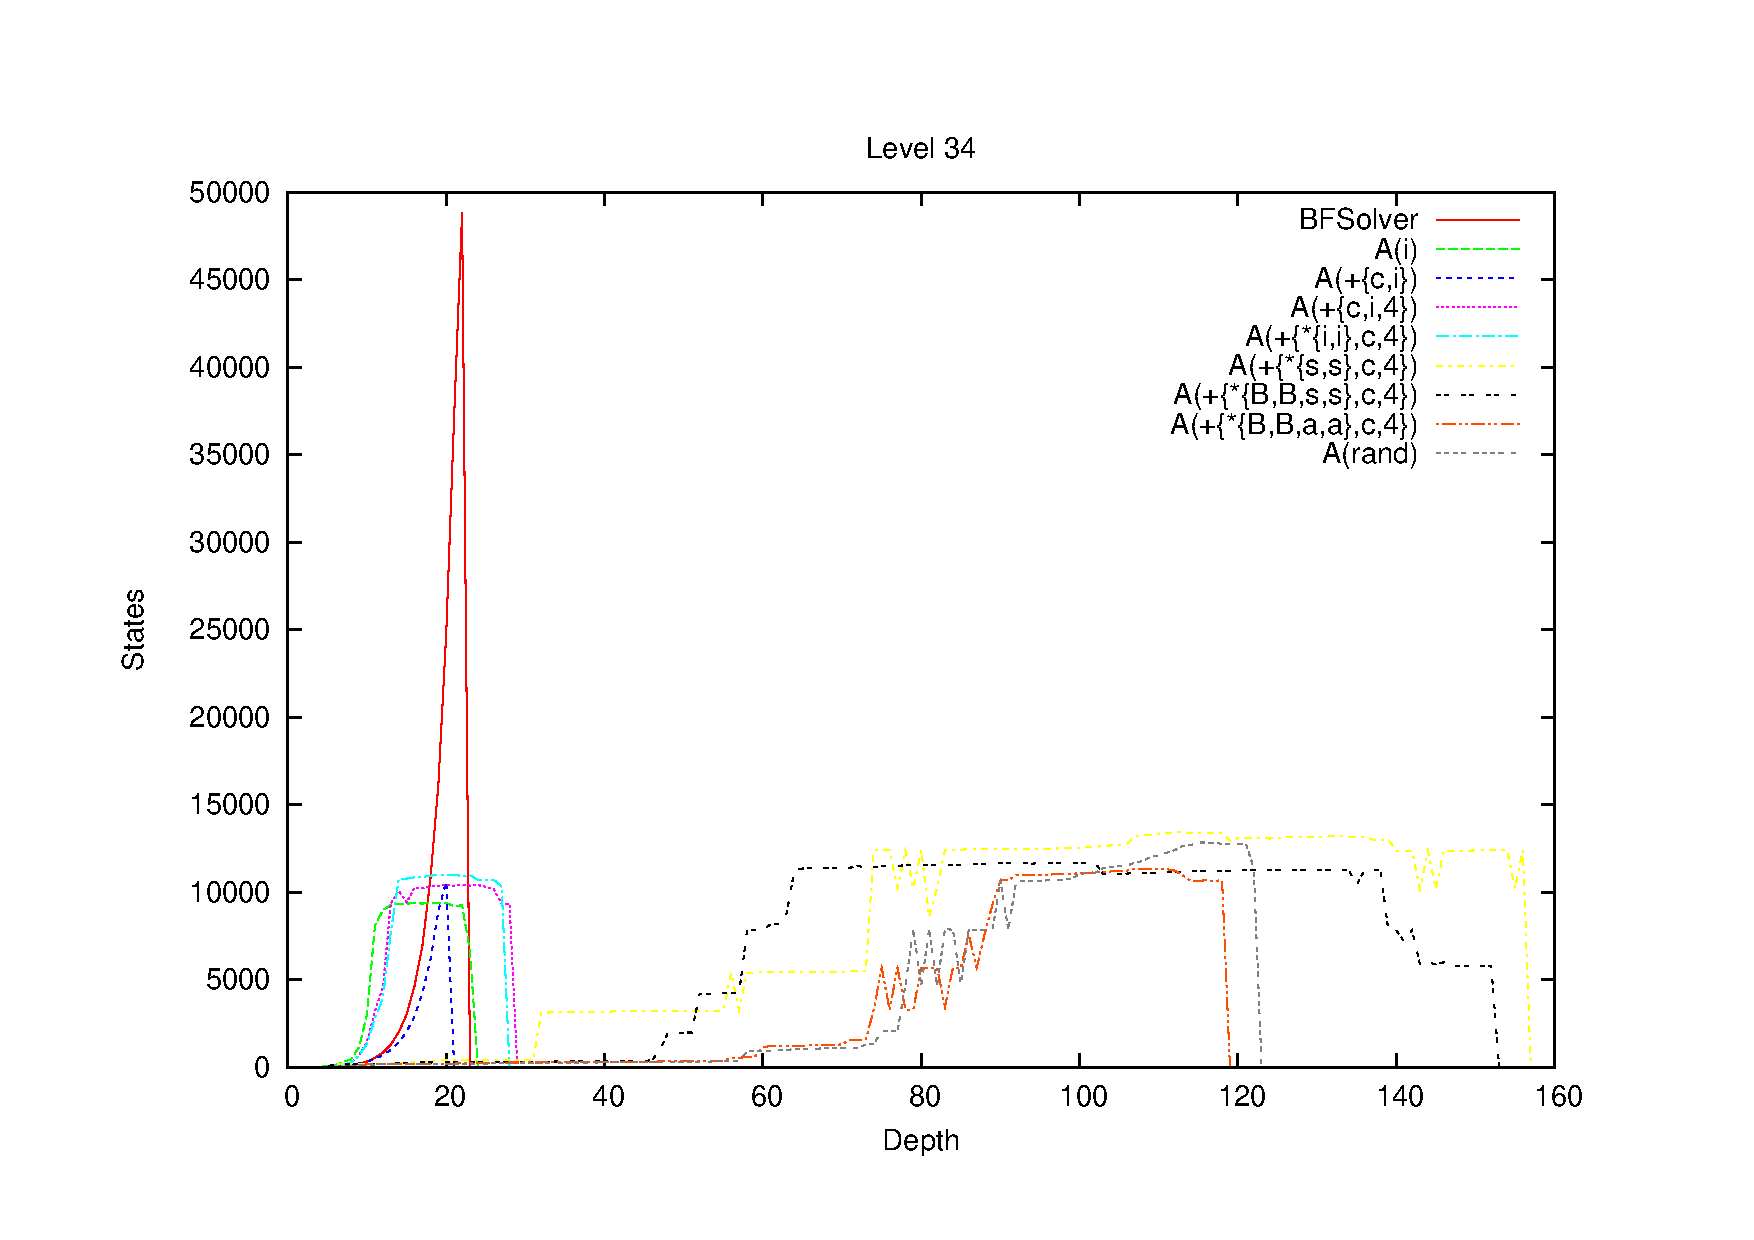
\includegraphics[width=0.85\textwidth]{level34-5}
  \caption{Level 34}
  \label{fig:level34-stats}
\end{figure}

\begin{figure}
  \centering
  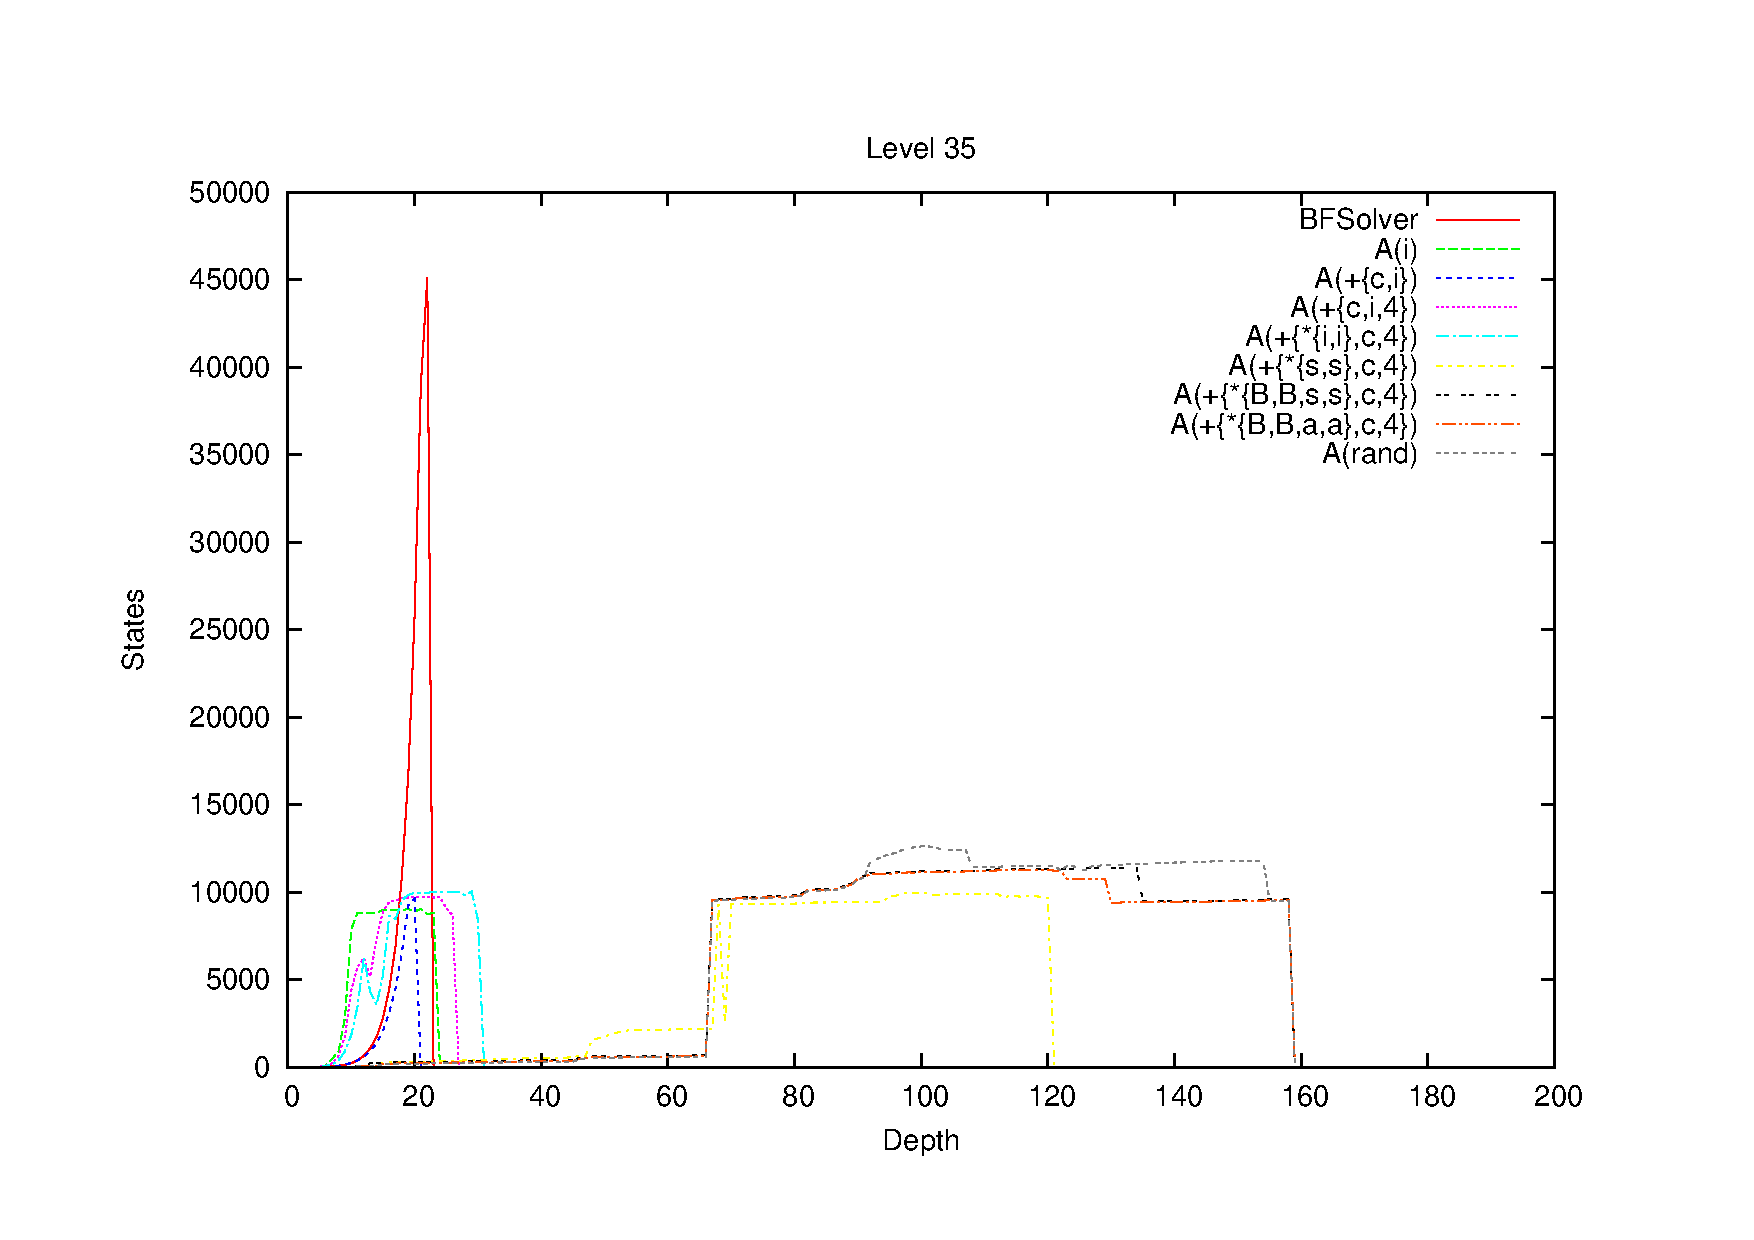
\includegraphics[width=0.85\textwidth]{level35-5}
  \caption{Level 35}
  \label{fig:level35-stats}
\end{figure}
 
\begin{figure}
  \centering
  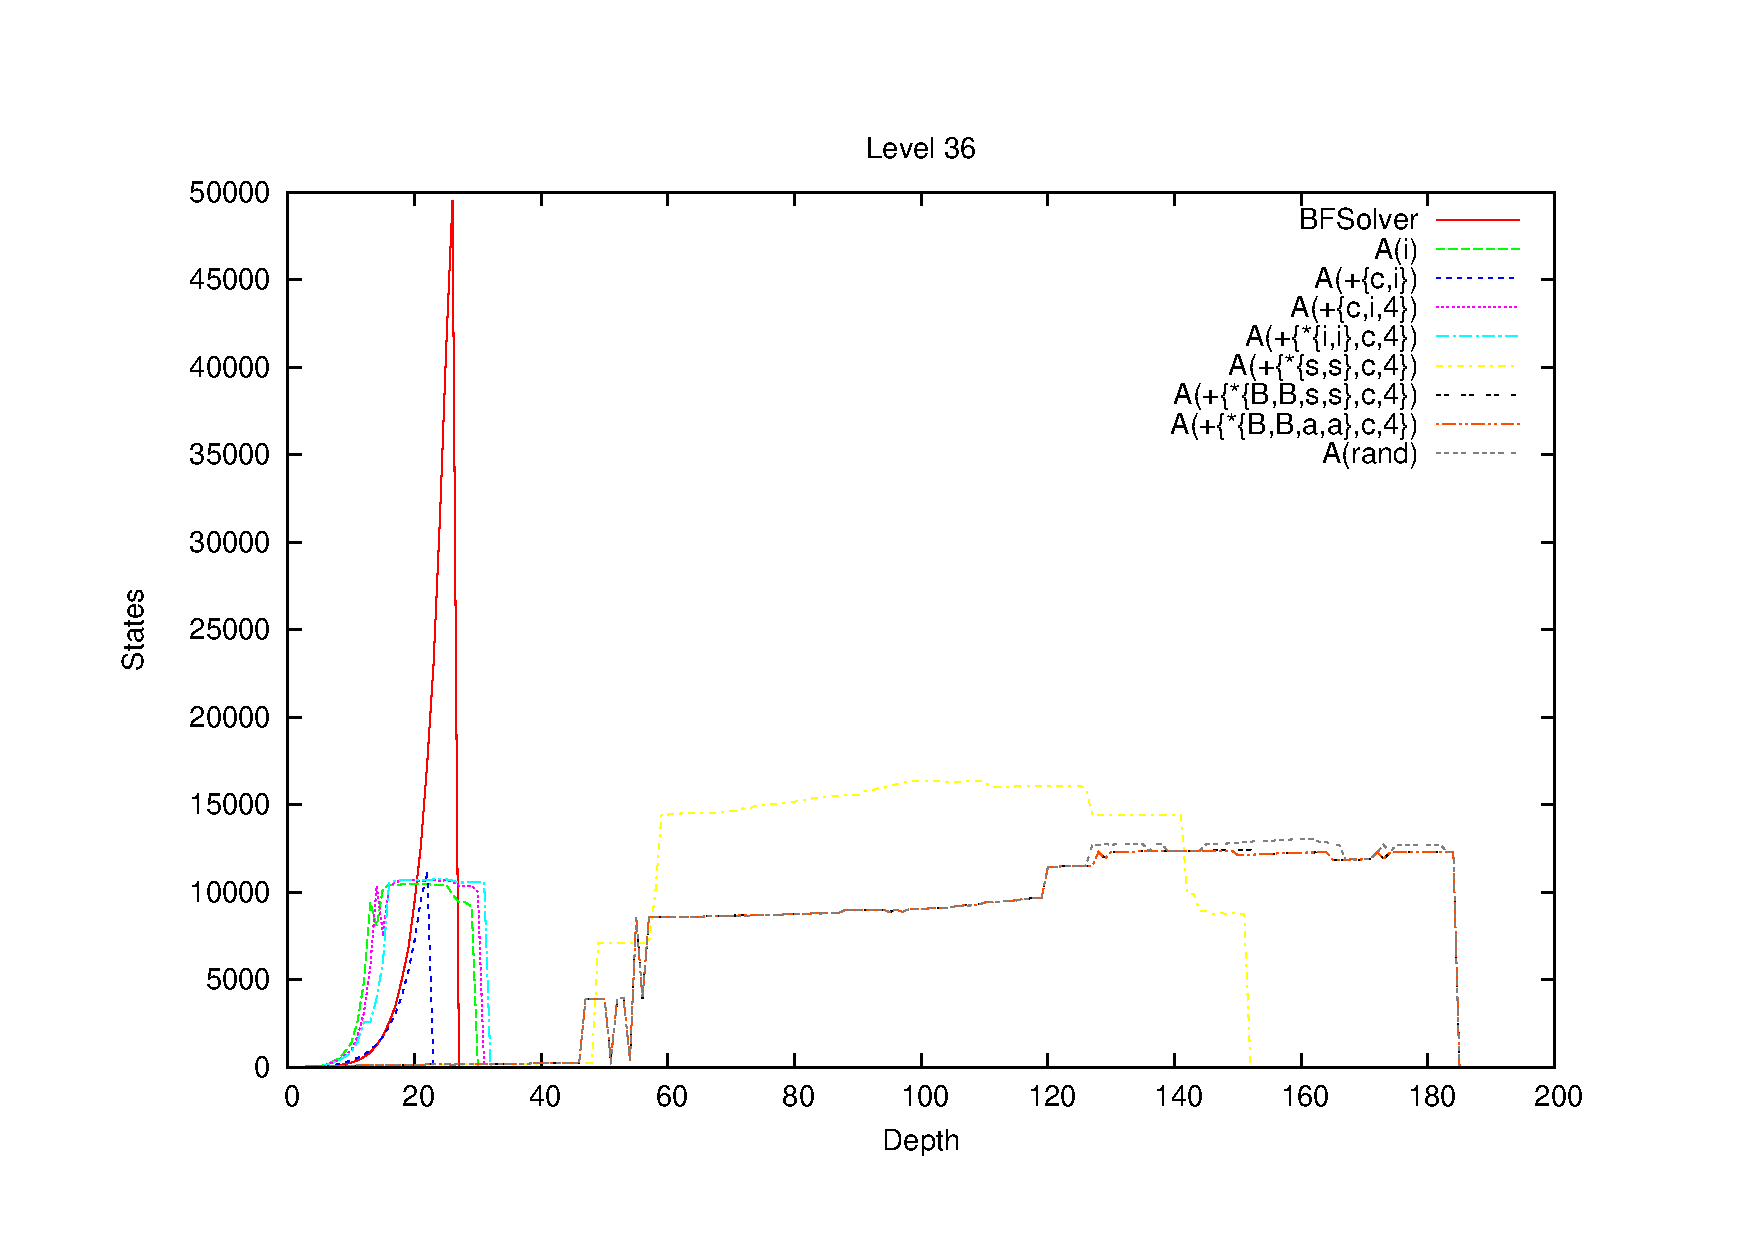
\includegraphics[width=0.85\textwidth]{level36-5}
  \caption{Level 36}
  \label{fig:level36-stats}
\end{figure}

\begin{figure}
  \centering
  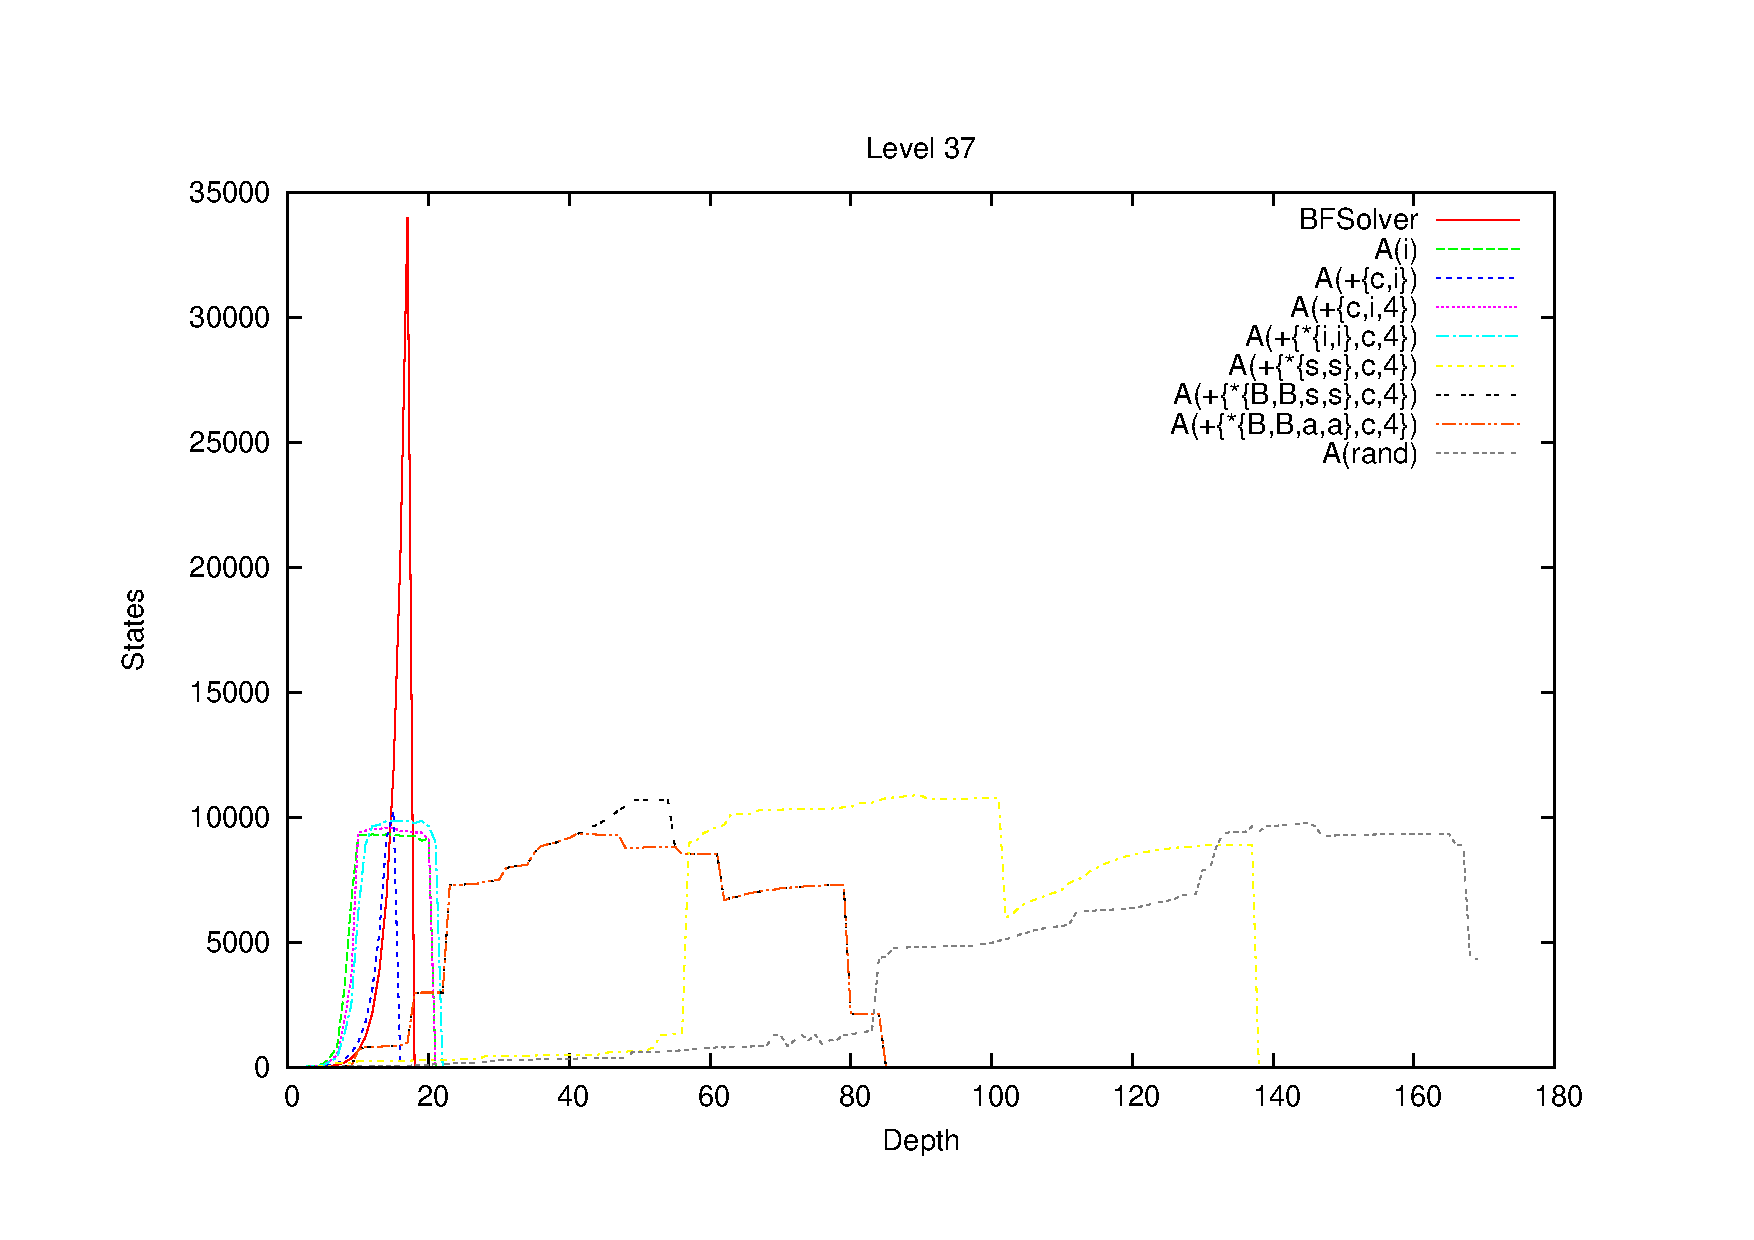
\includegraphics[width=0.85\textwidth]{level37-5}
  \caption{Level 37}
  \label{fig:level37-stats}
\end{figure}
 
\begin{figure}
  \centering
  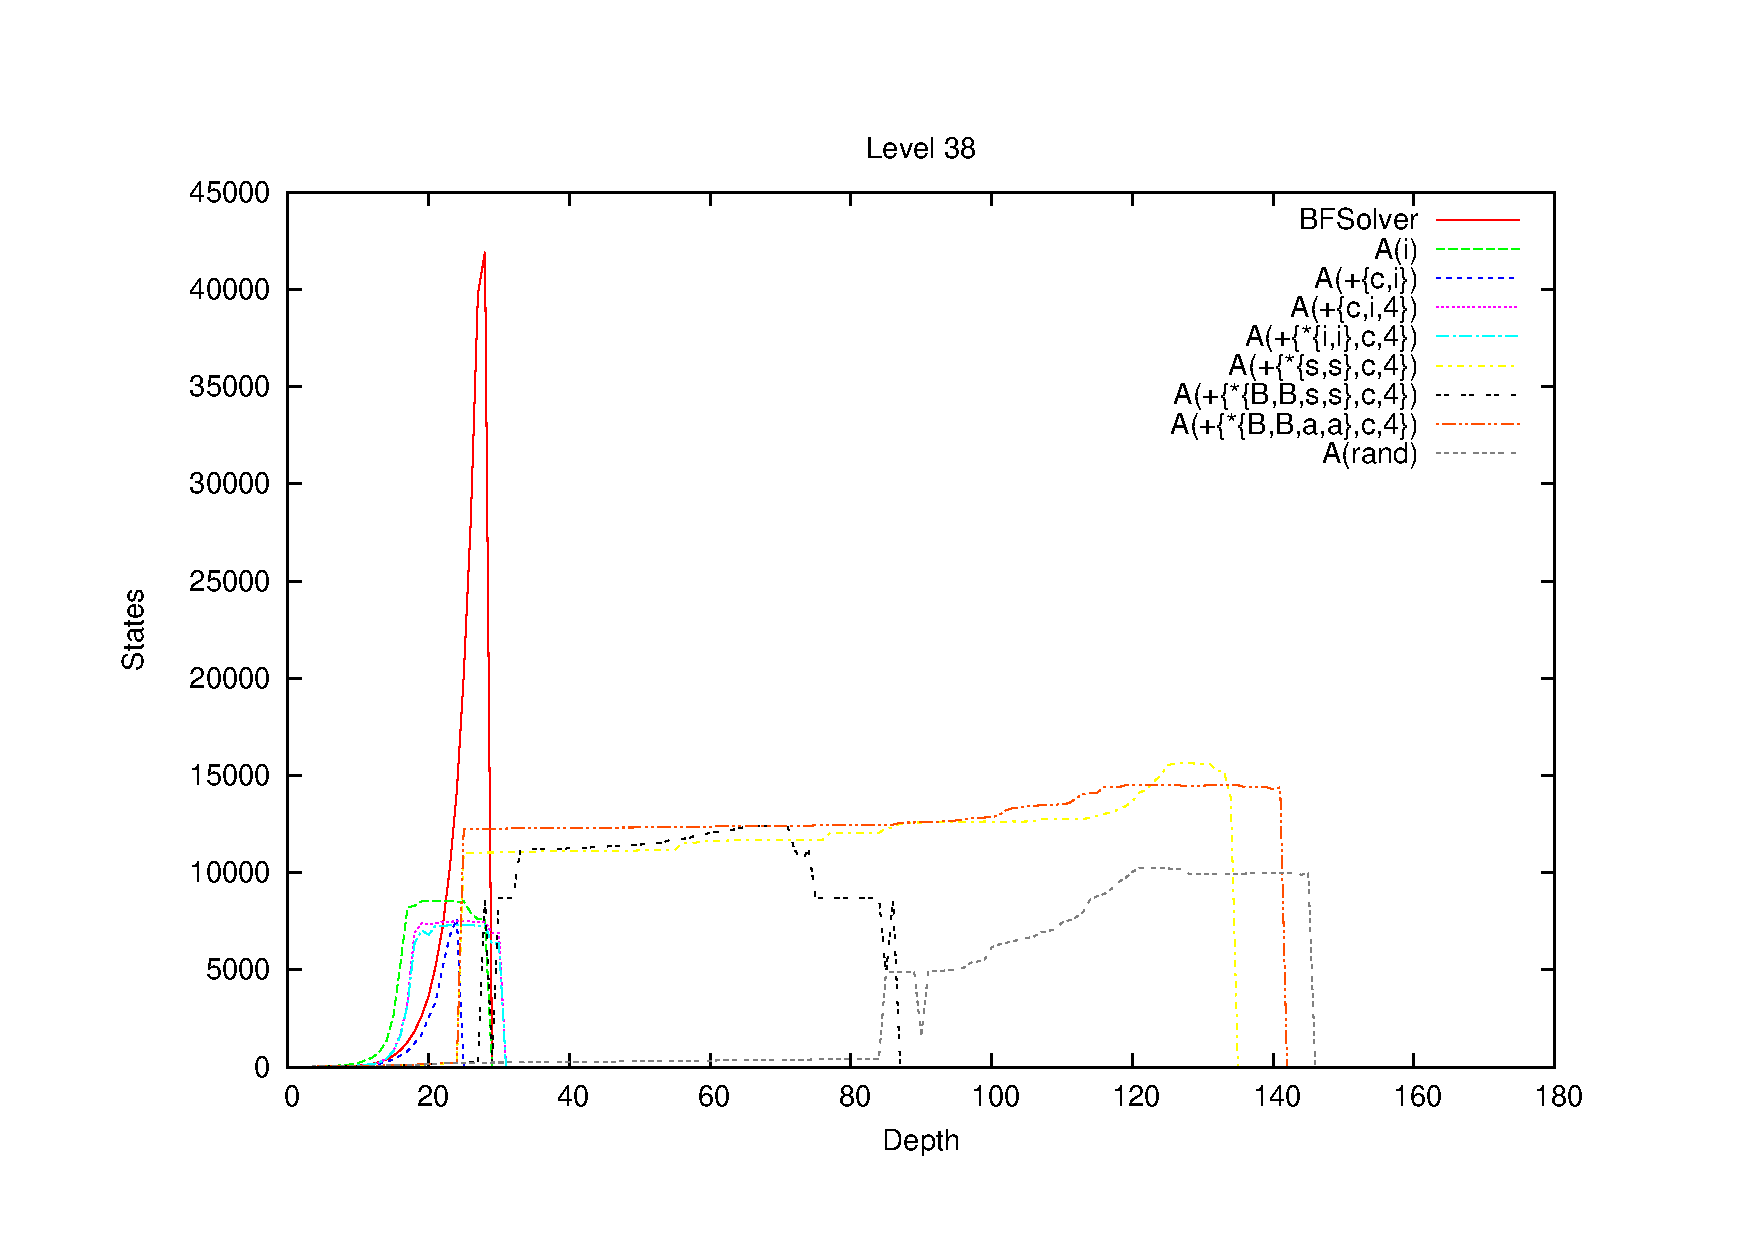
\includegraphics[width=0.85\textwidth]{level38-5}
  \caption{Level 38}
  \label{fig:level38-stats}
\end{figure}

\begin{figure}
  \centering
  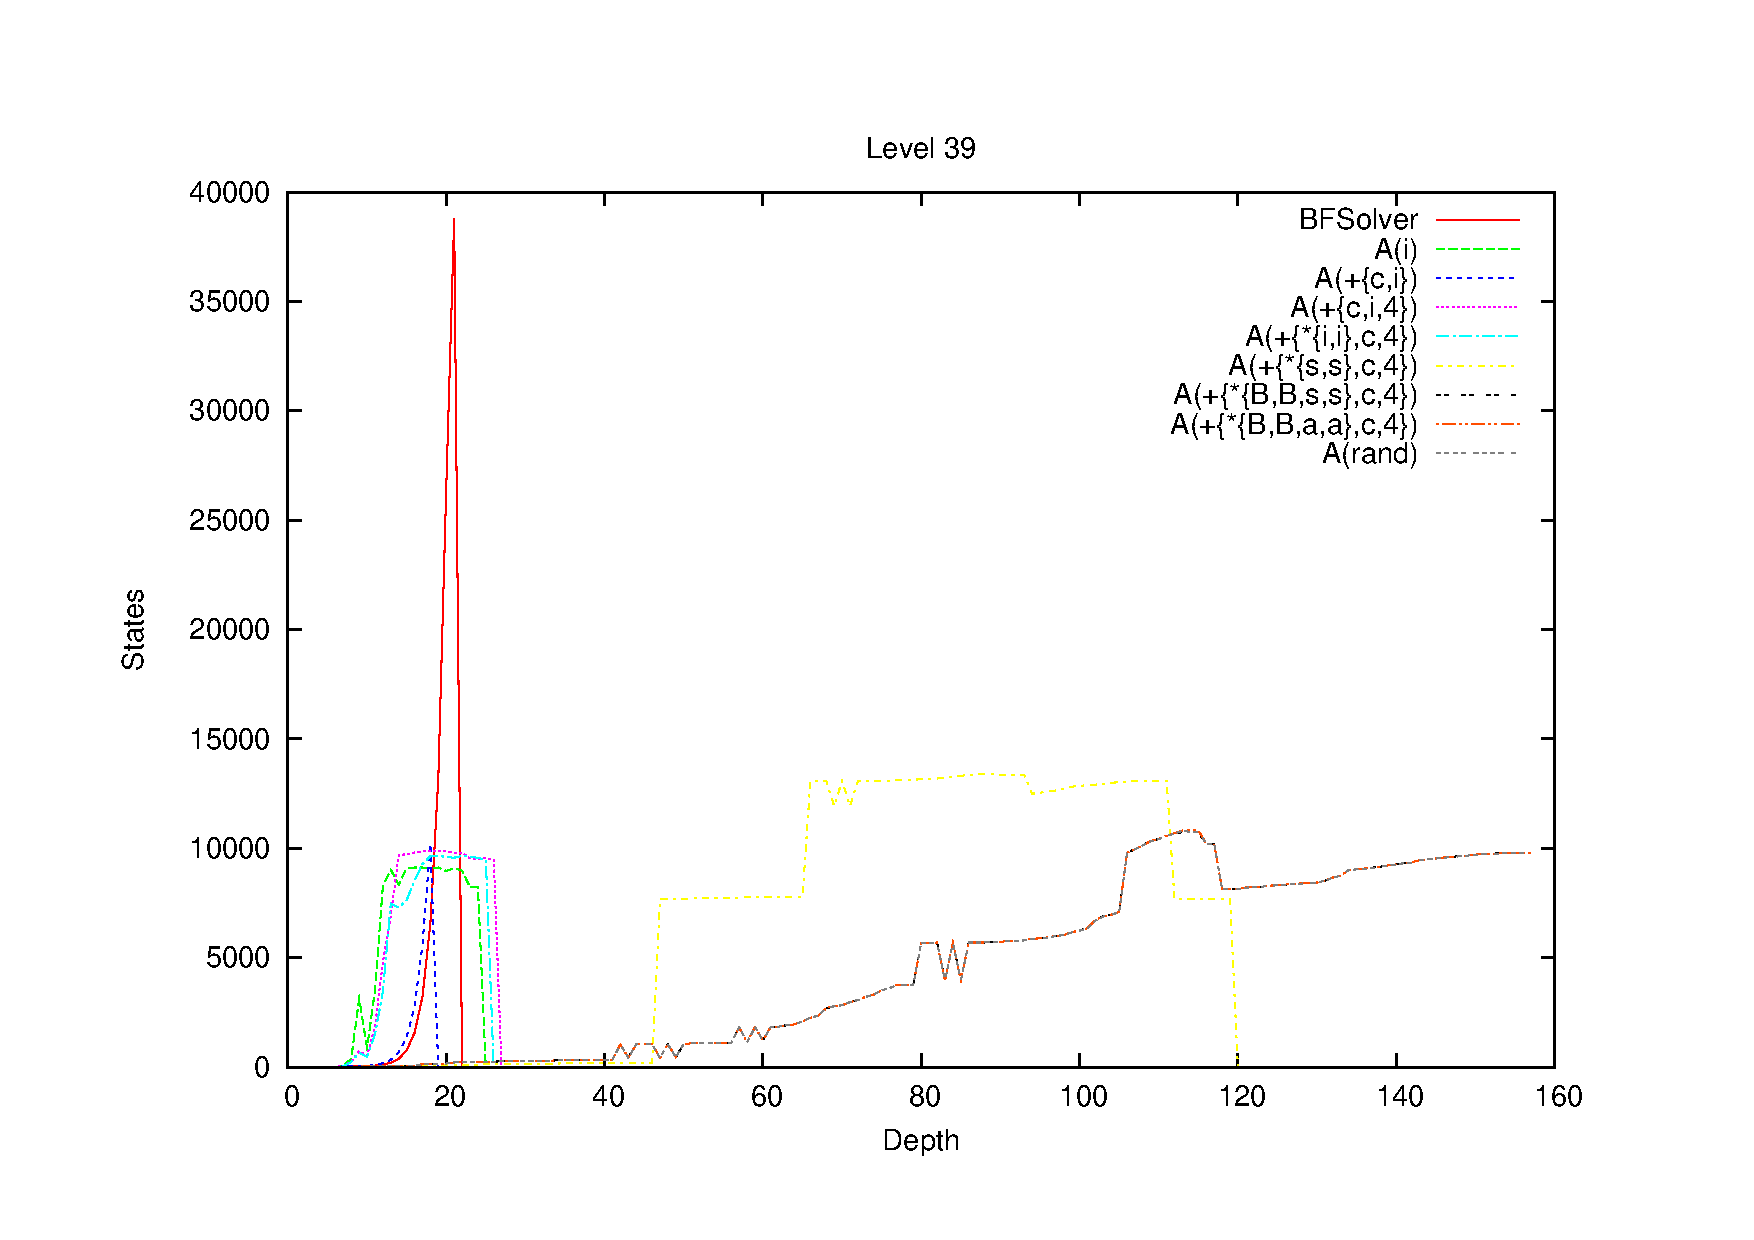
\includegraphics[width=0.85\textwidth]{level39-5}
  \caption{Level 39}
  \label{fig:level39-stats}
\end{figure}
 
\begin{figure}
  \centering
  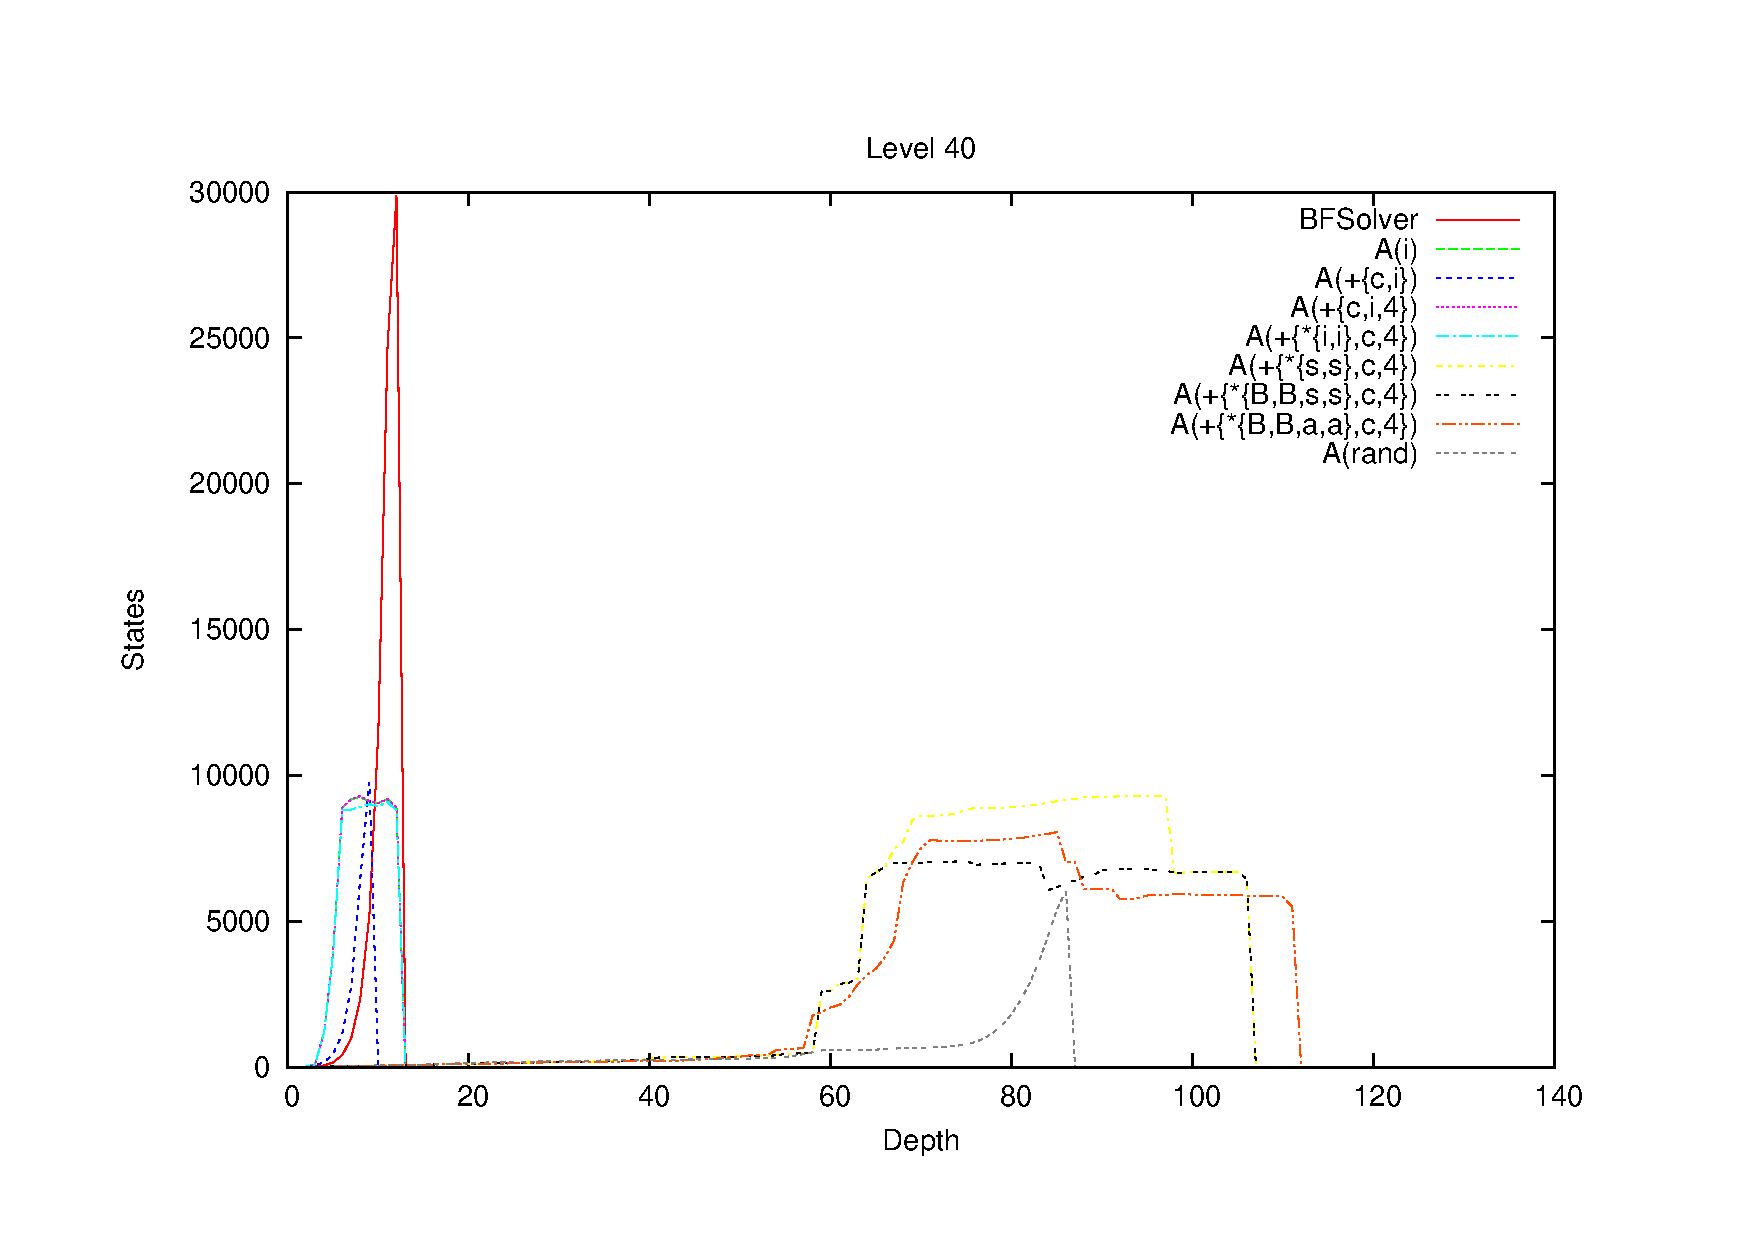
\includegraphics[width=0.85\textwidth]{level40-5}
  \caption{Level 40}
  \label{fig:level40-stats}
\end{figure}

\clearpage

\chapter{Solutions for the Target Level Set}
\label{app:solutions}

Here we present the solution statistics for the target level set
(levelset 0).

For each of the level (represented below with a table) the solver
mentioned under \textbf{Name} was run with a $10$ second timeout.  The
length of the solution trace was noted under \textbf{Steps} (or $0$ if
no solution was found within the alloted time). The time it took to
come to this conclusion is noted in the \textbf{Time} column.

\begin{table}
  \centering
  \begin{tabular}{lrr}
    \toprule
    \textbf{ Name } & \textbf{ Time } & \textbf{ Steps }\\\midrule
    $BFSolver$ & 81 & 33 \\
    $A(+\{*\{i,i\},c,4\})$ & 23 & 36 \\
    $A(+\{*\{s,s\},c,4\})$ & 16 & 36 \\
    $A(+\{*\{B,B,s,s\},c,4\})$ & 13 & 36 \\
    $A(+\{*\{B,B,a,a\},c,4\})$ & 18 & 36 \\
    \bottomrule
  \end{tabular}
  \caption{Level 01}
  \label{tab:level_01}
\end{table}

\begin{table} \centering \begin{tabular}{lrr}\toprule \textbf{ Name }
    & \textbf{ Time } & \textbf{ Steps }\\\midrule
    $BFSolver$ & 58 & 16 \\
    $A(+\{*\{i,i\},c,4\})$ & 6 & 19 \\
    $A(+\{*\{s,s\},c,4\})$ & 6 & 19 \\
    $A(+\{*\{B,B,s,s\},c,4\})$ & 3 & 19 \\
    $A(+\{*\{B,B,a,a\},c,4\})$ & 3 & 19 \\
    \bottomrule \end{tabular} \caption{Level 02}
  \label{tab:level_02} \end{table}

\begin{table} \centering \begin{tabular}{lrr}\toprule \textbf{ Name }
    & \textbf{ Time } & \textbf{ Steps }\\\midrule
    $BFSolver$ & 99 & 41 \\
    $A(+\{*\{i,i\},c,4\})$ & 59 & 44 \\
    $A(+\{*\{s,s\},c,4\})$ & 27 & 42 \\
    $A(+\{*\{B,B,s,s\},c,4\})$ & 27 & 42 \\
    $A(+\{*\{B,B,a,a\},c,4\})$ & 27 & 42 \\
    \bottomrule \end{tabular} \caption{Level 03}
  \label{tab:level_03} \end{table}

\begin{table} \centering \begin{tabular}{lrr}\toprule \textbf{ Name }
    & \textbf{ Time } & \textbf{ Steps }\\\midrule
    $BFSolver$ & 1438 & 23 \\
    $A(+\{*\{i,i\},c,4\})$ & 63 & 32 \\
    $A(+\{*\{s,s\},c,4\})$ & 90 & 32 \\
    $A(+\{*\{B,B,s,s\},c,4\})$ & 23 & 32 \\
    $A(+\{*\{B,B,a,a\},c,4\})$ & 28 & 40 \\
    \bottomrule \end{tabular} \caption{Level 04}
  \label{tab:level_04} \end{table}

\begin{table} \centering \begin{tabular}{lrr}\toprule \textbf{ Name }
    & \textbf{ Time } & \textbf{ Steps }\\\midrule
    $BFSolver$ & 10000 & 0 \\
    $A(+\{*\{i,i\},c,4\})$ & 79 & 32 \\
    $A(+\{*\{s,s\},c,4\})$ & 112 & 32 \\
    $A(+\{*\{B,B,s,s\},c,4\})$ & 15 & 48 \\
    $A(+\{*\{B,B,a,a\},c,4\})$ & 17 & 42 \\
    \bottomrule \end{tabular} \caption{Level 05}
  \label{tab:level_05} \end{table}

\begin{table} \centering \begin{tabular}{lrr}\toprule \textbf{ Name }
    & \textbf{ Time } & \textbf{ Steps }\\\midrule
    $BFSolver$ & 4138 & 107 \\
    $A(+\{*\{i,i\},c,4\})$ & 1208 & 118 \\
    $A(+\{*\{s,s\},c,4\})$ & 797 & 146 \\
    $A(+\{*\{B,B,s,s\},c,4\})$ & 339 & 146 \\
    $A(+\{*\{B,B,a,a\},c,4\})$ & 266 & 150 \\
    \bottomrule \end{tabular} \caption{Level 06}
  \label{tab:level_06} \end{table}

\begin{table} \centering \begin{tabular}{lrr}\toprule \textbf{ Name }
    & \textbf{ Time } & \textbf{ Steps }\\\midrule
    $BFSolver$ & 10201 & 0 \\
    $A(+\{*\{i,i\},c,4\})$ & 62 & 33 \\
    $A(+\{*\{s,s\},c,4\})$ & 12 & 33 \\
    $A(+\{*\{B,B,s,s\},c,4\})$ & 59 & 61 \\
    $A(+\{*\{B,B,a,a\},c,4\})$ & 60 & 61 \\
    \bottomrule \end{tabular} \caption{Level 07a}
  \label{tab:level_07a} \end{table}

\begin{table} \centering \begin{tabular}{lrr}\toprule \textbf{ Name }
    & \textbf{ Time } & \textbf{ Steps }\\\midrule
    $BFSolver$ & 10344 & 0 \\
    $A(+\{*\{i,i\},c,4\})$ & 61 & 32 \\
    $A(+\{*\{s,s\},c,4\})$ & 30 & 32 \\
    $A(+\{*\{B,B,s,s\},c,4\})$ & 7 & 34 \\
    $A(+\{*\{B,B,a,a\},c,4\})$ & 8 & 34 \\
    \bottomrule \end{tabular} \caption{Level 07b}
  \label{tab:level_07b} \end{table}

\begin{table} \centering \begin{tabular}{lrr}\toprule \textbf{ Name }
    & \textbf{ Time } & \textbf{ Steps }\\\midrule
    $BFSolver$ & 10279 & 0 \\
    $A(+\{*\{i,i\},c,4\})$ & 623 & 37 \\
    $A(+\{*\{s,s\},c,4\})$ & 860 & 37 \\
    $A(+\{*\{B,B,s,s\},c,4\})$ & 139 & 57 \\
    $A(+\{*\{B,B,a,a\},c,4\})$ & 43 & 57 \\
    \bottomrule \end{tabular} \caption{Level 07}
  \label{tab:level_07} \end{table}

\begin{table} \centering \begin{tabular}{lrr}\toprule \textbf{ Name }
    & \textbf{ Time } & \textbf{ Steps }\\\midrule
    $BFSolver$ & 258 & 97 \\
    $A(+\{*\{i,i\},c,4\})$ & 87 & 112 \\
    $A(+\{*\{s,s\},c,4\})$ & 89 & 112 \\
    $A(+\{*\{B,B,s,s\},c,4\})$ & 85 & 112 \\
    $A(+\{*\{B,B,a,a\},c,4\})$ & 104 & 112 \\
    \bottomrule \end{tabular} \caption{Level 08}
  \label{tab:level_08} \end{table}

\begin{table} \centering \begin{tabular}{lrr}\toprule \textbf{ Name }
    & \textbf{ Time } & \textbf{ Steps }\\\midrule
    $BFSolver$ & 32 & 30 \\
    $A(+\{*\{i,i\},c,4\})$ & 5 & 33 \\
    $A(+\{*\{s,s\},c,4\})$ & 5 & 33 \\
    $A(+\{*\{B,B,s,s\},c,4\})$ & 21 & 33 \\
    $A(+\{*\{B,B,a,a\},c,4\})$ & 4 & 33 \\
    \bottomrule \end{tabular} \caption{Level 09}
  \label{tab:level_09} \end{table}

\begin{table} \centering \begin{tabular}{lrr}\toprule \textbf{ Name }
    & \textbf{ Time } & \textbf{ Steps }\\\midrule
    $BFSolver$ & 327 & 89 \\
    $A(+\{*\{i,i\},c,4\})$ & 79 & 122 \\
    $A(+\{*\{s,s\},c,4\})$ & 83 & 122 \\
    $A(+\{*\{B,B,s,s\},c,4\})$ & 85 & 122 \\
    $A(+\{*\{B,B,a,a\},c,4\})$ & 73 & 112 \\
    \bottomrule \end{tabular} \caption{Level 10}
  \label{tab:level_10} \end{table}

\begin{table} \centering \begin{tabular}{lrr}\toprule \textbf{ Name }
    & \textbf{ Time } & \textbf{ Steps }\\\midrule
    $BFSolver$ & 444 & 78 \\
    $A(+\{*\{i,i\},c,4\})$ & 69 & 87 \\
    $A(+\{*\{s,s\},c,4\})$ & 54 & 83 \\
    $A(+\{*\{B,B,s,s\},c,4\})$ & 44 & 83 \\
    $A(+\{*\{B,B,a,a\},c,4\})$ & 42 & 83 \\
    \bottomrule \end{tabular} \caption{Level 11}
  \label{tab:level_11} \end{table}

\begin{table} \centering \begin{tabular}{lrr}\toprule \textbf{ Name }
    & \textbf{ Time } & \textbf{ Steps }\\\midrule
    $BFSolver$ & 132 & 49 \\
    $A(+\{*\{i,i\},c,4\})$ & 8 & 50 \\
    $A(+\{*\{s,s\},c,4\})$ & 12 & 50 \\
    $A(+\{*\{B,B,s,s\},c,4\})$ & 7 & 50 \\
    $A(+\{*\{B,B,a,a\},c,4\})$ & 7 & 50 \\
    \bottomrule \end{tabular} \caption{Level 12}
  \label{tab:level_12} \end{table}

\begin{table} \centering \begin{tabular}{lrr}\toprule \textbf{ Name }
    & \textbf{ Time } & \textbf{ Steps }\\\midrule
    $BFSolver$ & 1740 & 52 \\
    $A(+\{*\{i,i\},c,4\})$ & 206 & 84 \\
    $A(+\{*\{s,s\},c,4\})$ & 261 & 84 \\
    $A(+\{*\{B,B,s,s\},c,4\})$ & 188 & 84 \\
    $A(+\{*\{B,B,a,a\},c,4\})$ & 158 & 82 \\
    \bottomrule \end{tabular} \caption{Level 13}
  \label{tab:level_13} \end{table}

\begin{table} \centering \begin{tabular}{lrr}\toprule \textbf{ Name }
    & \textbf{ Time } & \textbf{ Steps }\\\midrule
    $BFSolver$ & 61 & 51 \\
    $A(+\{*\{i,i\},c,4\})$ & 9 & 52 \\
    $A(+\{*\{s,s\},c,4\})$ & 9 & 52 \\
    $A(+\{*\{B,B,s,s\},c,4\})$ & 10 & 52 \\
    $A(+\{*\{B,B,a,a\},c,4\})$ & 7 & 52 \\
    \bottomrule \end{tabular} \caption{Level 14}
  \label{tab:level_14} \end{table}

\begin{table} \centering \begin{tabular}{lrr}\toprule \textbf{ Name }
    & \textbf{ Time } & \textbf{ Steps }\\\midrule
    $BFSolver$ & 57 & 37 \\
    $A(+\{*\{i,i\},c,4\})$ & 13 & 38 \\
    $A(+\{*\{s,s\},c,4\})$ & 12 & 38 \\
    $A(+\{*\{B,B,s,s\},c,4\})$ & 12 & 38 \\
    $A(+\{*\{B,B,a,a\},c,4\})$ & 12 & 38 \\
    \bottomrule \end{tabular} \caption{Level 15}
  \label{tab:level_15} \end{table}

\clearpage

\begin{table} \centering \begin{tabular}{lrr}\toprule \textbf{ Name }
    & \textbf{ Time } & \textbf{ Steps }\\\midrule
    $BFSolver$ & 10000 & 0 \\
    $A(+\{*\{i,i\},c,4\})$ & 796 & 129 \\
    $A(+\{*\{s,s\},c,4\})$ & 98 & 123 \\
    $A(+\{*\{B,B,s,s\},c,4\})$ & 667 & 123 \\
    $A(+\{*\{B,B,a,a\},c,4\})$ & 624 & 123 \\
    \bottomrule \end{tabular} \caption{Level 16}
  \label{tab:level_16} \end{table}

\begin{table} \centering \begin{tabular}{lrr}\toprule \textbf{ Name }
    & \textbf{ Time } & \textbf{ Steps }\\\midrule
    $BFSolver$ & 279 & 25 \\
    $A(+\{*\{i,i\},c,4\})$ & 6 & 27 \\
    $A(+\{*\{s,s\},c,4\})$ & 8 & 27 \\
    $A(+\{*\{B,B,s,s\},c,4\})$ & 8 & 27 \\
    $A(+\{*\{B,B,a,a\},c,4\})$ & 7 & 27 \\
    \bottomrule \end{tabular} \caption{Level 17}
  \label{tab:level_17} \end{table}

\begin{table} \centering \begin{tabular}{lrr}\toprule \textbf{ Name }
    & \textbf{ Time } & \textbf{ Steps }\\\midrule
    $BFSolver$ & 269 & 71 \\
    $A(+\{*\{i,i\},c,4\})$ & 37 & 78 \\
    $A(+\{*\{s,s\},c,4\})$ & 33 & 78 \\
    $A(+\{*\{B,B,s,s\},c,4\})$ & 44 & 100 \\
    $A(+\{*\{B,B,a,a\},c,4\})$ & 41 & 100 \\
    \bottomrule \end{tabular} \caption{Level 18}
  \label{tab:level_18} \end{table}

\begin{table} \centering \begin{tabular}{lrr}\toprule \textbf{ Name }
    & \textbf{ Time } & \textbf{ Steps }\\\midrule
    $BFSolver$ & 77 & 41 \\
    $A(+\{*\{i,i\},c,4\})$ & 44 & 51 \\
    $A(+\{*\{s,s\},c,4\})$ & 44 & 51 \\
    $A(+\{*\{B,B,s,s\},c,4\})$ & 27 & 51 \\
    $A(+\{*\{B,B,a,a\},c,4\})$ & 25 & 51 \\
    \bottomrule \end{tabular} \caption{Level 19}
  \label{tab:level_19} \end{table}

\begin{table} \centering \begin{tabular}{lrr}\toprule \textbf{ Name }
    & \textbf{ Time } & \textbf{ Steps }\\\midrule
    $BFSolver$ & 199 & 50 \\
    $A(+\{*\{i,i\},c,4\})$ & 74 & 67 \\
    $A(+\{*\{s,s\},c,4\})$ & 69 & 67 \\
    $A(+\{*\{B,B,s,s\},c,4\})$ & 60 & 67 \\
    $A(+\{*\{B,B,a,a\},c,4\})$ & 59 & 67 \\
    \bottomrule \end{tabular} \caption{Level 20}
  \label{tab:level_20} \end{table}

\begin{table} \centering \begin{tabular}{lrr}\toprule \textbf{ Name }
    & \textbf{ Time } & \textbf{ Steps }\\\midrule
    $BFSolver$ & 41 & 17 \\
    $A(+\{*\{i,i\},c,4\})$ & 2 & 18 \\
    $A(+\{*\{s,s\},c,4\})$ & 2 & 18 \\
    $A(+\{*\{B,B,s,s\},c,4\})$ & 4 & 20 \\
    $A(+\{*\{B,B,a,a\},c,4\})$ & 5 & 20 \\
    \bottomrule \end{tabular} \caption{Level 21}
  \label{tab:level_21} \end{table}

\begin{table} \centering \begin{tabular}{lrr}\toprule \textbf{ Name }
    & \textbf{ Time } & \textbf{ Steps }\\\midrule
    $BFSolver$ & 548 & 47 \\
    $A(+\{*\{i,i\},c,4\})$ & 147 & 68 \\
    $A(+\{*\{s,s\},c,4\})$ & 102 & 66 \\
    $A(+\{*\{B,B,s,s\},c,4\})$ & 152 & 66 \\
    $A(+\{*\{B,B,a,a\},c,4\})$ & 149 & 66 \\
    \bottomrule \end{tabular} \caption{Level 22}
  \label{tab:level_22} \end{table}

\begin{table} \centering \begin{tabular}{lrr}\toprule \textbf{ Name }
    & \textbf{ Time } & \textbf{ Steps }\\\midrule
    $BFSolver$ & 53 & 56 \\
    $A(+\{*\{i,i\},c,4\})$ & 17 & 59 \\
    $A(+\{*\{s,s\},c,4\})$ & 17 & 59 \\
    $A(+\{*\{B,B,s,s\},c,4\})$ & 14 & 59 \\
    $A(+\{*\{B,B,a,a\},c,4\})$ & 14 & 59 \\
    \bottomrule \end{tabular} \caption{Level 23}
  \label{tab:level_23} \end{table}

\begin{table} \centering \begin{tabular}{lrr}\toprule \textbf{ Name }
    & \textbf{ Time } & \textbf{ Steps }\\\midrule
    $BFSolver$ & 118 & 35 \\
    $A(+\{*\{i,i\},c,4\})$ & 17 & 48 \\
    $A(+\{*\{s,s\},c,4\})$ & 16 & 48 \\
    $A(+\{*\{B,B,s,s\},c,4\})$ & 17 & 48 \\
    $A(+\{*\{B,B,a,a\},c,4\})$ & 18 & 48 \\
    \bottomrule \end{tabular} \caption{Level 24}
  \label{tab:level_24} \end{table}

\begin{table} \centering \begin{tabular}{lrr}\toprule \textbf{ Name }
    & \textbf{ Time } & \textbf{ Steps }\\\midrule
    $BFSolver$ & 641 & 29 \\
    $A(+\{*\{i,i\},c,4\})$ & 16 & 30 \\
    $A(+\{*\{s,s\},c,4\})$ & 18 & 30 \\
    $A(+\{*\{B,B,s,s\},c,4\})$ & 18 & 34 \\
    $A(+\{*\{B,B,a,a\},c,4\})$ & 6 & 30 \\
    \bottomrule \end{tabular} \caption{Level 25}
  \label{tab:level_25} \end{table}

\begin{table} \centering \begin{tabular}{lrr}\toprule \textbf{ Name }
    & \textbf{ Time } & \textbf{ Steps }\\\midrule
    $BFSolver$ & 631 & 41 \\
    $A(+\{*\{i,i\},c,4\})$ & 33 & 42 \\
    $A(+\{*\{s,s\},c,4\})$ & 38 & 42 \\
    $A(+\{*\{B,B,s,s\},c,4\})$ & 79 & 42 \\
    $A(+\{*\{B,B,a,a\},c,4\})$ & 27 & 42 \\
    \bottomrule \end{tabular} \caption{Level 26}
  \label{tab:level_26} \end{table}

\begin{table} \centering \begin{tabular}{lrr}\toprule \textbf{ Name }
    & \textbf{ Time } & \textbf{ Steps }\\\midrule
    $BFSolver$ & 72 & 50 \\
    $A(+\{*\{i,i\},c,4\})$ & 35 & 51 \\
    $A(+\{*\{s,s\},c,4\})$ & 20 & 51 \\
    $A(+\{*\{B,B,s,s\},c,4\})$ & 18 & 51 \\
    $A(+\{*\{B,B,a,a\},c,4\})$ & 14 & 51 \\
    \bottomrule \end{tabular} \caption{Level 27}
  \label{tab:level_27} \end{table}

\begin{table} \centering \begin{tabular}{lrr}\toprule \textbf{ Name }
    & \textbf{ Time } & \textbf{ Steps }\\\midrule
    $BFSolver$ & 104 & 33 \\
    $A(+\{*\{i,i\},c,4\})$ & 14 & 36 \\
    $A(+\{*\{s,s\},c,4\})$ & 15 & 36 \\
    $A(+\{*\{B,B,s,s\},c,4\})$ & 14 & 36 \\
    $A(+\{*\{B,B,a,a\},c,4\})$ & 14 & 36 \\
    \bottomrule \end{tabular} \caption{Level 28}
  \label{tab:level_28} \end{table}

\begin{table} \centering \begin{tabular}{lrr}\toprule \textbf{ Name }
    & \textbf{ Time } & \textbf{ Steps }\\\midrule
    $BFSolver$ & 491 & 104 \\
    $A(+\{*\{i,i\},c,4\})$ & 184 & 121 \\
    $A(+\{*\{s,s\},c,4\})$ & 213 & 121 \\
    $A(+\{*\{B,B,s,s\},c,4\})$ & 193 & 133 \\
    $A(+\{*\{B,B,a,a\},c,4\})$ & 195 & 133 \\
    \bottomrule \end{tabular} \caption{Level 29}
  \label{tab:level_29} \end{table}

\begin{table} \centering \begin{tabular}{lrr}\toprule \textbf{ Name }
    & \textbf{ Time } & \textbf{ Steps }\\\midrule
    $BFSolver$ & 235 & 21 \\
    $A(+\{*\{i,i\},c,4\})$ & 7 & 24 \\
    $A(+\{*\{s,s\},c,4\})$ & 8 & 24 \\
    $A(+\{*\{B,B,s,s\},c,4\})$ & 2 & 24 \\
    $A(+\{*\{B,B,a,a\},c,4\})$ & 4 & 24 \\
    \bottomrule \end{tabular} \caption{Level 30}
  \label{tab:level_30} \end{table}

\clearpage

\begin{table} \centering \begin{tabular}{lrr}\toprule \textbf{ Name }
    & \textbf{ Time } & \textbf{ Steps }\\\midrule
    $BFSolver$ & 509 & 17 \\
    $A(+\{*\{i,i\},c,4\})$ & 18 & 22 \\
    $A(+\{*\{s,s\},c,4\})$ & 38 & 22 \\
    $A(+\{*\{B,B,s,s\},c,4\})$ & 7 & 22 \\
    $A(+\{*\{B,B,a,a\},c,4\})$ & 6 & 22 \\
    \bottomrule \end{tabular} \caption{Level 31}
  \label{tab:level_31} \end{table}

\begin{table} \centering \begin{tabular}{lrr}\toprule \textbf{ Name }
    & \textbf{ Time } & \textbf{ Steps }\\\midrule
    $BFSolver$ & 375 & 35 \\
    $A(+\{*\{i,i\},c,4\})$ & 26 & 36 \\
    $A(+\{*\{s,s\},c,4\})$ & 30 & 36 \\
    $A(+\{*\{B,B,s,s\},c,4\})$ & 28 & 36 \\
    $A(+\{*\{B,B,a,a\},c,4\})$ & 29 & 36 \\
    \bottomrule \end{tabular} \caption{Level 32}
  \label{tab:level_32} \end{table}

\begin{table} \centering \begin{tabular}{lrr}\toprule \textbf{ Name }
    & \textbf{ Time } & \textbf{ Steps }\\\midrule
    $BFSolver$ & 1694 & 41 \\
    $A(+\{*\{i,i\},c,4\})$ & 320 & 54 \\
    $A(+\{*\{s,s\},c,4\})$ & 367 & 54 \\
    $A(+\{*\{B,B,s,s\},c,4\})$ & 86 & 60 \\
    $A(+\{*\{B,B,a,a\},c,4\})$ & 103 & 58 \\
    \bottomrule \end{tabular} \caption{Level 33}
  \label{tab:level_33} \end{table}

\begin{table} \centering \begin{tabular}{lrr}\toprule \textbf{ Name }
    & \textbf{ Time } & \textbf{ Steps }\\\midrule
    $BFSolver$ & 10486 & 0 \\
    $A(+\{*\{i,i\},c,4\})$ & 324 & 33 \\
    $A(+\{*\{s,s\},c,4\})$ & 409 & 33 \\
    $A(+\{*\{B,B,s,s\},c,4\})$ & 135 & 46 \\
    $A(+\{*\{B,B,a,a\},c,4\})$ & 104 & 46 \\
    \bottomrule \end{tabular} \caption{Level 34}
  \label{tab:level_34} \end{table}

\begin{table} \centering \begin{tabular}{lrr}\toprule \textbf{ Name }
    & \textbf{ Time } & \textbf{ Steps }\\\midrule
    $BFSolver$ & 10199 & 0 \\
    $A(+\{*\{i,i\},c,4\})$ & 647 & 78 \\
    $A(+\{*\{s,s\},c,4\})$ & 752 & 78 \\
    $A(+\{*\{B,B,s,s\},c,4\})$ & 129 & 96 \\
    $A(+\{*\{B,B,a,a\},c,4\})$ & 601 & 92 \\
    \bottomrule \end{tabular} \caption{Level 35}
  \label{tab:level_35} \end{table}

\begin{table} \centering \begin{tabular}{lrr}\toprule \textbf{ Name }
    & \textbf{ Time } & \textbf{ Steps }\\\midrule
    $BFSolver$ & 10244 & 0 \\
    $A(+\{*\{i,i\},c,4\})$ & 10053 & 0 \\
    $A(+\{*\{s,s\},c,4\})$ & 10023 & 0 \\
    $A(+\{*\{B,B,s,s\},c,4\})$ & 10032 & 0 \\
    $A(+\{*\{B,B,a,a\},c,4\})$ & 10030 & 0 \\
    \bottomrule \end{tabular} \caption{Level 36}
  \label{tab:level_36} \end{table}

\begin{table} \centering \begin{tabular}{lrr}\toprule \textbf{ Name }
    & \textbf{ Time } & \textbf{ Steps }\\\midrule
    $BFSolver$ & 900 & 71 \\
    $A(+\{*\{i,i\},c,4\})$ & 51 & 94 \\
    $A(+\{*\{s,s\},c,4\})$ & 60 & 86 \\
    $A(+\{*\{B,B,s,s\},c,4\})$ & 44 & 86 \\
    $A(+\{*\{B,B,a,a\},c,4\})$ & 56 & 108 \\
    \bottomrule \end{tabular} \caption{Level 37}
  \label{tab:level_37} \end{table}

\begin{table} \centering \begin{tabular}{lrr}\toprule \textbf{ Name }
    & \textbf{ Time } & \textbf{ Steps }\\\midrule
    $BFSolver$ & 173 & 37 \\
    $A(+\{*\{i,i\},c,4\})$ & 67 & 46 \\
    $A(+\{*\{s,s\},c,4\})$ & 78 & 46 \\
    $A(+\{*\{B,B,s,s\},c,4\})$ & 66 & 46 \\
    $A(+\{*\{B,B,a,a\},c,4\})$ & 47 & 46 \\
    \bottomrule \end{tabular} \caption{Level 38}
  \label{tab:level_38} \end{table}

\begin{table} \centering \begin{tabular}{lrr}\toprule \textbf{ Name }
    & \textbf{ Time } & \textbf{ Steps }\\\midrule
    $BFSolver$ & 272 & 85 \\
    $A(+\{*\{i,i\},c,4\})$ & 106 & 86 \\
    $A(+\{*\{s,s\},c,4\})$ & 73 & 86 \\
    $A(+\{*\{B,B,s,s\},c,4\})$ & 56 & 86 \\
    $A(+\{*\{B,B,a,a\},c,4\})$ & 56 & 86 \\
    \bottomrule \end{tabular} \caption{Level 39}
  \label{tab:level_39} \end{table}

\begin{table} \centering \begin{tabular}{lrr}\toprule \textbf{ Name }
    & \textbf{ Time } & \textbf{ Steps }\\\midrule
    $BFSolver$ & 10001 & 0 \\
    $A(+\{*\{i,i\},c,4\})$ & 10028 & 0 \\
    $A(+\{*\{s,s\},c,4\})$ & 9011 & 169 \\
    $A(+\{*\{B,B,s,s\},c,4\})$ & 3265 & 169 \\
    $A(+\{*\{B,B,a,a\},c,4\})$ & 633 & 161 \\
    \bottomrule \end{tabular} \caption{Level 40}
  \label{tab:level_40} \end{table}

